% LaTeX template for a short report (written for MSES scenario modelling)
% uses LaTeX documentclass "article" for use of sections (not chapter) and References (not Bibliography)
% for Chapters and Bibliography use "documentclass "report
\documentclass[10pt]{article}   % Use article class with 10pt letter
%\documentclass[10pt]{report}
\usepackage[utf8]{inputenc}

%\usepackage[T1]{fontenc}  % 8-bit encoding, helps hyphenation of accented characters -
% https://tex.stackexchange.com/a/677/42066

% Use A4 paper and set margins:
%\usepackage[a4paper, twoside, top=2.0cm, left=3.0cm, bottom=2.0cm, right=2.0cm]{geometry}
\usepackage[a4paper, twoside, top=2.0cm, left=2.0cm, bottom=2.0cm, right=2.0cm]{geometry}
%\usepackage[a4paper, top=2.5cm, left=2.5cm, bottom=2.5cm, right=2.5cm]{geometry}

\usepackage[english]{babel}  % Hyphenation and more for English

\usepackage{pgf}      % Include graphics inside figures using \pgfimage
\usepackage[font=small, labelfont=bf]{caption}  % Stylize figure, table, etc. captions

\usepackage{parskip}         % Replace paragraph indentations with white lines
\usepackage[hyphens]{url}    % Take care of urls, e.g. wrapping in the Bibliography (hyphens: also break at -)

\usepackage{xspace}   % \xspace saves the user from having to type \  or {} after a macro name in text.

% Use the appendix package for nicer appendices:
%\usepackage[toc,page]{appendix}  % MvdS
\usepackage[titletoc]{appendix}
%\usepackage[toc,page,title]{appendix}  % Use \begin{appendices} ... \end{} iso \appendix

% \usepackage[numbib,numindex]{tocbibind}  % Add ToC, List of Figures/Tables/Code listings, Bibliography and Index to ToC
% \usepackage[]{tocbibind}       % Add ToC, List of Figures/Tables/Code listings, Bibliography and Index to ToC
\usepackage[nottoc]{tocbibind}   % ToC without extra "Contents" entry...

\usepackage{amsmath,amssymb,bbm}
\usepackage{enumerate}         % Choose alternative numberings, e.g. \begin{enumerate}[a.]

\usepackage{listings}          % Code listings
\usepackage[section, above, below]{placeins}  % \FloatBarrier - flush floats before \section by default
% \usepackage{pgf}               % Figures

\usepackage{color}
\definecolor{lightgrey}{rgb}{0.9,0.9,0.9}
\definecolor{darkgreen}{rgb}{0.0,0.6,0.0}

% Citations:

% option1: use natbib/bibtex with MvdS_number_url.bst
%\usepackage[numbers, square]{natbib}  % Use numbered citations with square brackets
%\bibliographystyle{MvdS_number_url}  % Use [1], print url = field  (plain doesn't print urls)

%option2: use biblatex/biber without *.bst file
\usepackage[backend=biber, style=numeric, citestyle=numeric-comp, sorting=none]{biblatex} 
\setlength\bibitemsep{0.5\baselineskip}
\usepackage{csquotes}

% \bibliography{mybibliography} % old-style for backward comp. in preamble for biblatex/bibtex
\addbibresource{mybibliography.bib}  % new syntax for BibLaTeX


\usepackage{fancybox}  % Use \ovalbox for key strokes

\newcommand{\ldf}{\usefont{OT1}{cmr}{m}{n}}     % Select default LaTeX font - Computer Modern Roman
%\newcommand{\ldf}{\usefont{OT1}{cmss}{m}{n}}     % Select default LaTeX font - Computer Modern Sans
%\newcommand{\ldf}{\usefont{OT1}{phv}{m}{n}}     % Select default LaTeX font - Helvetica
\newcommand{\ttbf}{\usefont{OT1}{lmtt}{bx}{n}}  % Select bold typewriter font

%\usepackage[font=sf]{caption}  % Use sans-serif font for float captions - not exactly Helvetica



\newcommand{\note}[1]{\color{red}\textbf{#1}\color{black}\xspace}
\newcommand{\marc}[1]{\color{red}\textbf{Marc: #1}\color{black}\xspace}

\newcommand{\myChapter}[1]{
  \chapter{#1}
  \minitoc  % Create a ToC of this chapter
}


% General expressions:
\newcommand{\eg}{\emph{e.g.}\xspace}
\newcommand{\ie}{\emph{i.e.}\xspace}
\newcommand{\etc}{\emph{et cetera}\xspace}
\newcommand{\ff}{\emph{ff}\xspace}

% CLI symbols:
\newcommand{\pipe}{$|$}      % Needed to avoid | in \index{}
\newcommand{\logor}{$|\,|$}  % Needed to avoid | in \index{}
\newcommand{\home}{\url{~}}  % Home directory


% Often used code names:
\newcommand{\NULL}{\code{NULL}}
\newcommand{\void}{\code{void}}
\newcommand{\stdout}{\code{stdout}}
\newcommand{\stderr}{\code{stderr}}

% Man pages:
\newcommand{\man}[2]{\texttt{man #1 #2}\xspace}
\newcommand{\mancmd}[1]{\texttt{man #1}\xspace}

% Code:
\newcommand{\prototype}[3]{\hspace*{2em}\texttt{#1} {\ttbf #2\ldf}(\texttt{#3});\xspace}  % function prototype
\newcommand{\var}[2]{\hspace*{2em}\texttt{#1} {\ttbf #2\ldf};\xspace}  % variable declaration
\newcommand{\code}[1]{\texttt{#1}\xspace}  % inline code
\newcommand{\codeb}[1]{\ttbf #1\ldf\xspace}  % inline bold code
\newcommand{\codeline}[1]{\hspace*{2em}\texttt{#1}}  % separate code line

\newcommand{\cli}[1]{\noindent\hspace*{2em}\code{\$ #1}}  % command line input
\newcommand{\clir}[1]{\noindent\hspace*{2em}\code{\# #1}}  % command line input root
\newcommand{\clo}[1]{\noindent\hspace*{2em}\code{#1}}  % command line output
\newcommand{\clitem}[1]{\item[\code{\$}] \code{#1}}  % cli in itemized list, with $ as bullet
\newcommand{\clitemb}[1]{\item[\codeb{\$}] \codeb{#1}}  % cli in itemized list, with $ as bullet - bold

\newcommand{\key}[1]{\Ovalbox{\texttt{#1}}\xspace}  % key press/combination
\newcommand{\keyb}[1]{\Ovalbox{\ttbf #1\ldf}\xspace}  % key press/combination bold


% Heat pumps
\newcommand{\COP}{\mathrm{COP}}  % COP in "math mode"
\newcommand{\COPh}{\COP_{\mathrm{heating}}}  % COP_heating in "math mode"

\newcommand{\Qh}{Q_{\mathrm{H}}}
\newcommand{\Qc}{Q_{\mathrm{C}}}
\newcommand{\Th}{T_{\mathrm{H}}}
\newcommand{\Tc}{T_{\mathrm{C}}}

\newcommand{\Tin}{T_{\mathrm{in}}}
\newcommand{\Tout}{T_{\mathrm{out}}}

\newcommand{\Ph}{P_{\mathrm{heat}}}
\newcommand{\Pheat}{P_{\mathrm{heat}}}
\newcommand{\Pc}{P_{\mathrm{cool}}}
\newcommand{\Pcool}{P_{\mathrm{cool}}}
\newcommand{\Pel}{P_{\mathrm{el}}}

\newcommand{\degr}{^\circ}
\newcommand{\tdeg}{$\degr$\xspace}
\newcommand{\degC}{\degr\mathrm{C}}
\newcommand{\tdegC}{$\degC$\xspace}

  % Custom commands

\usepackage[pdftex]{hyperref}
\hypersetup{
  colorlinks = true,  % They get a red box around them if false, better set colour to black?
  linkcolor = blue,
  filecolor = magenta,
  citecolor = blue,
  urlcolor = blue,
  % linkcolor = black,
  % citecolor = black,
  % urlcolor = black,
  pdftitle = House Model References,
  pdfauthor = Trung Nguyen,
  pdfsubject = House Models,
  pdfkeywords = house - models - Python,
  pdfcreator = TeXStudio pdfLaTeX2 on Windows,
  pdfproducer = TeXStudio pdfLaTeX2 on Windows,
  bookmarksnumbered = true,  % Number sections in PDF toc
}

\usepackage[onehalfspacing]{setspace}
\usepackage{float}

\usepackage{graphicx}
\usepackage{multirow}

%\renewcommand{\thesection}{\arabic{section}}  % needed for documentclass "report" with sections





%Document title, author and date (empty)
\title{House Model Reference Manual \\
	FutureFactory}
\author{Trung Nguyen, Maarten van den Berg \\
	Marijn Jongerden, Paul van Kan and Rob ter Steeg \\ \\
	Academy of Engineering and Automotive Science (AEA) \\
HAN University of Applied Sciences\\
Arnhem, The Netherlands}
% \date{}

\begin{document}
	
\ldf          % LaTeX default font

% Set up code listing style:
\lstset{
	language=Python,
	% Fonts:
	basicstyle=\ttfamily\footnotesize,
	%keywordstyle=\ttfamily,
	%identifierstyle=,
	%commentstyle=\ttfamily\scriptsize,
	% B/W code:
	% commentstyle=\ttfamily\itshape,  % Italic
	% stringstyle=\ttfamily,
	% identifierstyle=\ttbf,           % Bold typewriter type
	% keywordstyle=\ttbf,              % Bold tt
	% Colour:
	commentstyle=\scriptsize\ttfamily\color{brown},
	stringstyle=\ttfamily\color{darkgreen},
	identifierstyle=\color{blue},
	keywordstyle=\ttfamily\color{red},
	% Spaces:
	showstringspaces=false,
	breaklines=true,
	breakatwhitespace=true,
	% Line numbering:
	numbers=left,
	numberstyle=\tiny,
	stepnumber=2, 
	numbersep=5pt,
	% Frames:
	frame=single,
	frameround=tttt,
	backgroundcolor=\color{lightgrey},
	morekeywords={pthread\_create},
}

%\renewcommand{\thelstlisting}{\thechapter.\arabic{lstlisting}}  % This is the default?
%\numberwithin{lstlisting}{section}  % AMSmath: number code listings per section
%\numberwithin{lstlisting}{chapter}  % AMSmath: number code listings per chapter

\maketitle
% \newpage

%\begin{center}
%	\today
%\end{center}

\tableofcontents
\newpage

% \chapter{Introduction}

\section{Introduction}

The report give an overview and compare between the available  PID and advance python control packages. The different PID forms will be discussed in section 2. In section 3 and 4 are the most used PID python packages in practice with their advantages and disadvantages. Finally section 5 give an overview on some advance control and optimization python library.


\newpage

\section{White box lumped model: RC network}
\subsection{White box lumped model}

The objective of the house model for this project is to serve as test environment for a heat pump model, which means that the house model is intended as a tool to help taking building systems design decisions. The house heating demand calculation model implemented for this project is a white box \emph{lumped} model. Specifically, it is a RC network model consisting of resistances (R) and capacities (C). The RC network model is based on the analogy with electrical circuits. The simulation of thermodynamic systems characterizing building elements as resistances or capacities allows to simplify the model while maintaining a high simulation results accuracy \textbf{(Bagheri et al.\cite{en11040890}, Bacher et al\cite{Bacher}.)}.  

There are several types of RC models, the most common being 3R4C models and 3R2C models which are applied on the outer and internal wall. For the simulation of simple house buildings 3R2C models perform as accurate as more complex 3R4C models \textbf{(Fraisse et al.\cite{Fraisse})}. Considering that one of the objectives for this project is to obtain a fast but accurate simulation of a simple dwelling the 3R2C network model appeared a good starting point. In the 3R2C model two indoor temperature nodes are present in the dwelling. \textbf{with capacities (usually an air and a wall temperature) and a well-known outdoor temperature }. \textbf{Between these 3 temperature nodes 3 heat transfer resistances are present. However, the direct heat transfer between the inner walls and the outdoor air is low. Moreover, uncertainties are present about heat transfer coefficients between walls and indoor air, different indoor temperatures in the house rooms and the ground temperature which deviates from the outdoor temperature. In addition, occupancy behaviour varies strongly. }For that reason, we have made a further simplification to a 2R2C model. In section 4 it is shown that this dwelling model delivers a reliable annual energy consumption.


\subsection{House Model R and C Values}

This section presents the basic information for calculating a house model based on an RC network. This category of house models, analogous to electrical impedance networks, may have different numbers of R and C components and may have various component topologies. For the specific model properties, references will be given.

In heat transfer theory the basic thermal circuit contains thermal resistances. Heat transfer occurs via conduction, convection and radiation. In analogy with Ohm's Law for electricity, expressions can be derived for the heat transfer rate (analogous to electrical current) and the thermal resistances (analogous to ohmic resistances) in these three modes of heat transfer. The temperature difference plays a role analogous to the electrical voltage difference. These expressions are shown in Fig.\ref{table_1}.
\begin{figure}[H]
	\centering
	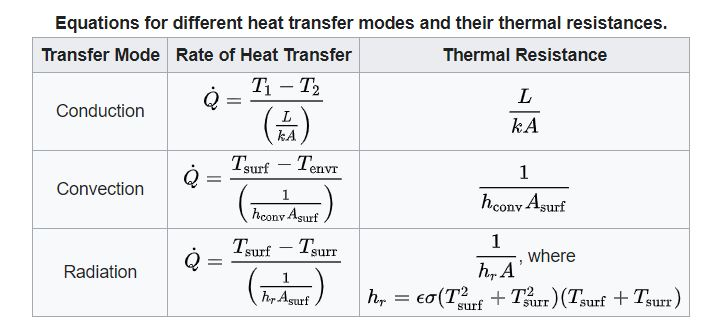
\includegraphics[width=0.8\columnwidth]{Pictures/heat transfer mode.JPG}
	\caption[Short title]{Heat transfer modes\cite{GIGO}}
	\label{table_1}
\end{figure}
\newpage

In \cite{HTTHERMO} and \cite{FUND} the expressions in Fig.\ref{table_1} are derived.
For conduction, the expression for absolute thermal resistance is:  

\begin{equation}
	R = \frac{L}{kA} \qquad \left[ \frac{K}{W} \right]
\end{equation}

\begin{itemize}
    \item $L$ is the distance over which heat transfer takes place, or the thickness of the material $[m]$.
    \item $k$ (also denoted with $\lambda$) is the thermal conductivity of the material. [$\frac{W}{mK}$]. 
    \item $A$ is the conductive surface area  $[m^2]$.
    \item Thermal resistivity is the reciprocal of thermal conductivity and can be expressed as $r =\frac{1}{k}$  in $[\frac{mK}{W}]$

\end{itemize}


For convection and radiation the expression for thermal resistance is: $R = \frac{1}{h \cdot A}$ [$\frac{K}{W}$].

\begin{itemize}
    \item $A$ is the surface area where the heat transfer takes place $[m^2]$.
    \item $h$ is the heat transfer coefficient  [$\frac{W}{m^2K}$]
\end{itemize}


The $R$-value (in Dutch: $R$-waarde or $R_d$-waarde) of a building material \cite{Rvalues_insulation} is the thermal resistance of a square meter surface.
It can be calculated by multiplying the thermal \emph{resistivity} with the thickness of the material in  $m$.
Alternatively it is calculated by dividing the material thickness by the thermal \emph{conductivity} $k$ or $\lambda$.

\begin{equation}
	\text{R-value} = r \cdot L  \qquad \text{or} \qquad  \text{R-value} = \frac{L}{k}  \qquad \text{or} \qquad  
	\text{R-value} = \frac{L}{\lambda}  \qquad \left[m \cdot \frac{m \cdot K}{W} \right] = \left[\frac{m^2 \cdot K}{W}\right] 
\end{equation}


Some typical heat transfer $R$-values are: \cite{OVERALL}: 

\begin{itemize}
	\item Static layer of air, 40 mm thickness (1.57 in)  : R = 0.18 [$\frac{m^2K}{W}$].
	\item Inside heat transfer resistance, horizontal current : R = 0.13 [$\frac{m^2K}{W}$]. 
	\item Outside heat transfer resistance, horizontal current : R = 0.04 [$\frac{m^2K}{W}$].
	\item Inside heat transfer resistance, heat current from down upwards : R = 0.10 [$\frac{m^2K}{W}$].
	\item Outside heat transfer resistance, heat current from above downwards : R = 0.17 [$\frac{m^2K}{W}$].
\end{itemize}


\textbf{Note}: in Dutch building physics, $R$-values with subscripts are used:
\begin{itemize}
	\item $R_d$-waarde is used for the $R$-value of a homogeneous building material. $ R = \frac{L}{\lambda} $
	\item $R_c$-waarde (compound, construction) is used for the $R$-value of a surface consisting of several building materials. $R_c$-waarden are calculated as the surface-area weighted sum of $R_d$-waarden of the building materials. 
	For the simplest roof surface, $R_c$ is a linear combination of the $R$-values of the wooden joists and girders (spanten en gordingen) and the areas in between with a certain insulation material sandwich.
	The $R$-value of the insulation sandwich, in its turn, is the sum of the $R$-values of the materials in the sandwich. From inside out, this sandwich may consist of \textit{e.g.} a 9.5 mm plaster board, a PIR/PUR insulation panel, an air gap and a wooden roof deck. All types of $R$-value have the dimension $ [\frac{m^2 \cdot K}{W}] $.
\end{itemize}

\begin{figure}[H]
	\centering
	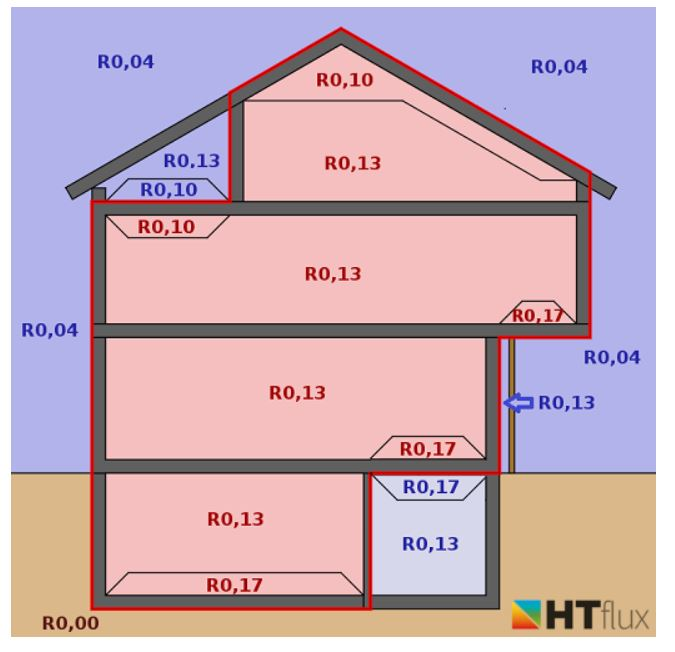
\includegraphics[width=0.8\columnwidth]{Pictures/Overview of heat resistances.JPG}
	\caption[Short title]{An overview of $R$-values for heat transfer \cite{SURFREST}.}
	\label{fig:overview}
\end{figure}


The standard R\textsubscript{c}-values that have been used for facades, roof and floor until 2020 are summarized in Fig.\ref{fig:Rcvalues}:

\begin{figure}[H]
	\centering
	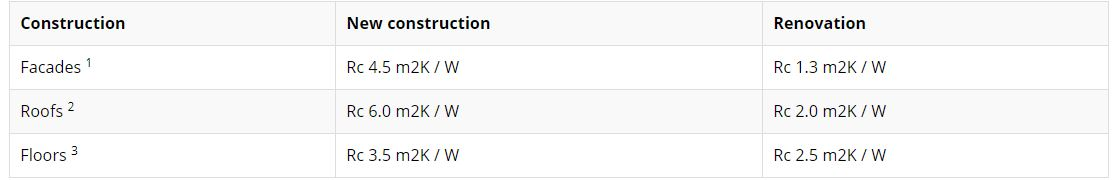
\includegraphics[width=1.0\columnwidth]{Pictures/Rc_values_2020.JPG}
	\caption[Short title]{R\textsubscript{c} Values \cite{ISOL}}
	\label{fig:Rcvalues}
\end{figure}

New standard values will be used from 1-1-2021, since the building standard NEN 1068 will be replaced by the NTA 8800 standard. The old and new situation is described in "EnergieVademecum Energiebewust ontwerpen van nieuwbouwwoningen", Hoofdstuk 5: Thermische isolatie, thermische bruggen en luchtdichtheid.
\cite{ISSO}.

\begin{figure}[H]
	\centering
	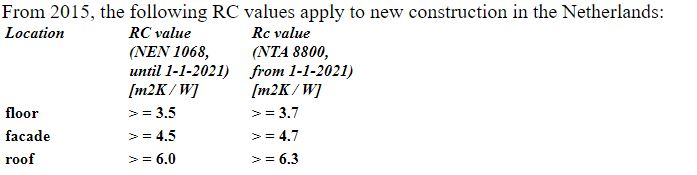
\includegraphics[width=1.0\columnwidth]{Pictures/Rc_values_2021.JPG}
	\caption[Short title]{R\textsubscript{c} Values \cite{RVALUE}}
	\label{fig:newRc}
\end{figure}

The values used for different types of houses such as: row houses, detached houses and apartments can be found in the document "Voorbeeldwoningen 2011" \cite{VOORBEELD}. An example with values for a common type of row house, built in the period from 1975 to 1991 is shown in Fig. \ref{row_house}:


\begin{figure}[H]
	\centering
	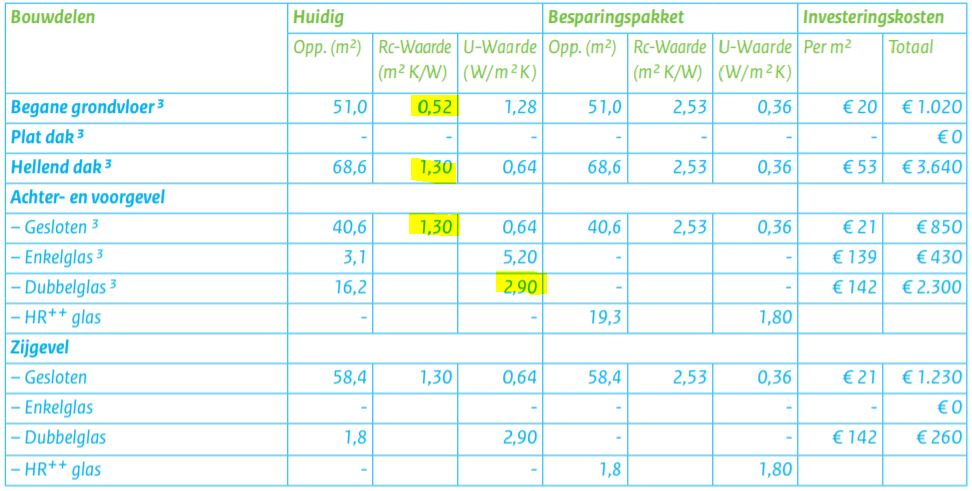
\includegraphics[width=0.8\columnwidth]{Pictures/row_house_1975-1991.JPG}
	\caption[Short title]{R\textsubscript{c}-values for a row house type built between 1975-1991 \cite{VOORBEELD}}
	\label{row_house}
\end{figure} 
\newpage

\subsection{Dwelling (envelope) model analogous to a 2R-2C network}

The heat flow will be modelled by analogy to an electrical circuit where heat transfer rate is analogous to by current, temperature difference is analogous to potential difference, heat sources are represented by constant current sources, absolute thermal resistances are represented by resistors and \textbf{thermal capacitance} heat capacity ? by capacitors \cite{AbsTR}. Figure \ref{fig:Analogies} summarizes the similar term use in different fields.

\begin{figure}[H]
	\centering
	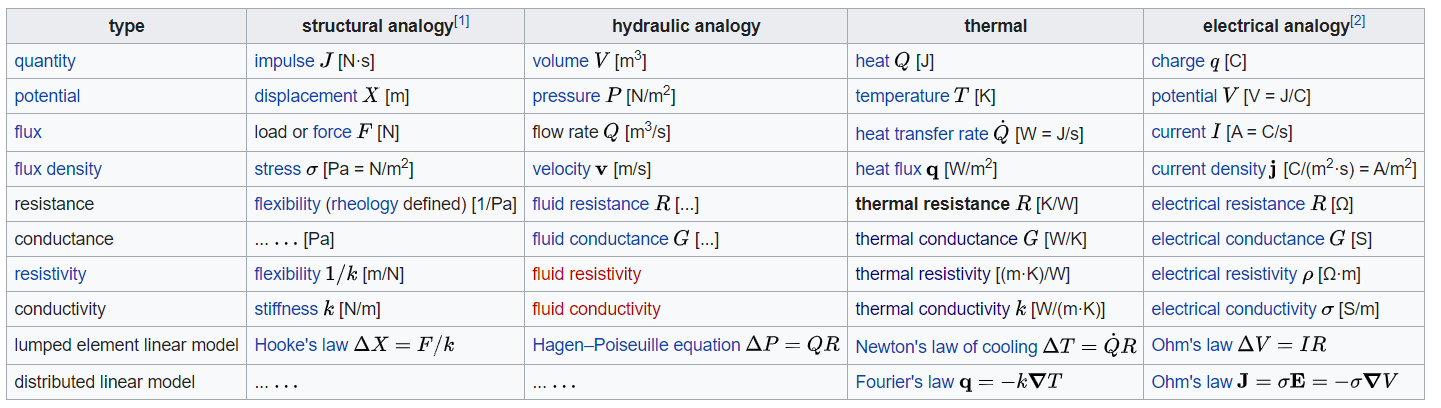
\includegraphics[width=1.0\columnwidth]{Pictures/Analogies.png}
	\caption[Short title]{Table of Analogies  \cite{AbsTR}}
	\label{fig:Analogies}
	\end{figure} 

The 2R-2C house model structure is implemented as described below. The schematic of an envelope house model has been shown in figure  \ref{fig:envelope2R2C} and the equivalent electrical 2R-2C network with components and topology is given in fig  \ref{fig:elec2R2C}.

\begin{figure}[H]
	\centering
	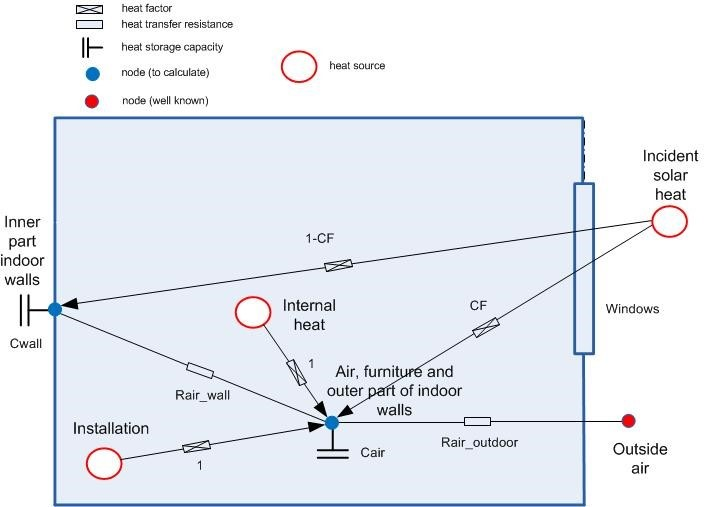
\includegraphics[width=1.0\columnwidth]{Pictures/envelopRC.jpg}
	\caption[Short title]{Schematic of envelope model}
	\label{fig:envelope2R2C}
	\end{figure} 
	

\begin{figure}[H]
	\centering
	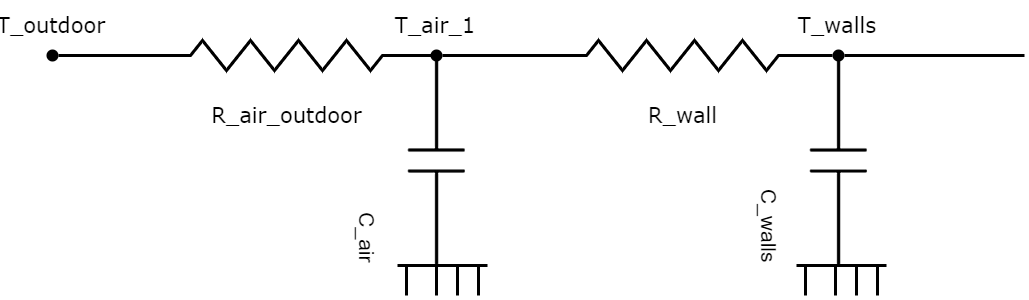
\includegraphics[width=1.0\columnwidth]{Pictures/2R2C_Model.png}
	\caption[Short title]{2R-2C house model}
	\label{fig:elec2R2C}
	\end{figure}
	
The model consists of two heat capacities C\textsubscript{air, indoor} and C\textsubscript{wall} and two resistances R\textsubscript{wall} and R\textsubscript{air, outdoor}. The incident solar energy is divided between C\textsubscript{wall} and C\textsubscript{air} through the convection factor CF. It is assumed that both internal heat (lighting, occupancy and electric devices) and supplied heat (installation) initially heat up the indoor air. In Fig. \ref{fig:envelope2R2C}, they are fully released at the T\textsubscript{air} node. 

 It is also assumed that furniture and the \textbf{surface part} of the walls have the same temperature as the air \textbf{and the wall mass is divided between the air and wall mass}. Thus, the heat capacity of the air node consists of the air heat capacity, furniture heat capacity and the heat capacity \textbf{of a part of the walls}. \textbf{Appendix A} presents the coefficients in the dwelling model. In the resistance R\textsubscript{air, outdoor} the influence of heat transmission through the outdoor walls and natural ventilation is considered. 
 
For the air and wall nodes the following power balances can be set up: 

\begin{equation}
C_{air}\frac{dT_{air}}{dt}=\frac{T_{outdoor}-T_{air}}{R_{air_{\_}outdoor}} + \frac{T_{wall}-T_{air}}{R_{air_{\_}wall}} + \dot{Q}_{inst} + \dot{Q}_{internal} + CF\cdot\dot{Q}_{solar}
\end{equation}

\begin{equation}
C_{wall}\frac{dT_{wall}}{dt}=\frac{T_{air}-T_{wall}}{R_{air_{\_}wall}} + (1-CF)\cdot\dot{Q}_{solar}
\end{equation}


 \begin{itemize}
      \item $CF$: convection factor (solar radiation): the convection factor is the part of the solar radiation that enters the room and is released directly convectively into the room.
      \item $\dot{Q}_{inst}$: delivered heat from heating system (radiator) [W].
      \item $\dot{Q}_{inernal}$: internal heat [W].
      \item $\dot{Q}_{solar}$: heat from solar irradiation [W].
      \item $T_{air}$: indoor air temperature $^o$C.
      \item $T_{outdoor}$: outdoor temperature $^o$C.
      \item $T_{wall}$: wall temperature $^o$C.
      \item $R_{air_{\_}wall}$: walls surface resistance [$\frac{K}{W}$].
      \item $R_{air_{\_}outdoor}$: outdoor surface resistance [$\frac{K}{W}$].
      \item $C_{air}$: air thermal capacitance (heat capacity) [$\frac{J}{K}$]\cite{Thermalmass}.
      \item $C_{wall}$: wall thermal capacitance (heat capacity) [$\frac{J}{K}$]\cite{Thermalmass}.
    \end{itemize}

\newpage   

Total heat transfer of solar irradiation through the glass windows. 
\begin{equation}
\dot{Q}_{solar}=g.\sum(A_{glass}.\dot{q}_{solar})
\end{equation}

\begin{itemize}
    \item $\dot{q}_{solar}$: solar radiation on the outdoor walls [$\frac{W}{m^2}$]. 
    \item g: g value of the glass (ZTA in dutch) [0..1]\cite{zontoetreding}
    \item A: glass surface [$m^2$].
\end{itemize}

%7.6.6.1.2 Ramen met niet-verstrooiende beglazing NTA8800
%https://help.dgmr.nl/bink9/zontoetredingsfactor-zta.html
%https://www.joostdevree.nl/shtmls/zta.shtml
%ISSO-Handboek Zonnestraling: 5.5.1 en 5.2


\newpage

\section{Lumped-element thermal model of a building}

Heat generation and transport inside a building, with heat loss to the surrounding outdoor environment is governed by the same laws of conduction, convection and radiation as elsewhere. A number of approximations is made, however, which will be treated below:

\subsection{Heat Conduction: Fourier's Law}

Heat transport \emph{within} a solid material is governed by conduction, according to Fourier's Law, illustrated in Figure \ref{fig:heatcond_1d}.
One side of a rectangular solid is held at temperature $T_1$, while the opposite side is held at a lower temperature, $T_2$. The other four sides are insulated so that heat can flow only in the $x$-direction. For a given material, it is found that the rate, $\dot{Q_x}$ , at which heat (thermal
energy) is transferred from the hot side to the cold side (the \emph{heat transfer rate}) is proportional to the cross-sectional area, $A$, across which the heat flows; the temperature difference, $T_1 - T_2$; and inversely proportional to
the thickness, $\Delta x$, of the material. That is:

\begin{equation}
	\label{eq:fourierlaw}
	\dot{Q_x} = - kA \frac{\Delta T}{\Delta x}
\end{equation}

\begin{figure}[H]
	\centering
	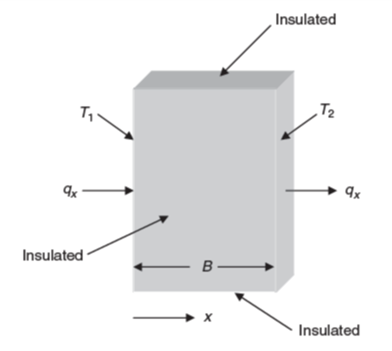
\includegraphics[width=0.5\columnwidth]{Pictures/heat_conduction_1d.png}
	\caption[Short title]{One-dimensional heat conduction in a solid}
	\label{fig:heatcond_1d}
\end{figure} 

The constant of proportionality, $k$, is called the \emph{thermal conductivity}. Equation \eqref{eq:fourierlaw} is also applicable to heat conduction in liquids and gases. However, when temperature differences exist in fluids, convection currents tend to be set up, so that heat is generally not transferred solely by the mechanism of conduction. The thermal conductivity is a property of the material. Values may be found in various handbooks and compendiums of physical property data.

The form of Fourier’s law given by Equation \eqref{eq:fourierlaw} is valid only when the thermal conductivity can be assumed constant. A more general result can be obtained by writing the equation for an element of differential thickness. in the limit as $\Delta x$ approaches zero, $\frac{\Delta T}{\Delta x} \rightarrow \frac{d T}{d x}$. Thus, substituting in Equation \eqref{eq:fourierlaw} gives:

\begin{equation}
	\label{eq:fourierdiff}
	\dot{Q_x} = - kA \frac{d T}{d x}
\end{equation}

Equation \eqref{eq:fourierdiff} is not subject to the restriction of constant $k$. Furthermore, when $k$ is constant, it can be integrated to yield Equation \eqref{eq:fourierlaw}. Hence, Equation \eqref{eq:fourierdiff} is the general one-dimensional form of Fourier’s law. The negative sign is necessary because heat flows in the positive $x$-direction when the temperature decreases in the $x$-direction. Thus, according to the standard sign convention that
$\dot Q_x$ is positive when the heat flow is in the positive $x$-direction, $\dot Q_x$ must be positive when $dT/dx$ is negative. 

\subsubsection{More than one dimension}

It is often convenient to formulate Fourier's Law in the original phrasing: the \emph{heat flux} $ \dot{\varphi}$  is proportional to the \emph{temperature gradient}. We divide \eqref{eq:fourierdiff} by the area to give:

\begin{equation}
	\label{eq:fourierflux}
	\dot{\varphi_x} \equiv \frac{\dot Q_x}{A}- k \frac{d T}{d x}
\end{equation}

where $\dot{\varphi_x}$ is the heat flux. It has units of $\frac{J}{s \cdot m^2} = \frac{W}{m^2}$. 
Thus, the units of $k$ are $\frac{W}{m \cdot K}$.

Equation \eqref{eq:fourierflux} is restricted to the situation in which heat flows in the $x$-direction
only. In the general case in which heat flows in all three coordinate directions, the total heat flux is obtained by vector addition of adding the fluxes in the coordinate directions. Thus,

\begin{equation}
	\label{eq:flux3d}
	\boldsymbol{\dot{\varphi}} = \dot{\varphi_x} \mathbf{i} + \dot{\varphi_y} \mathbf{j} + \dot{\varphi_z} \mathbf{k}
\end{equation}

where $\boldsymbol{\dot{\varphi}}$ is the heat flux vector and \textbf{i}, \textbf{j}, \textbf{k} are unit vectors in the x-, y-, z-directions, respectively.

Each of the component fluxes is given by a one-dimensional Fourier expression as follows:

\begin{equation}
	\begin{aligned}
		\label{eq:fourier3d}
		\dot{\varphi_x} = - k \frac{\partial T}{\partial x} & \qquad & \dot{\varphi_y} = - k \frac{\partial T}{\partial y} & \qquad & \dot{\varphi_z} = - k \frac{\partial T}{\partial z}
	\end{aligned}
\end{equation}

Partial derivatives are used here since the temperature now varies in all three directions. Substituting
the above expressions for the fluxes into Equation \eqref{eq:flux3d} gives:

\begin{equation}
	\label{eq:fouriercart}
	\boldsymbol{\dot{\varphi}} = -k \left(\frac{\partial T}{\partial x} \mathbf{i} + \frac{\partial T}{\partial y} \mathbf{j} + \frac{\partial T}{\partial z} \mathbf{k} \right)
\end{equation}

The vector in parenthesis is the temperature gradient vector, and is denoted by $\nabla T$. Hence,

\begin{equation}
	\label{eq:fouriernabla}
	\boldsymbol{\dot{\varphi}} = -k \nabla T
\end{equation}

Equation \eqref{eq:fouriernabla} is the three-dimensional form of Fourier’s law. It is valid for homogeneous, isotropic materials for which the thermal conductivity is the same in all directions. Fourier’s law states that heat flows in the direction of greatest temperature decrease.

\subsubsection{The Heat Conduction Equation}

The solution of problems involving heat conduction in solids can, in principle, be reduced to the
solution of a single differential equation, the \emph{heat conduction equation}. The equation can be derived
by making a thermal power balance on a differential volume element in the solid. For the case of
conduction in the $x$-direction only, such a volume element is illustrated in Figure \ref{fig:element_1d}. 

\begin{figure}[H]
	\centering
	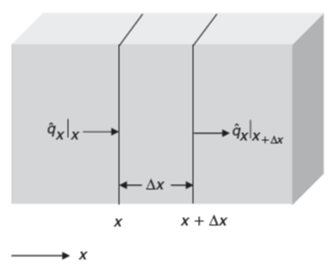
\includegraphics[width=0.5\columnwidth]{Pictures/Element.png}
	\caption[Short title]{Differential element for 1D heat conduction}
	\label{fig:element_1d}
\end{figure}

The rate at which thermal energy enters the volume element across the face at $x$ is given by the
product of the heat flux and the cross-sectional area, $\dot{\varphi_x}|_x \cdot A$.
Similarly, the rate at which thermal energy leaves the element across the face at $x + \Delta x$ is $\dot{\varphi_x}|_{x + \Delta x} \cdot A$. 

A heat generation term appears in the equation because the balance is made on thermal energy, not
total energy. For example, thermal energy may be generated within a solid by an electric current
or by decay of a radioactive material.

For a homogeneous heat source of strength $\dot{q}$ \emph{per unit volume}, the net rate of generation is $\dot{q}A \Delta x$. Finally, the rate of accumulation of heat in the material is given by the time derivative of the thermal energy content of the volume element, which is $\rho c(T - T_{ref} )A\Delta x$, where $T_{ref}$ is an arbitrary reference temperature. Thus, the balance equation
becomes:

\begin{equation}
	\label{eq;heatbalance}
	\left( \dot{\varphi_x}|_x - \dot{\varphi_x}|_{x + \Delta x} \right)A + \dot{q}A \Delta x = \rho c  \frac{\partial T}{\partial t}A\Delta x
\end{equation}

It has been assumed here that the density, $\rho$, and heat capacity, $c$, are constant. 

Dividing by $A \Delta x$ and taking the limit as $\Delta x \rightarrow 0 $ yields:

\begin{equation}
	\rho c  \frac{\partial T}{\partial t} = -\frac{\partial \dot{\varphi_x}}{\partial x} + \dot{q}
\end{equation}

Using Fourier’s law as given by Equation \eqref{eq:fourierflux}, the balance equation becomes:

\begin{equation}
	\rho c  \frac{\partial T}{\partial t} = \frac{\partial}{\partial x} \left(\frac{k \partial T}{\partial x} \right)+ \dot{q}
\end{equation}

When conduction occurs in all three coordinate directions, the balance equation contains y- and
z-derivatives analogous to the x-derivative. The balance equation then becomes:

\begin{equation}
	\label{eq:heat3d}
	\rho c  \frac{\partial T}{\partial x} = \frac{\partial}{\partial x} \left(\frac{k \partial T}{\partial x} \right)  + \frac{\partial}{\partial y} \left(\frac{k \partial T}{\partial y} \right) + \frac{\partial}{\partial z} \left(\frac{k \partial T}{\partial z} \right) + \dot{q}
\end{equation}

When $k$ is constant, it can be taken outside the derivatives and Equation \eqref{eq:heat3d} can be written as:	

\begin{equation}
	\frac{\rho c}{k}  \frac{\partial T}{\partial t} = \frac{\partial^2 T}{\partial x^2}  + \frac{\partial^2 T}{\partial y^2} + \frac{\partial^2 T}{\partial z^2} + \frac{\dot{q}}{k}
\end{equation}

or

\begin{equation}
	\frac{1}{\alpha} \frac{\partial T}{\partial t} = \nabla^2 T + \frac{\dot{q}}{k}
\end{equation}

where $\alpha \equiv k /\rho c$ is the \emph{thermal diffusivity} and $\nabla^2$ is the Laplacian operator. The thermal diffusivity has units of $m^2/s$.


\subsection{Convection: Newton's Law of cooling}

When a solid is \emph{immersed} in a fluid or atmospheric gas, heat transfer on the interface occurs by convection. This phenomenon is governed by Newton's Law of cooling:

“The rate of heat lost by a body is directly proportional to the temperature difference of a body and its surroundings”

\begin{equation}
	\label{eq:newtonlaw}
	\dot{Q_x} = - hA \Delta T
\end{equation}

\subsection{Radiation}

\subsection{Approximations: A Simplified Model}

In building physics, it is often assumed that Fourier's Law is valid in the form of Eq. \eqref{eq:fourierlaw}. This can be done under the condition that 

\begin{equation}
	\begin{aligned}
	    \nabla^2 T \equiv 0 & \rightarrow & \frac{\partial T}{\partial \mathbf{r}} = constant
    \end{aligned}
\end{equation}

\subsection{Lumped-element matrix representation}

We take the 2R-2C lumped-element model from Section 2:

\begin{figure}[H]
	\centering
	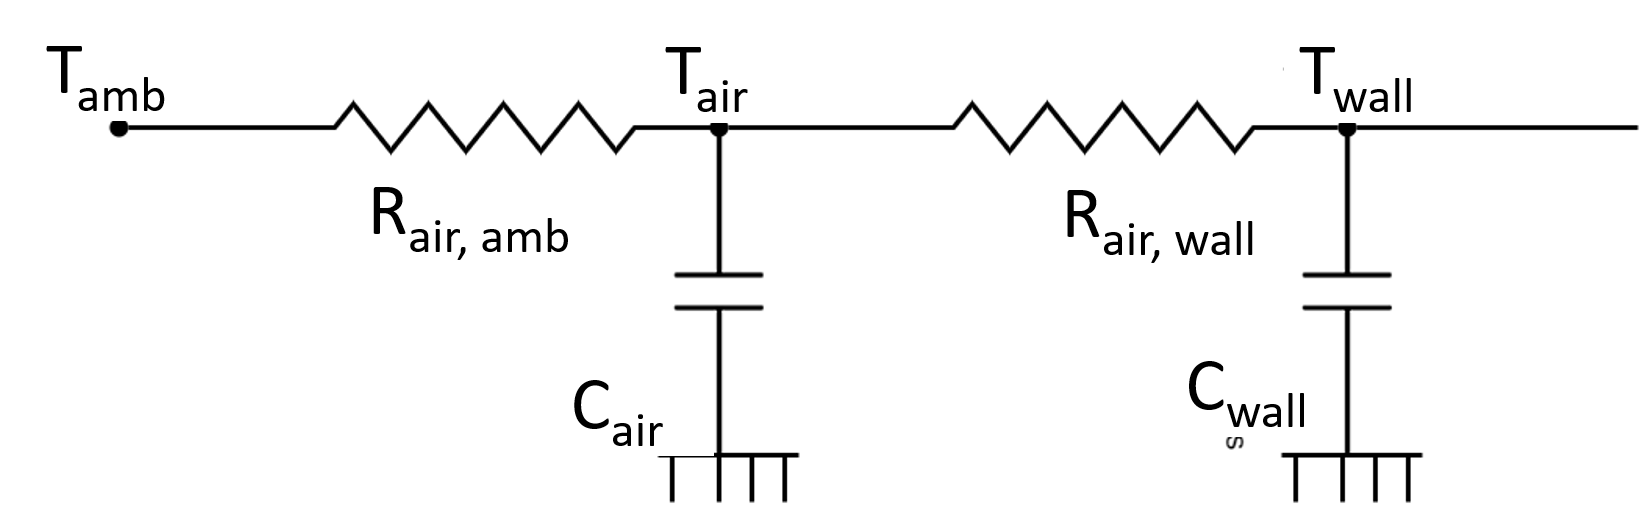
\includegraphics[width=0.7\columnwidth]{Pictures/2R2Cmodel_rev.png}
	\caption[Short title]{2R-2C house model revisited}
	\label{fig:elec2R2Cbis}
\end{figure}

The differential equations are:

\begin{equation}
	\begin{aligned}
	C_{air}\frac{dT_{air}}{dt} &=\frac{T_{amb}-T_{air}}{R_{air, amb}} + \frac{T_{wall}-T_{air}}{R_{air, wall}} + \dot{Q}_{heat, air} + \dot{Q}_{int, air} + \dot{Q}_{solar, air} 
	\\ \\
	C_{wall}\frac{dT_{wall}}{dt} &=\frac{T_{air}-T_{wall}}{R_{air, wall}} + \dot{Q}_{solar, wall}
    \end{aligned}
\end{equation}

Writing out the differential equations in the classical notation:

\begin{equation}
	\begin{aligned}
		C_{air}\frac{dT_{air}}{dt} &= \left[ \frac{-1}{R_{air, amb}} + \frac{-1}{R_{air, wall}} \right]  \cdot T_{air}  + \frac{1}{R_{air, wall}} \cdot T_{wall} + \frac{1}{R_{air, amb}} \cdot T_{amb} + \dot{Q}_{heat, air} + \dot{Q}_{int, air} + \dot{Q}_{solar, air} 
		\\ \\
		C_{wall}\frac{dT_{wall}}{dt} &= \frac{1}{R_{air, wall}} \cdot T_{air} + \frac{-1}{R_{air, wall}}   \cdot T_{wall} + \dot{Q}_{solar, wall}
	\end{aligned}
\end{equation}

The differential equations can be written in matrix notation as:

\begin{subequations}
	\label{eq:matnot}
	\begin{align}
	\mathbf{C} \cdot \boldsymbol{\dot{\theta}} = - \mathbf{K} \cdot \boldsymbol{\theta} + \mathbf{\dot{q}} \\ 
	\mathbf{C} \cdot \boldsymbol{\dot{\theta}} + \mathbf{K} \cdot \boldsymbol{\theta} = \mathbf{\dot{q}}
	\end{align}
\end{subequations}

with:

\begin{equation}
	\mathbf{C} \cdot \boldsymbol{\dot{\theta}} =
	\begin{bmatrix}
		C_{air} & 0 \\
		0 &  C_{wall}
	\end{bmatrix}
    \cdot
    \begin{bmatrix}
    	\frac{dT_{air}}{dt} \\
    	\frac{dT_{wall}}{dt}
    \end{bmatrix}
\end{equation}

\begin{equation}
	\mathbf{K} \cdot \boldsymbol{\theta} =
	\begin{bmatrix}
		\frac{1}{R_{air, amb}} + \frac{1}{R_{air, wall}} & \frac{-1}{R_{air, wall}} \\
		\frac{-1}{R_{air, wall}} &  \frac{1}{R_{air, wall}}
	\end{bmatrix}
	\cdot
	\begin{bmatrix}
		T_{air} \\
		T_{wall}
	\end{bmatrix}
\end{equation}

\begin{equation}
	\mathbf{\dot{q}} =
	\begin{bmatrix}
		\frac{1}{R_{air, amb}} \cdot T_{amb} + \dot{Q}_{heat, air} + \dot{Q}_{int, air} + \dot{Q}_{solar, air} \\
		\dot{Q}_{solar, wall}
	\end{bmatrix}
\end{equation}

Written out, the differential equation according to \eqref{eq:matnot} becomes:

\begin{equation}
	\begin{aligned}
		\begin{bmatrix}
			C_{air} & 0 \\
			0 &  C_{wall}
		\end{bmatrix}
		\cdot
		\begin{bmatrix}
			\frac{dT_{air}}{dt} \\
			\frac{dT_{wall}}{dt}
		\end{bmatrix}
		=
		\begin{bmatrix}
			\frac{-1}{R_{air, amb}} + \frac{-1}{R_{air, wall}} & \frac{1}{R_{air, wall}} \\
			\frac{1}{R_{air, wall}} &  \frac{-1}{R_{air, wall}}
		\end{bmatrix}
		\cdot
		\begin{bmatrix}
			T_{air} \\
			T_{wall}
		\end{bmatrix}
		+ \\ \\
		\begin{bmatrix}
			\frac{1}{R_{air, amb}} \cdot T_{amb} + \dot{Q}_{heat, air} + \dot{Q}_{int, air} + \dot{Q}_{solar, air} \\
			\dot{Q}_{solar, wall}
		\end{bmatrix}
	\end{aligned}
\end{equation}

In the alternative notation:

\begin{equation}
	\begin{aligned}
	\begin{bmatrix}
	    C_{air} & 0 \\
	    0 &  C_{wall}
    \end{bmatrix}
    \cdot
    \begin{bmatrix}
    	\frac{dT_{air}}{dt} \\
    	\frac{dT_{wall}}{dt}
    \end{bmatrix}
    +
    	\begin{bmatrix}
    	\frac{1}{R_{air, amb}} + \frac{1}{R_{air, wall}} & \frac{-1}{R_{air, wall}} \\
    	\frac{-1}{R_{air, wall}} &  \frac{1}{R_{air, wall}}
    \end{bmatrix}
    \cdot
    \begin{bmatrix}
    	T_{air} \\
    	T_{wall}
    \end{bmatrix}
    = \\ \\
    \begin{bmatrix}
        \frac{1}{R_{air, amb}} \cdot T_{amb} + \dot{Q}_{heat, air} + \dot{Q}_{int, air} + \dot{Q}_{solar, air} \\
    	\dot{Q}_{solar, wall}
    \end{bmatrix}
	\end{aligned}
\end{equation}

The lumped-element equations above are systems of \emph{first-order ordinary differential equations} (ODE). The first order derivative is with respect to \emph{time}. The (silent) assumption that heat conduction within the air and the wall of the previous 2R-2C model is \emph{faster} than the exchange of heat at the \emph{interfaces} between air and wall and air and ambient surroundings has replaced all spatial information from the \emph{second-order partial differential equations} (PDE) that govern conductive heat transport \emph{within} materials.

Therefore, the lumped-element equations can be solved by:
\begin{itemize}
	\item the \textsf{odexxx} in Matlab., preferrably \textsf{ode45}.
	\item the \textsf{state-space} module in Simulink, after conversion to a state-space representation.
	\item the \textsf{scipy.integrate.solve\_ivp} function in Python. In older code, \textsf{scipy.integrate.odeint} is still encountered.
	\item in C++ several options exist, similar to the options in Python.
\end{itemize}

The routines in Matlab, Simulink and Python need a \emph{model function} that provides the vector $\boldsymbol{\dot{\theta}}$ for evaluation at any time instance chosen by the algorithm. The equations \eqref{eq:matnot} then should be cast in the following form by left multiplication with $\mathbf{C^{-1}}$.

\begin{subequations}
	\label{eq:matnot_ivp}
	\begin{align}
		\mathbf{C}^{-1} \cdot \mathbf{C} \cdot \boldsymbol{\dot{\theta}} = - \mathbf{C}^{-1} \cdot \mathbf{K} \cdot \boldsymbol{\theta} + \mathbf{C}^{-1} \cdot \mathbf{\dot{q}} \\ 
        \boldsymbol{\dot{\theta}} = - \mathbf{C}^{-1} \cdot \mathbf{K} \cdot \boldsymbol{\theta} + \mathbf{C}^{-1} \cdot \mathbf{\dot{q}}
	\end{align}
\end{subequations}

Since $\mathbf{C}$ is a \emph{diagonal} matrix with positive elements only, its inverse exists and contains the reciprocal elements on its diagonal:

\begin{equation}
	\mathbf{C^{-1}} =
	\begin{bmatrix}
		\frac{1}{C_{air}} & 0 \\
		0 &  \frac{1}{C_{wall}}
	\end{bmatrix}
\end{equation}

This provides the division by the lumped thermal capacitances of the air and wall compartments in the model, necessary for the calculating the derivative vector $\boldsymbol{\dot{\theta}}$ in the model functions. 

\subsection{Extension of the method to larger lumped-element networks}

Take a house model with two stories. Each level in the building is described with a 2R-2C model. Heat transfer occurs between the ground floor and the 1st floor.

\begin{figure}[H]
	\centering
	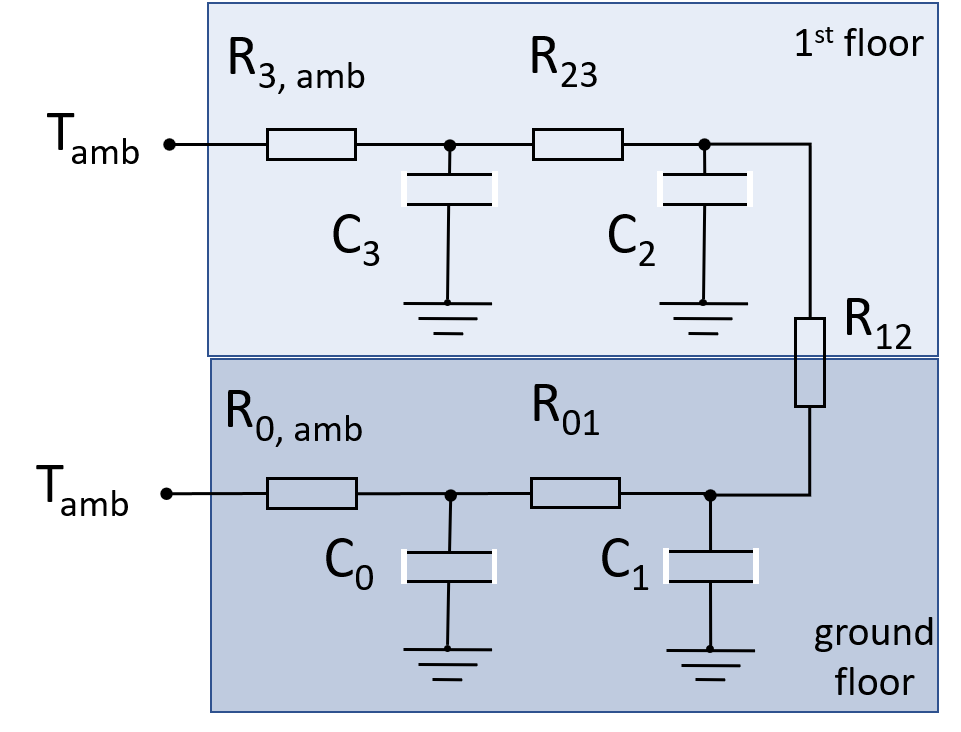
\includegraphics[width=0.6\columnwidth]{Pictures/5R4C.png}
	\caption[Short title]{5R-4C house model}
	\label{fig:elec4R5C}
\end{figure}

\begin{equation}
	\mathbf{C} \cdot \boldsymbol{\dot{\theta}} =
	\begin{bmatrix}
		C_{0} & 0 & 0 & 0\\
		0 &  C_{1} & 0 & 0 \\
		0 & 0 & C_{2} & 0\\
		0 & 0 & 0 & C_{3}
	\end{bmatrix}
	\cdot
	\begin{bmatrix}
		\frac{dT_{0}}{dt} \\
		\frac{dT_{1}}{dt} \\
	    \frac{dT_{2}}{dt} \\
	    \frac{dT_{3}}{dt} 
	\end{bmatrix}
\end{equation}

\begin{equation}
	\mathbf{K} \cdot \boldsymbol{\theta} =
	\begin{bmatrix}
		\frac{1}{R_{0, amb}} + \frac{1}{R_{01}} & \frac{-1}{R_{01}} & 0 & 0 \\
		\frac{-1}{R_{01}} &  \frac{1}{R_{01}} + \frac{1}{R_{12}} & \frac{-1}{R_{12}} & 0 \\
		 0 & \frac{-1}{R_{12}} & \frac{1}{R_{12}} + \frac{1}{R_{23}}  & \frac{-1}{R_{23}}\\
	 	 0 & 0 & \frac{-1}{R_{23}} &  \frac{1}{R_{3, amb}} + \frac{1}{R_{23}} \\
	\end{bmatrix}
	\cdot
	\begin{bmatrix}
		T_{0} \\
		T_{1} \\
		T_{2} \\
		T_{3}
	\end{bmatrix}
\end{equation}

\begin{equation}
	\mathbf{\dot{q}} =
	\begin{bmatrix}
		\frac{1}{R_{0, amb}} \cdot T_{amb} + \dot{Q}_{heat, 0} + \dot{Q}_{int, 0} + \dot{Q}_{solar, 0} \\
		\dot{Q}_{solar, 1} \\
		\dot{Q}_{solar, 2} \\
		\frac{1}{R_{3, amb}} \cdot T_{amb} + \dot{Q}_{heat, 3} + \dot{Q}_{int, 3} + \dot{Q}_{solar, 3}
	\end{bmatrix}
\end{equation}

\subsection{Alternative representation of 5R-4C model}

The 5R4C model of the previous section can be built from two 2R2C models, one for the ground floor and one for the first floor. The thermal resistance between the construction nodes of the ground and first floor is then added, $R_{13}$ in the figure:
 
\begin{figure}[H]
	\centering
	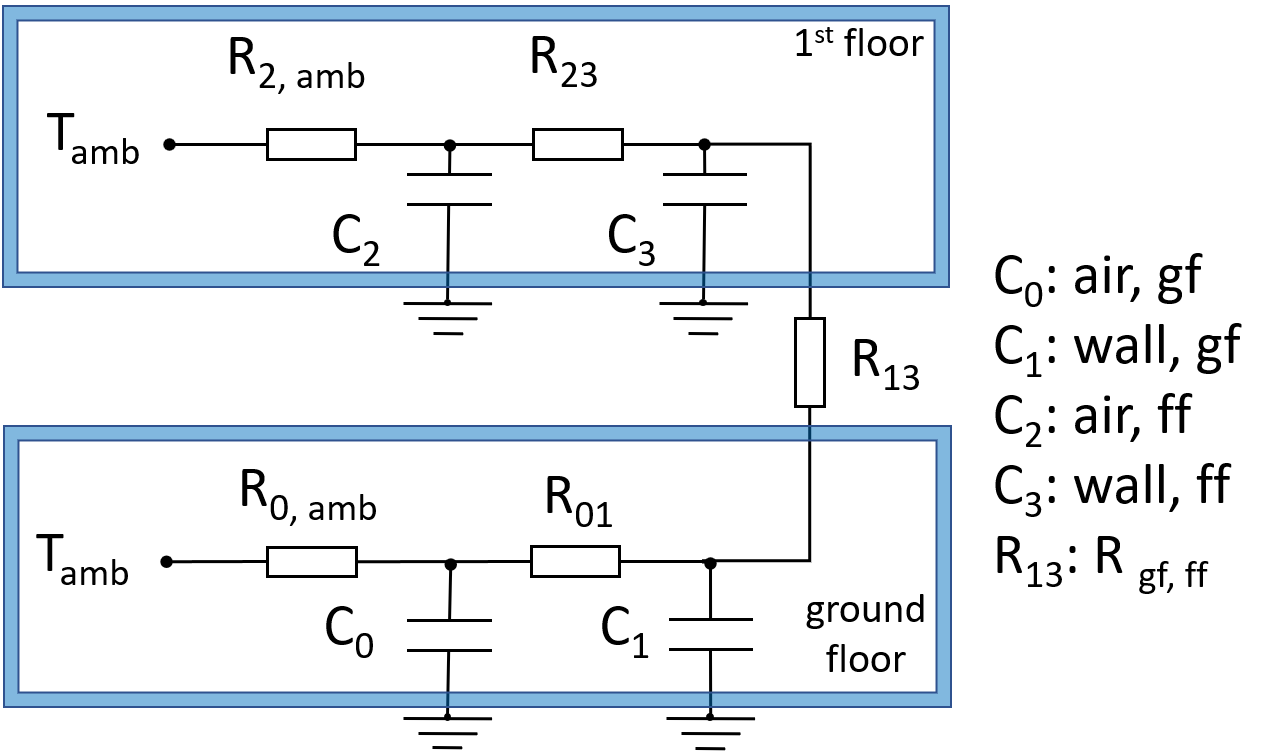
\includegraphics[width=0.6\columnwidth]{Pictures/5R4C_alternative.png}
	\caption[Short title]{5R-4C house model, alternative representation}
	\label{fig:alt5R4C}
\end{figure}

As can be seen in the matrices below, adding $R_{13}$ to the ground floor and first floor "chains" results in a non-symmetric matrix. It has to determined if this disadvantage outweighs the benefit of adding "chains".

\begin{equation}
	\mathbf{C} \cdot \boldsymbol{\dot{\theta}} =
	\begin{bmatrix}
		C_{0} & 0 & 0 & 0\\
		0 &  C_{1} & 0 & 0 \\
		0 & 0 & C_{2} & 0\\
		0 & 0 & 0 & C_{3}
	\end{bmatrix}
	\cdot
	\begin{bmatrix}
		\frac{dT_{0}}{dt} \\
		\frac{dT_{1}}{dt} \\
		\frac{dT_{2}}{dt} \\
		\frac{dT_{3}}{dt} 
	\end{bmatrix}
\end{equation}

\begin{equation}
	\mathbf{K} \cdot \boldsymbol{\theta} =
	\begin{bmatrix}
		\frac{1}{R_{0, amb}} + \frac{1}{R_{01}} & \frac{-1}{R_{01}} & 0 & 0 \\
		\frac{-1}{R_{01}} &  \frac{1}{R_{01}} + \color{red} \frac{1}{R_{13}} & 0 & \color{red} \frac{-1}{R_{13}} \\
		0 & 0 & \frac{1}{R_{2, amb}} + \frac{1}{R_{23}} & \frac{-1}{R_{23}} \\
		0 & \color{red}\frac{-1}{R_{13}} & \frac{-1}{R_{23}}  & \frac{1}{R_{23}} + \color{red}\frac{1}{R_{13}}
	\end{bmatrix}
	\cdot
	\begin{bmatrix}
		T_{0} \\
		T_{1} \\
		T_{2} \\
		T_{3}
	\end{bmatrix}
\end{equation}

\begin{equation}
	\mathbf{\dot{q}} =
	\begin{bmatrix}
		\frac{1}{R_{0, amb}} \cdot T_{amb} + \dot{Q}_{heat, 0} + \dot{Q}_{int, 0} + \dot{Q}_{solar, 0} \\
		\dot{Q}_{solar, 1} \\
		\frac{1}{R_{2, amb}} \cdot T_{amb} + \dot{Q}_{heat, 2} + \dot{Q}_{int, 2} + \dot{Q}_{solar, 2} \\
		\dot{Q}_{solar, 3} 
	\end{bmatrix}
\end{equation}

Renumbering restores the matrices to a symmetric representation:

\begin{figure}[H]
	\centering
	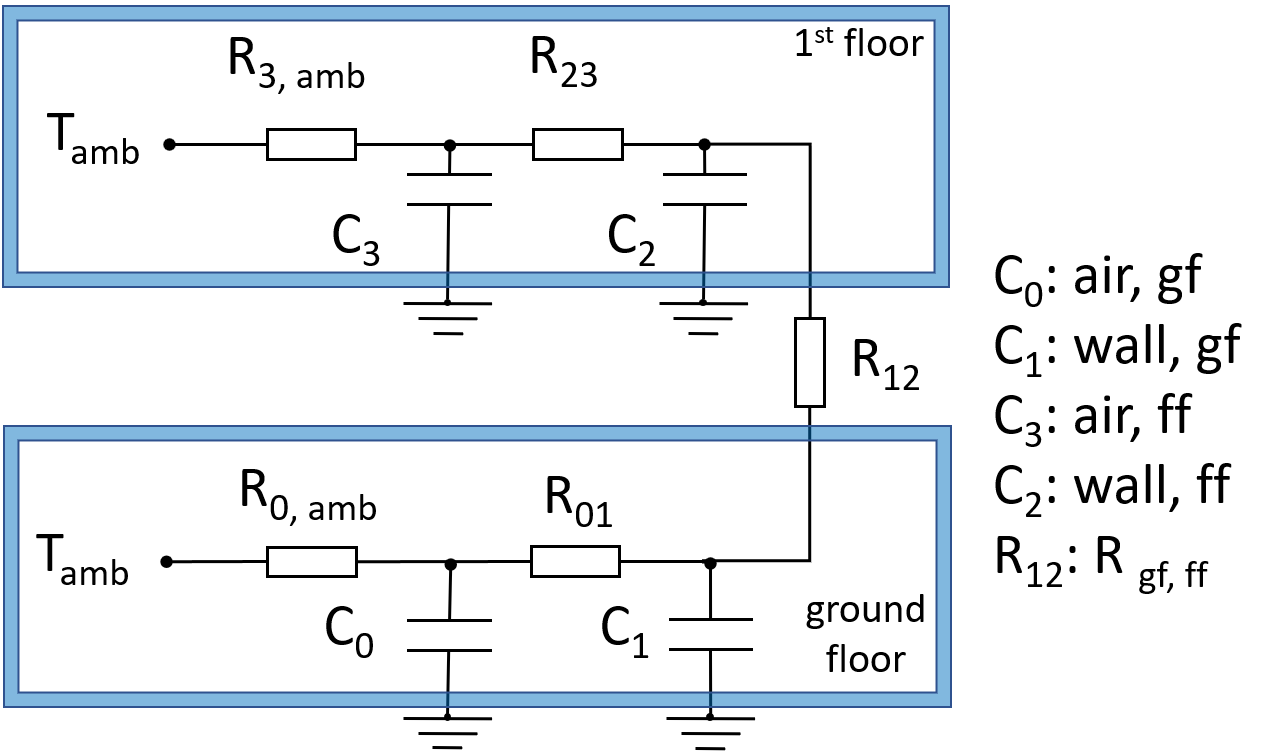
\includegraphics[width=0.6\columnwidth]{Pictures/5R4C_renumbered.png}
	\caption[Short title]{5R-4C house model, alternative representation, renumbered}
	\label{fig:renum5R4C}
\end{figure}

\begin{equation}
	\mathbf{C} \cdot \boldsymbol{\dot{\theta}} =
	\begin{bmatrix}
		C_{0} & 0 & 0 & 0\\
		0 &  C_{1} & 0 & 0 \\
		0 & 0 & C_{2} & 0\\
		0 & 0 & 0 & C_{3}
	\end{bmatrix}
	\cdot
	\begin{bmatrix}
		\frac{dT_{0}}{dt} \\
		\frac{dT_{1}}{dt} \\
		\frac{dT_{2}}{dt} \\
		\frac{dT_{3}}{dt} 
	\end{bmatrix}
\end{equation}

\begin{equation}
	\mathbf{K} \cdot \boldsymbol{\theta} =
	\begin{bmatrix}
		\frac{1}{R_{0, amb}} + \frac{1}{R_{01}} & \frac{-1}{R_{01}} & 0 & 0 \\
		\frac{-1}{R_{01}} &  \frac{1}{R_{01}} + \color{red}\frac{1}{R_{12}} & \color{red}\frac{-1}{R_{12}} & 0 \\
		0 & \color{red} \frac{-1}{R_{12}} & \frac{1}{R_{23}} + \color{red}\frac{1}{R_{12}}   & \frac{-1}{R_{23}}\\
		0 & 0 & \frac{-1}{R_{23}} &  \frac{1}{R_{3, amb}} + \frac{1}{R_{23}} \\
	\end{bmatrix}
	\cdot
	\begin{bmatrix}
		T_{0} \\
		T_{1} \\
		T_{2} \\
		T_{3}
	\end{bmatrix}
\end{equation}

\begin{equation}
	\mathbf{\dot{q}} =
	\begin{bmatrix}
		\frac{1}{R_{0, amb}} \cdot T_{amb} + \dot{Q}_{heat, 0} + \dot{Q}_{int, 0} + \dot{Q}_{solar, 0} \\
		\dot{Q}_{solar, 1} \\
		\dot{Q}_{solar, 2} \\
		\frac{1}{R_{3, amb}} \cdot T_{amb} + \dot{Q}_{heat, 3} + \dot{Q}_{int, 3} + \dot{Q}_{solar, 3}
	\end{bmatrix}
\end{equation}
		
\subsection{2R-2C model with buffervessel}

The "air" and "wall" nodes of the 2R2C model can be extended with "radiator" node. The radiator has a finite heat capacity of itself. Instead of a thermal resistance, the radiator heat exchange in $W/K$ is entered in the model. The radiator emits heat to the "air" node only. In its turn, the radiator is fed from a "buffervessel" node. The buffervessel loses heat to the radiator and is heated up by a gas boiler or alternatively a heat pump. The gas boiler does not heat the house directly, as was the case in the simplest model. A schematic view is given in Fig. \ref{fig:elecbuffer}.

\begin{figure}[H]
	\centering
	\includegraphics[width=0.7\columnwidth]{Pictures/buffervessel.png}
	\caption[Short title]{2R-2C house model with radiator and buffer vessel}
	\label{fig:buffervessel}
\end{figure} 

The differential equations for heat transport in the model of Fig. \ref{fig:elecbuffer} are:

\begin{equation}
	\begin{aligned}
	    C_{air} \frac{dT_{air}}{dt} &= \frac{T_{outdoor}-T_{air}}{R_{air_{\_}outdoor}} + \frac{T_{wall}-T_{air}}{R_{air_{\_}wall}} + U_{rad} \cdot A_{rad} \cdot (T_{return} - T_{air}) + \dot{Q}_{internal} + \dot{Q}_{solar, 0} \\
	    C_{wall} \frac{dT_{wall}}{dt} &= \frac{T_{air}-T_{wall}}{R_{air_{\_}wall}} + \dot{Q}_{solar, 1} \\
	    C_{rad} \frac{dT_{return}}{dt} &= \dot{m} \cdot c_{p, water} \cdot (T_{buffer} - T_{return}) + U_{rad} \cdot A_{rad} \cdot (T_{air} - T_{return}) \\
		C_{buffer} \frac{dT_{buffer}}{dt} &= \dot{m} \cdot c_{p, water} \cdot ( T_{return} - T_{buffer} ) + \dot{Q}_{inst} \\
	    \frac{dE}{dt} &= \dot{Q}_{inst}
	\end{aligned}
\end{equation}

 A fifth equation, integrating the heat source energy is sometimes added. Re-arranging the terms in the equation gives:
 
\begin{equation}
	\begin{aligned}
		C_{air} \frac{dT_{air}}{dt} &= \left[ \frac{-1}{R_{air_{\_}outdoor}} + \frac{-1}{R_{air_{\_}wall}} +  -1 \cdot U_{rad} \cdot A_{rad} \right] \cdot T_{air} + \frac{T_{wall}}{R_{air_{\_}wall}} + U_{rad} \cdot A_{rad} \cdot T_{return} + \\
		 & \frac{T_{outdoor}}{R_{air_{\_}outdoor}}  + \dot{Q}_{internal} + \dot{Q}_{solar, 0} \\
		C_{wall} \frac{dT_{wall}}{dt} &= \frac{1}{R_{air_{\_}wall}} \cdot T_{air} + \frac{-1}{R_{air_{\_}wall}} \cdot T_{wall} + \dot{Q}_{solar, 1} \\
		C_{rad} \frac{dT_{return}}{dt} &=  U_{rad} \cdot A_{rad} \cdot T_{air} + \left[- U_{rad} \cdot A_{rad} -\dot{m} \cdot c_{p, water}\right] \cdot T_{return} + \dot{m} \cdot c_{p, water} \cdot T_{buffer}\\
		C_{buffer} \frac{dT_{buffer}}{dt} &= \dot{m} \cdot c_{p, water} \cdot T_{return} - \dot{m} \cdot c_{p, water} \cdot T_{buffer} + \dot{Q}_{heat, 3} \\
		\frac{dE}{dt} &= \dot{Q}_{inst}
	\end{aligned}
\end{equation}
Conversion of the equations to a matrix equation yields:
\begin{equation}
	\mathbf{C} \cdot \boldsymbol{\dot{\theta}} =
	\begin{bmatrix}
		C_{0} & 0 & 0 & 0\\
		0 &  C_{1} & 0 & 0 \\
		0 & 0 & C_{2} & 0\\
		0 & 0 & 0 & C_{3}
	\end{bmatrix}
	\cdot
	\begin{bmatrix}
		\frac{dT_{0}}{dt} \\
		\frac{dT_{1}}{dt} \\
		\frac{dT_{2}}{dt} \\
		\frac{dT_{3}}{dt} 
	\end{bmatrix}
\end{equation}

\begin{equation}
	\mathbf{K} \cdot \boldsymbol{\theta} =
	\begin{bmatrix}
		\frac{1}{R_{0, amb}} + \frac{1}{R_{01}} + U \cdot A & \frac{-1}{R_{01}} & -U \cdot A & 0 \\
		\frac{-1}{R_{01}} &  \frac{1}{R_{01}}  & 0 & 0 \\
		-U \cdot A & 0 & U \cdot A + \frac{1}{R_{23}}  & \frac{-1}{R_{23}}\\
		0 & 0 & \frac{-1}{R_{23}} &  \frac{1}{R_{23}} \\
	\end{bmatrix}
	\cdot
	\begin{bmatrix}
		T_{0} \\
		T_{1} \\
		T_{2} \\
		T_{3}
	\end{bmatrix}
\end{equation}

\begin{equation}
	\mathbf{\dot{q}} =
	\begin{bmatrix}
		\frac{1}{R_{0, amb}} \cdot T_{amb} + \dot{Q}_{int, 0} + \dot{Q}_{solar, 0} \\
		\dot{Q}_{solar, 0} \\
		0 \\
		\dot{Q}_{heat, 3}
	\end{bmatrix}
\end{equation}

\subsection{2R-2C model with radiator only}

\begin{figure}[H]
	\centering
	\includegraphics[width=0.7\columnwidth]{Pictures/2R2C_radiator.png}
	\caption[Short title]{2R-2C house model with radiator only}
	\label{fig:2R2Cradiator}
\end{figure} 

The rate of heat transfer from a radiator to the ambient(room) air can be calculated as follows \cite{heatemissionrad}:

\begin{equation}
	\begin{aligned}
	    P & = P_{50} \cdot \left[\Delta T_{LMTD} \cdot \frac{1}{49.32}\right]^n \\
	    \Delta T_{LMTD} & = \frac{ T_{inlet} - T_{return} }{\ln \frac{ T_{inlet} - T_{ambient} }{T_{return} - T_{ambient}}} \\
	    n & = 1.33
    \end{aligned}
\end{equation}

This is sometimes simplified to:

\begin{equation}
	\begin{aligned}
		P & = U \cdot A \cdot \Delta T_{LMTD} \\
		\Delta T_{LMTD} & = \frac{ T_{inlet} - T_{return} }{\ln \frac{ T_{inlet} - T_{ambient} }{T_{return} - T_{ambient}}}
	\end{aligned}
\end{equation}

or simplified to \cite{NEN442, OEM442}:

\begin{equation}
	\begin{aligned}
		P & = K_m \cdot \Delta T^n \\
		\Delta T & = \frac{ T_{inlet} + T_{return} }{2} - {T_{ambient}}
	\end{aligned}
\end{equation}

The differential equations for heat transport in the model of Fig.~\ref{fig:2R2Cradiator} are:

\begin{equation}
	\begin{aligned}
		C_{air} \frac{dT_{air}}{dt} &= \frac{T_{outdoor}-T_{air}}{R_{air_{\_}outdoor}} + \frac{T_{wall}-T_{air}}{R_{air_{\_}wall}} + U_{rad} \cdot A_{rad} \cdot (T_{rad} - T_{air}) + \dot{Q}_{internal} + \dot{Q}_{solar, 0} \\
		C_{wall} \frac{dT_{wall}}{dt} &= \frac{T_{air}-T_{wall}}{R_{air_{\_}wall}} + \dot{Q}_{solar, 1} \\
		C_{rad} \frac{dT_{rad}}{dt} &= \dot{Q}_{inst} + U_{rad} \cdot A_{rad} \cdot (T_{air} - T_{rad}) \\
	\end{aligned}
\end{equation}

Re-arranging the terms in the equation gives:

\begin{equation}
	\begin{aligned}
		C_{air} \frac{dT_{air}}{dt} &= \left[ \frac{-1}{R_{air_{\_}outdoor}} + \frac{-1}{R_{air_{\_}wall}} +  -1 \cdot U_{rad} \cdot A_{rad} \right] \cdot T_{air} + \frac{T_{wall}}{R_{air_{\_}wall}} +  U_{rad} \cdot A_{rad} \cdot T_{rad} + \\
		& \frac{T_{outdoor}}{R_{air_{\_}outdoor}}  + \dot{Q}_{internal} + \dot{Q}_{solar, 0} \\
		C_{wall} \frac{dT_{wall}}{dt} &= \frac{1}{R_{air_{\_}wall}} \cdot T_{air} + \frac{-1}{R_{air_{\_}wall}} \cdot T_{wall} + \dot{Q}_{solar, 1} \\
		C_{rad} \frac{dT_{rad}}{dt} &=  U_{rad} \cdot A_{rad} \cdot T_{air} - U_{rad} \cdot A_{rad} \cdot T_{rad} + \dot{Q}_{heat, 2}\\
	\end{aligned}
\end{equation}
Conversion of the equations to a matrix equation yields:
\begin{equation}
	\mathbf{C} \cdot \boldsymbol{\dot{\theta}} =
	\begin{bmatrix}
		C_{0} & 0 & 0 \\
		0 &  C_{1} & 0  \\
		0 & 0 & C_{2} 
	\end{bmatrix}
	\cdot
	\begin{bmatrix}
		\frac{dT_{0}}{dt} \\
		\frac{dT_{1}}{dt} \\
		\frac{dT_{2}}{dt} 
	\end{bmatrix}
\end{equation}

\begin{equation}
	\mathbf{K} \cdot \boldsymbol{\theta} =
	\begin{bmatrix}
		\frac{1}{R_{0, amb}} + \frac{1}{R_{01}} + U \cdot A & \frac{-1}{R_{01}} & -U \cdot A  \\
		\frac{-1}{R_{01}} &  \frac{1}{R_{01}}  & 0  \\
		-U \cdot A & 0 & U \cdot A 
	\end{bmatrix}
	\cdot
	\begin{bmatrix}
		T_{0} \\
		T_{1} \\
		T_{2}
	\end{bmatrix}
\end{equation}

\begin{equation}
	\mathbf{\dot{q}} =
	\begin{bmatrix}
		\frac{1}{R_{0, amb}} \cdot T_{amb} + \dot{Q}_{int, 0} + \dot{Q}_{solar, 0} \\
		\dot{Q}_{solar, 1} \\
		\dot{Q}_{heat, 2}
	\end{bmatrix}
\end{equation}


\begin{figure}[H]
	\centering
	\includegraphics[width=0.7\columnwidth]{Pictures/2R2C_radiator_chains.png}
	\caption[Short title]{2R-2C house model with radiator in 3 chains}
	\label{fig:2R2Cradiator_chains}
\end{figure} 

Starting with the basic 2R2C model we write down the matrices. Note that the heat source for the house is omitted at first. Solar energy entering the house is partitioned between air and wall, Heat generated due to the presence and activities of inhabitants is added to the air node:

\begin{equation}
	\mathbf{C} \cdot \boldsymbol{\dot{\theta}} =
	\begin{bmatrix}
		C_{0} & 0 \\
		0 &  C_{1}
	\end{bmatrix}
	\cdot
	\begin{bmatrix}
		\frac{dT_{0}}{dt} \\
		\frac{dT_{1}}{dt}
	\end{bmatrix}
\end{equation}

\begin{equation}
	\mathbf{K} \cdot \boldsymbol{\theta} =
	\begin{bmatrix}
		\frac{1}{R_{0, amb}} + \frac{1}{R_{01}} & \frac{-1}{R_{01}} \\
		\frac{-1}{R_{01}} &  \frac{1}{R_{01}}
	\end{bmatrix}
	\cdot
	\begin{bmatrix}
		T_{0} \\
		T_{1}
	\end{bmatrix}
\end{equation}

\begin{equation}
	\mathbf{\dot{q}} =
	\begin{bmatrix}
		\frac{1}{R_{0, amb}} \cdot T_{amb} + \dot{Q}_{int, 0} + \dot{Q}_{solar, 0} \\
		\dot{Q}_{solar, 1}
	\end{bmatrix}
\end{equation}

As a third link in the chain, a radiator is added, with a heat capacity $C_{rad}$ and a heat delivery $U \cdot A \cdot (T_{rad} - T_{air})$ to the air node. The heat source $\dot{Q}_{inst}$ is now connected to the radiator.

\begin{equation}
	\mathbf{C} \cdot \boldsymbol{\dot{\theta}} =
	\begin{bmatrix}
		C_{0} & 0 & \color{red} 0 \\
		0 &  C_{1} & \color{red} 0  \\
		\color{red} 0 & \color{red} 0 & \color{red} C_{2} 
	\end{bmatrix}
	\cdot
	\begin{bmatrix}
		\frac{dT_{0}}{dt} \\
		\frac{dT_{1}}{dt} \\
		\color{red}\frac{dT_{2}}{dt} 
	\end{bmatrix}
\end{equation}

\begin{equation}
	\mathbf{K} \cdot \boldsymbol{\theta} =
	\begin{bmatrix}
		\frac{1}{R_{0, amb}} + \frac{1}{R_{01}} {\color{red}+ U \cdot A} & \frac{-1}{R_{01}} & {\color{red}-U \cdot A}  \\
		\frac{-1}{R_{01}} &  \frac{1}{R_{01}}  & \color{red} 0  \\
		{\color{red}-U \cdot A} & \color{red} 0 & {\color{red}U \cdot A }
	\end{bmatrix}
	\cdot
	\begin{bmatrix}
		T_{0} \\
		T_{1} \\
	   \color{red}T_{2}
	\end{bmatrix}
\end{equation}

\begin{equation}
	\mathbf{\dot{q}} =
	\begin{bmatrix}
		\frac{1}{R_{0, amb}} \cdot T_{amb} + \dot{Q}_{int, 0} + \dot{Q}_{solar, 0} \\
		\dot{Q}_{solar, 1} \\
		\color{red} \dot{Q}_{heat, 2}
	\end{bmatrix}
\end{equation}

In this example, it becomes visible (in red) that the rank of the $C$- and $K$-matrix, and the $\dot{q}$-vector is extended by 1. The heat capacity of the radiator is included as an extra \emph{diagonal} element in the $C$-matrix. The heat delivery from the radiator to the indoor air is added to or subtracted from the {00}, {22}, {02} and {20} elements of th $K$-matrix, so that it remains a \emph{symmetric} matrix. The heater is connected to the radiator, represented by element {2} of the $\dot{q}$-vector. 
%\usepackage{xcolor}

\subsection{2R2C revisited: 2R3C}
The 2R2C model as represented in \ref{fig:elec2R2C} treats the node of the outside temperature ($T_{amb}$) differently from the other nodes, $T_{air}$ and $T_{walls}$.  This representation is inconsistent, and actually incomplete. Implicitly, the model links a source/sink to the node that controls the outdoor temperature. In literature, one can find models in which this source has been made explicit, such as in \cite{achterbos}. It seems that this representation has been lost over time. 

In order to complete the analogy with the other nodes in the model we can connect an additional capacitor ($C_amb$). The capacity will be tending to infinity, as we assume the outside temperature not to change due to heat exchange with the house.

\todo{todo:figure including a source and capacitor}

Adding the capacitor and the source also will change the equations. Actually, it results in a more structured set of equations. The equations will be as follows:
\begin{equation}
	\mathbf{C} \cdot \boldsymbol{\dot{\theta}} =
	\begin{bmatrix}
		C_{amb} & 0 & 0\\
		0 &  C_{air} & 0   \\
		0 & 0 & C_{wall} 
	\end{bmatrix}
	\cdot
	\begin{bmatrix}
		\frac{dT_{amb}}{dt} \\
		\frac{dT_{air}}{dt} \\
		\frac{dT_{wall}}{dt} 
	\end{bmatrix}
\end{equation}

\begin{equation}
	\mathbf{K} \cdot \boldsymbol{\theta} =
	\begin{bmatrix}
		\frac{1}{R_{0, amb}}  & \frac{-1}{R_{amb,air}} & 0  \\
		\frac{-1}{R_{amb, air}} &  \frac{1}{R_{01}} + \frac{1}{R_{air,wall}} &  \frac{-1}{R_{air,wall}} \\
		 0 & \frac{-1}{R_{air, wall}}  & \frac{1}{R_{air,wall}} 
	\end{bmatrix}
	\cdot
	\begin{bmatrix}
		T_{amb} \\
		T_{air} \\
		T_{wall}
	\end{bmatrix}
\end{equation}

\begin{equation}
	\mathbf{\dot{q}} =
	\begin{bmatrix}
		\dot{Q}_{amb}\\
		\dot{Q}_{air} \\
		\dot{Q}_{wall} 
	\end{bmatrix}
\end{equation}

In the equations we now see that the matrix $K$ represents the interaction between the different heat capacitors. The structure of $K$ is such that the sum over the rows will always be zero, where the diagonal elements equal the negative sum of the off-diagonal elements. The off-diagonal elements are equal to (minus) conductance factor $\frac{-1}{R}$ between the respective connected nodes. 

The vector $\dot{q}$ contains all heat sources (and sinks). 

Generalizing the idea above, alternative models can be easily constructed using a graph. In the graph each node is labelled with a heat capacity $C_i$, and temperature $T_i$. Nodes $i$ and $j$ can be connected by an edge labelled with $R_{i,j}$, where $\frac{1}{R_{i,j}}$ represents the heat conductance between the two nodes. The $K$-matrix is the connectivity matrix of the graph, where $K_{i,j} = \frac{-1}{R_{i,j}}$. The diagonal elements, $K{i,i}$ are set such that the sums over the rows will be equal to zero.
 

Additionally, each node can be connected to a source or sink. The heat generated or absorbed at each node will be added through the vector $\dot{q}$.

\subsubsection{example: 2R-2C house with buffer}

   


\subsection{Package "housemodel"}

The repository "\textsf{twozone\_housemodel-git}" contains the modules for the house model. The customary way to organize the modules is to make a \emph{Python package} with \emph{subpackages}. This opens up the possibility of publishing the package on PyPi, so that it can be imported.

See: \url{https://pypi.org/}

From commit \textsf{e74ce58} the files in the \textsf{twozone\_housemodel-git} repository are organized as a package. The proposed structure, implemented in this commit, is:

\dirtree{%
	.1 twozone\_housemodel-git.
	.2 housemodel.
	.3 \_\_init\_\_.py.
	.3 controls.
	.4 \_\_init\_\_.py.
	.3 solvers.
	.4 \_\_init\_\_.py.
	.3 sourcesink.
	.4 \_\_init\_\_.py.
	.3 tools.
	.4 \_\_init\_\_.py.
	.2 tests.
	.3 \_\_init\_\_.py.
	.3 context1.py.
	.3 test\_*.py.
} 

\begin{itemize}
	\item the \emph{repository root} \textsf{twozone\_housemodel-git} contains the simulation scripts and configuration files (for now) 
	\item the \emph{package root} \textsf{housemodel} contains the complete package. This can be seen since it contains an (empty) \textsf{\_\_init\_\_.py} module.
	\item the \emph{subpackage} folders contain the modules with common functions and classes for all simulations. They each contain an (empty) \textsf{\_\_init\_\_.py} module.
	\item a \textsf{tests} folder is placed carefully as a subfolder of the \emph{repository root}. 
	See: \url{https://docs.python-guide.org/writing/structure/} for the underlying philosophy. Here, testing modules (scripts) can be placed. If the names of the test scripts start with \textsf{test\_}, they can be automatically run with the \textsf{pytest} Python package.
\end{itemize}

\textit{Note}: Running the simulations and tests is best done from the \emph{repository root}. All simulations and tests have been updated to find the package, subpackages and configuration files from this directory.

\section{Thermal model of a building with installations}

\subsection{2R-2C model with buffervessel}

The "air" and "wall" nodes of the 2R2C model can be extended with "radiator" node. The radiator has a finite heat capacity of itself. Instead of a thermal resistance, the radiator heat exchange in $W/K$ is entered in the model. The radiator emits heat to the "air" node only. In its turn, the radiator is fed from a "buffervessel" node. The buffervessel loses heat to the radiator and is heated up by a gas boiler or alternatively a heat pump. The gas boiler does not heat the house directly, as was the case in the simplest model. A schematic view is given in Fig. \ref{fig:elecbuffer}.

\begin{figure}[H]
	\centering
	\includegraphics[width=0.7\columnwidth]{Figures/buffervessel.png}
	\caption[Short title]{2R-2C house model with radiator and buffer vessel}
	\label{fig:buffervessel}
\end{figure} 

The differential equations for heat transport in the model of Fig. \ref{fig:elecbuffer} are:

\begin{equation}
	\begin{aligned}
	    C_{air} \frac{dT_{air}}{dt} &= \frac{T_{outdoor}-T_{air}}{R_{air_{\_}outdoor}} + \frac{T_{wall}-T_{air}}{R_{air_{\_}wall}} + U_{rad} \cdot A_{rad} \cdot (T_{return} - T_{air}) + \dot{Q}_{internal} + \dot{Q}_{solar, 0} \\
	    C_{wall} \frac{dT_{wall}}{dt} &= \frac{T_{air}-T_{wall}}{R_{air_{\_}wall}} + \dot{Q}_{solar, 1} \\
	    C_{rad} \frac{dT_{return}}{dt} &= \dot{m} \cdot c_{p, water} \cdot (T_{buffer} - T_{return}) + U_{rad} \cdot A_{rad} \cdot (T_{air} - T_{return}) \\
		C_{buffer} \frac{dT_{buffer}}{dt} &= \dot{m} \cdot c_{p, water} \cdot ( T_{return} - T_{buffer} ) + \dot{Q}_{inst} \\
	    \frac{dE}{dt} &= \dot{Q}_{inst}
	\end{aligned}
\end{equation}

 A fifth equation, integrating the heat source energy is sometimes added. Re-arranging the terms in the equation gives:
 
\begin{equation}
	\begin{aligned}
		C_{air} \frac{dT_{air}}{dt} &= \left[ \frac{-1}{R_{air_{\_}outdoor}} + \frac{-1}{R_{air_{\_}wall}} +  -1 \cdot U_{rad} \cdot A_{rad} \right] \cdot T_{air} + \frac{T_{wall}}{R_{air_{\_}wall}} + U_{rad} \cdot A_{rad} \cdot T_{return} + \\
		 & \frac{T_{outdoor}}{R_{air_{\_}outdoor}}  + \dot{Q}_{internal} + \dot{Q}_{solar, 0} \\
		C_{wall} \frac{dT_{wall}}{dt} &= \frac{1}{R_{air_{\_}wall}} \cdot T_{air} + \frac{-1}{R_{air_{\_}wall}} \cdot T_{wall} + \dot{Q}_{solar, 1} \\
		C_{rad} \frac{dT_{return}}{dt} &=  U_{rad} \cdot A_{rad} \cdot T_{air} + \left[- U_{rad} \cdot A_{rad} -\dot{m} \cdot c_{p, water}\right] \cdot T_{return} + \dot{m} \cdot c_{p, water} \cdot T_{buffer}\\
		C_{buffer} \frac{dT_{buffer}}{dt} &= \dot{m} \cdot c_{p, water} \cdot T_{return} - \dot{m} \cdot c_{p, water} \cdot T_{buffer} + \dot{Q}_{heat, 3} \\
		\frac{dE}{dt} &= \dot{Q}_{inst}
	\end{aligned}
\end{equation}
Conversion of the equations to a matrix equation yields:
\begin{equation}
	\mathbf{C} \cdot \boldsymbol{\dot{\theta}} =
	\begin{bmatrix}
		C_{0} & 0 & 0 & 0\\
		0 &  C_{1} & 0 & 0 \\
		0 & 0 & C_{2} & 0\\
		0 & 0 & 0 & C_{3}
	\end{bmatrix}
	\cdot
	\begin{bmatrix}
		\frac{dT_{0}}{dt} \\
		\frac{dT_{1}}{dt} \\
		\frac{dT_{2}}{dt} \\
		\frac{dT_{3}}{dt} 
	\end{bmatrix}
\end{equation}

\begin{equation}
	\mathbf{K} \cdot \boldsymbol{\theta} =
	\begin{bmatrix}
		\frac{1}{R_{0, amb}} + \frac{1}{R_{01}} + U \cdot A & \frac{-1}{R_{01}} & -U \cdot A & 0 \\
		\frac{-1}{R_{01}} &  \frac{1}{R_{01}}  & 0 & 0 \\
		-U \cdot A & 0 & U \cdot A + \frac{1}{R_{23}}  & \frac{-1}{R_{23}}\\
		0 & 0 & \frac{-1}{R_{23}} &  \frac{1}{R_{23}} \\
	\end{bmatrix}
	\cdot
	\begin{bmatrix}
		T_{0} \\
		T_{1} \\
		T_{2} \\
		T_{3}
	\end{bmatrix}
\end{equation}

\begin{equation}
	\mathbf{\dot{q}} =
	\begin{bmatrix}
		\frac{1}{R_{0, amb}} \cdot T_{amb} + \dot{Q}_{int, 0} + \dot{Q}_{solar, 0} \\
		\dot{Q}_{solar, 0} \\
		0 \\
		\dot{Q}_{heat, 3}
	\end{bmatrix}
\end{equation}

\subsection{2R-2C model with radiator only}

\begin{figure}[H]
	\centering
	\includegraphics[width=0.7\columnwidth]{Figures/2R2C_radiator.png}
	\caption[Short title]{2R-2C house model with radiator only}
	\label{fig:2R2Cradiator}
\end{figure} 

The rate of heat transfer from a radiator to the ambient(room) air can be calculated as follows \cite{heatemissionrad}:

\begin{equation}
	\begin{aligned}
	    P & = P_{50} \cdot \left[\Delta T_{LMTD} \cdot \frac{1}{49.32}\right]^n \\
	    \Delta T_{LMTD} & = \frac{ T_{inlet} - T_{return} }{\ln \frac{ T_{inlet} - T_{ambient} }{T_{return} - T_{ambient}}} \\
	    n & = 1.33
    \end{aligned}
\end{equation}

This is sometimes simplified to:

\begin{equation}
	\begin{aligned}
		P & = U \cdot A \cdot \Delta T_{LMTD} \\
		\Delta T_{LMTD} & = \frac{ T_{inlet} - T_{return} }{\ln \frac{ T_{inlet} - T_{ambient} }{T_{return} - T_{ambient}}}
	\end{aligned}
\end{equation}

or simplified to \cite{NEN442, OEM442}:

\begin{equation}
	\begin{aligned}
		P & = K_m \cdot \Delta T^n \\
		\Delta T & = \frac{ T_{inlet} + T_{return} }{2} - {T_{ambient}}
	\end{aligned}
\end{equation}

The differential equations for heat transport in the model of Fig.~\ref{fig:2R2Cradiator} are:

\begin{equation}
	\begin{aligned}
		C_{air} \frac{dT_{air}}{dt} &= \frac{T_{outdoor}-T_{air}}{R_{air_{\_}outdoor}} + \frac{T_{wall}-T_{air}}{R_{air_{\_}wall}} + U_{rad} \cdot A_{rad} \cdot (T_{rad} - T_{air}) + \dot{Q}_{internal} + \dot{Q}_{solar, 0} \\
		C_{wall} \frac{dT_{wall}}{dt} &= \frac{T_{air}-T_{wall}}{R_{air_{\_}wall}} + \dot{Q}_{solar, 1} \\
		C_{rad} \frac{dT_{rad}}{dt} &= \dot{Q}_{inst} + U_{rad} \cdot A_{rad} \cdot (T_{air} - T_{rad}) \\
	\end{aligned}
\end{equation}

Re-arranging the terms in the equation gives:

\begin{equation}
	\begin{aligned}
		C_{air} \frac{dT_{air}}{dt} &= \left[ \frac{-1}{R_{air_{\_}outdoor}} + \frac{-1}{R_{air_{\_}wall}} +  -1 \cdot U_{rad} \cdot A_{rad} \right] \cdot T_{air} + \frac{T_{wall}}{R_{air_{\_}wall}} +  U_{rad} \cdot A_{rad} \cdot T_{rad} + \\
		& \frac{T_{outdoor}}{R_{air_{\_}outdoor}}  + \dot{Q}_{internal} + \dot{Q}_{solar, 0} \\
		C_{wall} \frac{dT_{wall}}{dt} &= \frac{1}{R_{air_{\_}wall}} \cdot T_{air} + \frac{-1}{R_{air_{\_}wall}} \cdot T_{wall} + \dot{Q}_{solar, 1} \\
		C_{rad} \frac{dT_{rad}}{dt} &=  U_{rad} \cdot A_{rad} \cdot T_{air} - U_{rad} \cdot A_{rad} \cdot T_{rad} + \dot{Q}_{heat, 2}\\
	\end{aligned}
\end{equation}
Conversion of the equations to a matrix equation yields:
\begin{equation}
	\mathbf{C} \cdot \boldsymbol{\dot{\theta}} =
	\begin{bmatrix}
		C_{0} & 0 & 0 \\
		0 &  C_{1} & 0  \\
		0 & 0 & C_{2} 
	\end{bmatrix}
	\cdot
	\begin{bmatrix}
		\frac{dT_{0}}{dt} \\
		\frac{dT_{1}}{dt} \\
		\frac{dT_{2}}{dt} 
	\end{bmatrix}
\end{equation}

\begin{equation}
	\mathbf{K} \cdot \boldsymbol{\theta} =
	\begin{bmatrix}
		\frac{1}{R_{0, amb}} + \frac{1}{R_{01}} + U \cdot A & \frac{-1}{R_{01}} & -U \cdot A  \\
		\frac{-1}{R_{01}} &  \frac{1}{R_{01}}  & 0  \\
		-U \cdot A & 0 & U \cdot A 
	\end{bmatrix}
	\cdot
	\begin{bmatrix}
		T_{0} \\
		T_{1} \\
		T_{2}
	\end{bmatrix}
\end{equation}

\begin{equation}
	\mathbf{\dot{q}} =
	\begin{bmatrix}
		\frac{1}{R_{0, amb}} \cdot T_{amb} + \dot{Q}_{int, 0} + \dot{Q}_{solar, 0} \\
		\dot{Q}_{solar, 1} \\
		\dot{Q}_{heat, 2}
	\end{bmatrix}
\end{equation}


\begin{figure}[H]
	\centering
	\includegraphics[width=0.7\columnwidth]{Figures/2R2C_radiator_chains.png}
	\caption[Short title]{2R-2C house model with radiator in 3 chains}
	\label{fig:2R2Cradiator_chains}
\end{figure} 

Starting with the basic 2R2C model we write down the matrices. Note that the heat source for the house is omitted at first. Solar energy entering the house is partitioned between air and wall, Heat generated due to the presence and activities of inhabitants is added to the air node:

\begin{equation}
	\mathbf{C} \cdot \boldsymbol{\dot{\theta}} =
	\begin{bmatrix}
		C_{0} & 0 \\
		0 &  C_{1}
	\end{bmatrix}
	\cdot
	\begin{bmatrix}
		\frac{dT_{0}}{dt} \\
		\frac{dT_{1}}{dt}
	\end{bmatrix}
\end{equation}

\begin{equation}
	\mathbf{K} \cdot \boldsymbol{\theta} =
	\begin{bmatrix}
		\frac{1}{R_{0, amb}} + \frac{1}{R_{01}} & \frac{-1}{R_{01}} \\
		\frac{-1}{R_{01}} &  \frac{1}{R_{01}}
	\end{bmatrix}
	\cdot
	\begin{bmatrix}
		T_{0} \\
		T_{1}
	\end{bmatrix}
\end{equation}

\begin{equation}
	\mathbf{\dot{q}} =
	\begin{bmatrix}
		\frac{1}{R_{0, amb}} \cdot T_{amb} + \dot{Q}_{int, 0} + \dot{Q}_{solar, 0} \\
		\dot{Q}_{solar, 1}
	\end{bmatrix}
\end{equation}

As a third link in the chain, a radiator is added, with a heat capacity $C_{rad}$ and a heat delivery $U \cdot A \cdot (T_{rad} - T_{air})$ to the air node. The heat source $\dot{Q}_{inst}$ is now connected to the radiator.

\begin{equation}
	\mathbf{C} \cdot \boldsymbol{\dot{\theta}} =
	\begin{bmatrix}
		C_{0} & 0 & \color{red} 0 \\
		0 &  C_{1} & \color{red} 0  \\
		\color{red} 0 & \color{red} 0 & \color{red} C_{2} 
	\end{bmatrix}
	\cdot
	\begin{bmatrix}
		\frac{dT_{0}}{dt} \\
		\frac{dT_{1}}{dt} \\
		\color{red}\frac{dT_{2}}{dt} 
	\end{bmatrix}
\end{equation}

\begin{equation}
	\mathbf{K} \cdot \boldsymbol{\theta} =
	\begin{bmatrix}
		\frac{1}{R_{0, amb}} + \frac{1}{R_{01}} {\color{red}+ U \cdot A} & \frac{-1}{R_{01}} & {\color{red}-U \cdot A}  \\
		\frac{-1}{R_{01}} &  \frac{1}{R_{01}}  & \color{red} 0  \\
		{\color{red}-U \cdot A} & \color{red} 0 & {\color{red}U \cdot A }
	\end{bmatrix}
	\cdot
	\begin{bmatrix}
		T_{0} \\
		T_{1} \\
	   \color{red}T_{2}
	\end{bmatrix}
\end{equation}

\begin{equation}
	\mathbf{\dot{q}} =
	\begin{bmatrix}
		\frac{1}{R_{0, amb}} \cdot T_{amb} + \dot{Q}_{int, 0} + \dot{Q}_{solar, 0} \\
		\dot{Q}_{solar, 1} \\
		\color{red} \dot{Q}_{heat, 2}
	\end{bmatrix}
\end{equation}

In this example, it becomes visible (in red) that the rank of the $C$- and $K$-matrix, and the $\dot{q}$-vector is extended by 1. The heat capacity of the radiator is included as an extra \emph{diagonal} element in the $C$-matrix. The heat delivery from the radiator to the indoor air is added to or subtracted from the {00}, {22}, {02} and {20} elements of th $K$-matrix, so that it remains a \emph{symmetric} matrix. The heater is connected to the radiator, represented by element {2} of the $\dot{q}$-vector. 
%\usepackage{xcolor}

\subsection{2R2C revisited: 2R3C}
\label{sec:2R3C}
The 2R2C model as represented in \ref{fig:elec2R2C} treats the node of the outside temperature ($T_{amb}$) differently from the other nodes, $T_{air}$ and $T_{walls}$.  This representation is inconsistent, and actually incomplete. Implicitly, the model links a source/sink to the node that controls the outdoor temperature. In literature, one can find models in which this source has been made explicit, such as in \cite{achterbos}. It seems that this representation has been lost over time. 

In order to complete the analogy with the other nodes in the model we can connect an additional capacitor ($C_{amb}$). The capacity will be tending to infinity, as we assume the outside temperature does not  change due to heat exchange with the house.

\todo{todo:figure including a source and capacitor}

Adding the capacitor and the source also will change the equations. Actually, it results in a more structured set of equations. The equations will be as follows:
\begin{equation}
	\mathbf{C} \cdot \boldsymbol{\dot{\theta}} =
	\begin{bmatrix}
		C_{amb} & 0 & 0\\
		0 &  C_{air} & 0   \\
		0 & 0 & C_{wall} 
	\end{bmatrix}
	\cdot
	\begin{bmatrix}
		\frac{dT_{amb}}{dt} \\
		\frac{dT_{air}}{dt} \\
		\frac{dT_{wall}}{dt} 
	\end{bmatrix}
\end{equation}

\begin{equation}
	\mathbf{K} \cdot \boldsymbol{\theta} =
	\begin{bmatrix}
		\frac{1}{R_{amb, air}}  & \frac{-1}{R_{amb,air}} & 0  \\
		\frac{-1}{R_{amb, air}} &  \frac{1}{R_{amb, air}} + \frac{1}{R_{air,wall}} &  \frac{-1}{R_{air,wall}} \\
		 0 & \frac{-1}{R_{air, wall}}  & \frac{1}{R_{air,wall}} 
	\end{bmatrix}
	\cdot
	\begin{bmatrix}
		T_{amb} \\
		T_{air} \\
		T_{wall}
	\end{bmatrix}
\end{equation}

\begin{equation}
	\mathbf{\dot{q}} =
	\begin{bmatrix}
		\dot{Q}_{amb}\\
		\dot{Q}_{air} \\
		\dot{Q}_{wall} 
	\end{bmatrix}
\end{equation}

In the equations we now see that the matrix $K$ represents the interaction between the different heat capacities.  The off-diagonal elements are equal to (minus) conductance factor $\frac{-1}{R}$ between the respective connected nodes. The structure of $K$ is such that the sum over the rows will always be zero, where the diagonal elements equal the negative sum of the off-diagonal elements.

The vector $\dot{q}$ contains all heat sources (and sinks). 

Generalizing the idea above, alternative models can be easily constructed using an underlying graph. In the graph each node is labeled with a heat capacity $C_i$, and temperature $T_i$. Nodes $i$ and $j$ can be connected by an edge labeled with $R_{i,j}$, where $\frac{1}{R_{i,j}}$ represents the heat conductance between the two nodes. The $K$-matrix is the connectivity matrix of the graph, where $K_{i,j} = \frac{-1}{R_{i,j}}$. The diagonal elements, $K{i,i}$ are set such that the sums over the rows will be equal to zero.
 

Additionally, each node can be connected to a source (or sink). Two types of sources are available. A "temperature source" represents a source that will keep the temperature of the connected node constant. This source type can be used to set the ambient temperature.   

A heat source represents a source that will provide a continuous constant energy flow into the node. This source type can be used to represent the inflow of energy by for example the sun. 

\subsubsection{example: 2R-2C house with buffer}

   
\subsection{3R2C model}

For an apartment building, the simplest model has two nodes with a finite heat capacity, the interior and the building construction. Both nodes have a finite thermal resistance to the ambient environment. Finally there is a thermal resistance between the nodes. Graphically, the model is represented by Figure~\ref{fig:3R2C}

\begin{figure}[H]
	\centering
	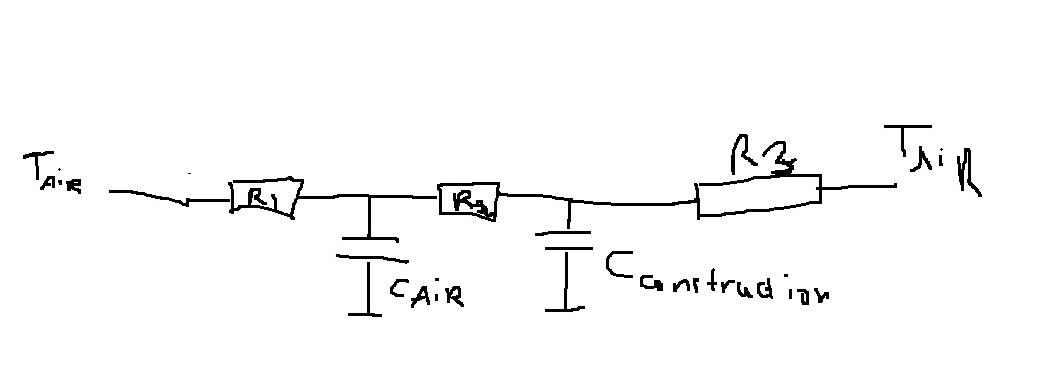
\includegraphics[width=0.7\columnwidth]{Figures/3R2Cmodel}
	\caption[Short title]{3R-2C house model}
	\label{fig:3R2C}
\end{figure} 

The differential equations are:

\begin{equation}
	\begin{aligned}
		C_{air}\frac{dT_{air}}{dt} &=\frac{T_{amb}-T_{air}}{R_{air, amb}} + \frac{T_{wall}-T_{air}}{R_{air, wall}} + \dot{Q}_{heat, air} + \dot{Q}_{int, air} + \dot{Q}_{solar, air} 
		\\ \\
		C_{wall}\frac{dT_{wall}}{dt} &=\frac{T_{air}-T_{wall}}{R_{air, wall}} + \frac{T_{amb}-T_{wall}}{R_{wall, amb}} +\dot{Q}_{solar, wall}
	\end{aligned}
\end{equation}

Writing out the differential equations in the classical notation:

\begin{equation}
	\begin{aligned}
		C_{air}\frac{dT_{air}}{dt} &= \left[ \frac{-1}{R_{air, amb}} + \frac{-1}{R_{air, wall}} \right]  \cdot T_{air}  + \frac{1}{R_{air, wall}} \cdot T_{wall} + \frac{1}{R_{air, amb}} \cdot T_{amb} + \dot{Q}_{heat, air} + \dot{Q}_{int, air} + \dot{Q}_{solar, air} 
		\\ \\
		C_{wall}\frac{dT_{wall}}{dt} &= \frac{1}{R_{air, wall}} \cdot T_{air} + \left[ \frac{-1}{R_{wall, amb}} + \frac{-1}{R_{air, wall}} \right]  \cdot T_{wall} + \frac{1}{R_{wall, amb}} \cdot T_{amb} + \dot{Q}_{solar, wall}
	\end{aligned}
\end{equation}

The differential equations can be written in matrix notation as:

\begin{subequations}
	\label{eq:matnot}
	\begin{align}
		\mathbf{C} \cdot \boldsymbol{\dot{\theta}} = - \mathbf{K} \cdot \boldsymbol{\theta} + \mathbf{\dot{q}} \\ 
		\mathbf{C} \cdot \boldsymbol{\dot{\theta}} + \mathbf{K} \cdot \boldsymbol{\theta} = \mathbf{\dot{q}}
	\end{align}
\end{subequations}

with:

\begin{equation}
	\mathbf{C} \cdot \boldsymbol{\dot{\theta}} =
	\begin{bmatrix}
		C_{air} & 0 \\
		0 &  C_{wall}
	\end{bmatrix}
	\cdot
	\begin{bmatrix}
		\frac{dT_{air}}{dt} \\
		\frac{dT_{wall}}{dt}
	\end{bmatrix}
\end{equation}

\begin{equation}
	\mathbf{K} \cdot \boldsymbol{\theta} =
	\begin{bmatrix}
		\frac{1}{R_{air, amb}} + \frac{1}{R_{air, wall}} & \frac{-1}{R_{air, wall}} \\
		\frac{-1}{R_{air, wall}} &  \frac{1}{R_{wall, amb}} + \frac{1}{R_{air, wall}}
	\end{bmatrix}
	\cdot
	\begin{bmatrix}
		T_{air} \\
		T_{wall}
	\end{bmatrix}
\end{equation}

\begin{equation}
	\mathbf{\dot{q}} =
	\begin{bmatrix}
		\frac{1}{R_{air, amb}} \cdot T_{amb} + \dot{Q}_{heat, air} + \dot{Q}_{int, air} + \dot{Q}_{solar, air} \\
		\frac{1}{R_{wall, amb}} \cdot T_{amb} + \dot{Q}_{solar, wall}
	\end{bmatrix}
\end{equation}

Written out, the differential equation according to \eqref{eq:matnot} becomes:

\begin{equation}
	\begin{aligned}
		\begin{bmatrix}
			C_{air} & 0 \\
			0 &  C_{wall}
		\end{bmatrix}
		\cdot
		\begin{bmatrix}
			\frac{dT_{air}}{dt} \\
			\frac{dT_{wall}}{dt}
		\end{bmatrix}
		=
		\begin{bmatrix}
			\frac{-1}{R_{air, amb}} + \frac{-1}{R_{air, wall}} & \frac{1}{R_{air, wall}} \\
			\frac{1}{R_{air, wall}} &  \frac{-1}{R_{wall, amb}} + \frac{-1}{R_{air, wall}}
		\end{bmatrix}
		\cdot
		\begin{bmatrix}
			T_{air} \\
			T_{wall}
		\end{bmatrix}
		+ \\ \\
		\begin{bmatrix}
			\frac{1}{R_{air, amb}} \cdot T_{amb} + \dot{Q}_{heat, air} + \dot{Q}_{int, air} + \dot{Q}_{solar, air} \\
			\frac{1}{R_{air, amb}} \cdot T_{amb} + \dot{Q}_{solar, wall}
		\end{bmatrix}
	\end{aligned}
\end{equation}

In the alternative notation:

\begin{equation}
	\begin{aligned}
		\begin{bmatrix}
			C_{air} & 0 \\
			0 &  C_{wall}
		\end{bmatrix}
		\cdot
		\begin{bmatrix}
			\frac{dT_{air}}{dt} \\
			\frac{dT_{wall}}{dt}
		\end{bmatrix}
		+
		\begin{bmatrix}
			\frac{1}{R_{air, amb}} + \frac{1}{R_{air, wall}} & \frac{-1}{R_{air, wall}} \\
			\frac{-1}{R_{air, wall}} &  \frac{1}{R_{wall, amb}} + \frac{1}{R_{air, wall}}
		\end{bmatrix}
		\cdot
		\begin{bmatrix}
			T_{air} \\
			T_{wall}
		\end{bmatrix}
		= \\ \\
		\begin{bmatrix}
			\frac{1}{R_{air, amb}} \cdot T_{amb} + \dot{Q}_{heat, air} + \dot{Q}_{int, air} + \dot{Q}_{solar, air} \\
			\frac{1}{R_{wall, amb}} \cdot T_{amb} + \dot{Q}_{solar, wall}
		\end{bmatrix}
	\end{aligned}
\end{equation}

it is clear that in this example, where multiple nodes in the thermal network are connected to the ambient surroundings, the approach of Section~\ref{sec:2R3C} becomes more adventageous:

\subsection{3R3C model}

The previous 3R2C model representation necessitates an \emph{ad hoc} term in the heat supply vector $\mathbf{\dot{q}}$. Analogous to Section~\ref{sec:2R3C}, we can include the ambient surroundings as a (large) heat capacity into the model. This will change the 3R2C model into a 3R3C model. The equations become:

\begin{equation}
	\mathbf{C} \cdot \boldsymbol{\dot{\theta}} =
	\begin{bmatrix}
		C_{amb} & 0 & 0\\
		0 &  C_{air} & 0   \\
		0 & 0 & C_{wall} 
	\end{bmatrix}
	\cdot
	\begin{bmatrix}
		\frac{dT_{amb}}{dt} \\
		\frac{dT_{air}}{dt} \\
		\frac{dT_{wall}}{dt} 
	\end{bmatrix}
\end{equation}

For $\mathbf{K}$ we can start with filling out the non-diagonal symmetic matrix elements:

\begin{equation}
		\mathbf{K} =
	\begin{bmatrix}
		0  & \frac{-1}{R_{amb,air}} & \frac{-1}{R_{amb,wall}}  \\
		\frac{-1}{R_{amb, air}} &  0 &  \frac{-1}{R_{air,wall}} \\
		\frac{-1}{R_{amb,wall}} & \frac{-1}{R_{air, wall}}  & 0 
	\end{bmatrix}
\end{equation}

Then we can complete the diagonal elements, so that the sum over each row becomes zero:

\begin{equation}
	\mathbf{K} \cdot \boldsymbol{\theta} =
	\begin{bmatrix}
		\frac{1}{R_{amb, air}} + \frac{1}{R_{air,wall}}  & \frac{-1}{R_{amb,air}} & \frac{-1}{R_{amb,wall}}  \\
		\frac{-1}{R_{amb, air}} &  \frac{1}{R_{amb, air}} + \frac{1}{R_{air,wall}} &  \frac{-1}{R_{air,wall}} \\
		\frac{-1}{R_{amb,wall}} & \frac{-1}{R_{air, wall}}  & \frac{1}{R_{amb, wall}} + \frac{1}{R_{air,wall}} 
	\end{bmatrix}
	\cdot
	\begin{bmatrix}
		T_{amb} \\
		T_{air} \\
		T_{wall}
	\end{bmatrix}
\end{equation}

\begin{equation}
	\mathbf{\dot{q}} =
	\begin{bmatrix}
		\dot{Q}_{amb}\\
		\dot{Q}_{air} \\
		\dot{Q}_{wall} 
	\end{bmatrix}
\end{equation}

\subsection{Coupling the housemodel elements}

The housemodel is to be extended with modular elements representing the installations that supply the heat demanded by the building. Each subsystem contributes its own set of differential equations to the total system. In Fig.~\ref{fig:grandmodel}, the subsystems are indicated with a color code.

\begin{figure}[h!]
	\begin{center}
		\begin{circuitikz}
			\ctikzset{bipoles/thickness=3}
			\draw (0,0)
			node[color=red, circ, label={[red]above:$T_{wall}$}]{}
			to[R,R=$R_{wall}$] (0,4) 
			node[color=red, circ, label={[red]above:$T_{air}$}]{}
			to[R,R=$R_{air, out}$, -*] (0,8)
			node[color=blue, circ, label={[blue]above:$T_{outdoor}$}]{};
			\draw (8,0)
			node[color=darkgreen, circ, label={[darkgreen]above:$T_{bottom}$}]{}
			to[R,R=$R_{mid,bot}$] (8,4) 
			node[color=darkgreen, circ, label={[darkgreen]above:$T_{mid}$}]{}
			to[R,R=$R_{top,mid}$, -*] (8,8)
			node[color=darkgreen, circ, label={[darkgreen]above:$T_{top}$}]{};
			\draw (7.5,0)
			to [short] (7.5,8)
			to [short] (5,8)
			to [short] (5,5)
			to [short] (4,5)
		    node[color=red, circ, label={[red]above:$T_{feed}$}]{}
			to [short, *-*] (4,3)
		    node[color=blue, circ, label={[blue]above:$T_{return}$}]{}
			to [short] (5,3)
			to [short] (5,0)
			to [short] (7.5,0)
			(4,4) to[amp, label=$\dot{Q}_{radiator}$] ++(-4,0);
			\draw (8,0)
			node[color=darkgreen, circ, label={[darkgreen]above:$T_{bottom}$}]{}
			to[R,R=$R_{mid,bot}$] (8,4) 
			node[color=darkgreen, circ, label={[darkgreen]above:$T_{mid}$}]{}
			to[R,R=$R_{top,mid}$, -*] (8,8)
			node[color=darkgreen, circ, label={[darkgreen]above:$T_{top}$}]{};
			\draw (8.5,0)
			to [short] (8.5,8)
			to [short] (11,8)
			to [short] (11,5)
			to [short] (12,5)
			node[color=red, circ, label={[red]above:$T_{feed}$}]{}
			to [short, *-*] (12,3)
			node[color=blue, circ, label={[blue]above:$T_{return}$}]{}
			to [short] (11,3)
			to [short] (11,0)
			to [short] (8.5,0)
			(16,4) to[amp, label=$\dot{Q}_{heat pump}$] ++(-4,0);
		\end{circuitikz}
		\caption{Grand model.}
		\label{fig:grand}
	\end{center}
\end{figure}

\begin{figure}[H]
	\centering
	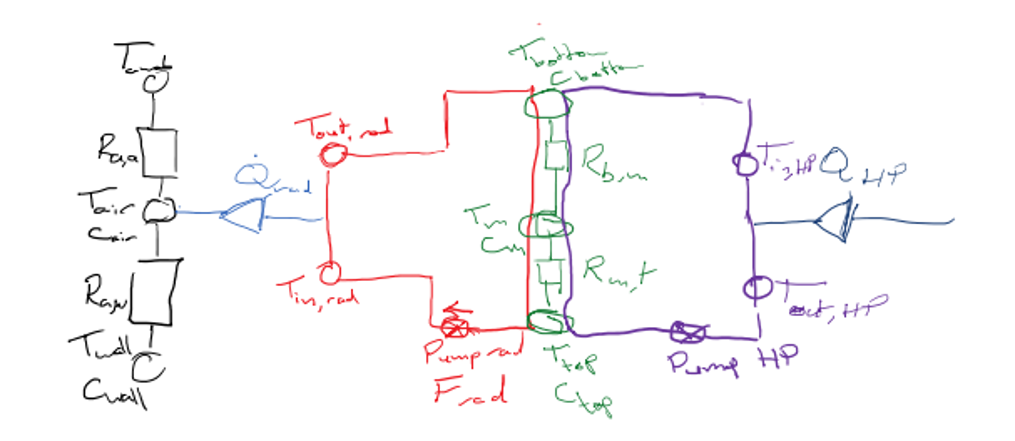
\includegraphics[width=0.9\columnwidth]{Figures/grand_model}
	\caption[Short title]{Grand Model}
	\label{fig:grandmodel}
\end{figure} 

The building itself, in black, generates the differential equations:

\begin{equation}
	\begin{aligned}
		T_{air} \text{:} \quad C_{air}\frac{dT_{air}}{dt} &=\frac{T_{amb}-T_{air}}{R_{air, amb}} + \frac{T_{wall}-T_{air}}{R_{air, wall}} + \dot{Q}_{rad, air} 
		\\ \\
		T_{wall} \text{:} \quad C_{wall}\frac{dT_{wall}}{dt} &=\frac{T_{air}-T_{wall}}{R_{air, wall}}
	\end{aligned}
\end{equation}

$T_{amb}$: given as piecewise constant function, in interval $[t_i, t_{i+1}]$, $T_{amb} = T_{amb, i}$

The radiator element, coupled to the node $T_{air}$, transfers heat to the building at a rate $\dot{Q}_{rad}$. It has a feed temperature $T_{feed}$ and a return temperature $T_{return}$. The radiator is modeled as a "cross-flow" heat exchanger, obeying the "radiator equation":

{\color{blue}
\begin{equation}
	\begin{aligned}
		\dot{Q}_{rad} \text{:} \quad \dot{Q}_{rad} &= C_{rad} \cdot (\Delta T_{LMTD})^n \text{, with } \Delta T_{LMTD} = \frac{T_{feed} - T_{return}}{\ln\left(\frac{T_{feed} -T_{air}}{T_{return} - T_{air}}\right)}
		\\ \\
	    \text{also, :} \quad \dot{Q}_{rad} &= F_{rad} \cdot c_w \cdot (T_{feed} - T_{return})
	\end{aligned}
\end{equation}
}

when $T_{feed}$, $T_{air}$ and $F_{rad}$ are known, we have two equations with two unknowns $\dot{Q}_{rad}$ and $T_{return}$.

{\color{red}Question: when do you solve this system? Do you need to solve this within the time interval $[t_i, t_{i+1}]$?}

Further equations:

\begin{equation}
	\begin{aligned}
        {\color{red}T_{feed}} &= {\color{teal}T_{top}} \\
        {\color{red}T_{return}} & \text{ should follow from equations above.}
    \end{aligned}
\end{equation}

{\color{teal}
\begin{equation}
	\label{eq:buffer}
	\begin{aligned}
	T_{top} \text{:} \quad C_{top}\frac{dT_{top}}{dt} &= \frac{T_{top}-T_{mid}}{-R_{mid, top}} + F_{HP} \cdot c_w \cdot (T_{HP,out} - T_{top}) + \max(F_{rad}-F_{HP}, 0) \cdot c_w \cdot (T_{mid} - T_{top})
    \\ \\
    T_{mid} \text{:} \quad C_{mid}\frac{dT_{mid}}{dt} &= \frac{T_{top}-T_{mid}}{R_{mid, top}} + \frac{T_{mid}-T_{bot}}{-R_{bot, mid}} + \\
    & \max(F_{HP}-F_{rad}, 0) \cdot c_w \cdot (T_{top} - T_{mid}) + \max(F_{rad}-F_{HP}, 0) \cdot c_w \cdot (T_{mid} - T_{bot}) 
    \\ \\
    T_{bot} \text{:} \quad C_{bot}\frac{dT_{bot}}{dt} &= \frac{T_{mid}-T_{bot}}{R_{bot, mid}} + F_{rad} \cdot c_w \cdot (T_{return} - T_{bot}) + \\
    & \max(F_{HP}-F_{rad}, 0) \cdot c_w \cdot (T_{mid} - T_{bot})
	\end{aligned}
\end{equation}
}

\begin{equation}
	\begin{aligned}
		T_{HP,in} &= {\color{teal}T_{bot}} \\
		T_{HP,out} \text{:} \quad \dot{Q}_{HP} &= F_{HP} \cdot c_w \cdot (T_{HP,out} - T_{HP,in}
		\dot{Q}_{HP} &= f(T_{HP,in}\text{,} T_{HP,out}\text{,} T_{src,in}\text{,} T_{src,out}))
	\end{aligned}
\end{equation}

{\color{red} heat pump function? Also here the question is: when to solve this equation?}


Writing out the differential equations in the classical notation:

\begin{equation}
	\begin{aligned}
		C_{air}\frac{dT_{air}}{dt} &= \left[ \frac{-1}{R_{air, amb}} + \frac{-1}{R_{air, wall}} \right]  \cdot T_{air}  + \frac{1}{R_{air, wall}} \cdot T_{wall} + \frac{1}{R_{air, amb}} \cdot T_{amb} + \dot{Q}_{heat, air}
		\\ \\
		C_{wall}\frac{dT_{wall}}{dt} &= \frac{1}{R_{air, wall}} \cdot T_{air} + \frac{-1}{R_{air, wall}}   \cdot T_{wall}
	\end{aligned}
\end{equation}

The differential equations of the 2R-2C house model (in black) be written in matrix notation as:

\begin{subequations}
	\label{eq:matnot}
	\begin{align}
		\mathbf{C} \cdot \boldsymbol{\dot{\theta}} = - \mathbf{K} \cdot \boldsymbol{\theta} + \mathbf{\dot{q}} \\ 
		\mathbf{C} \cdot \boldsymbol{\dot{\theta}} + \mathbf{K} \cdot \boldsymbol{\theta} = \mathbf{\dot{q}}
	\end{align}
\end{subequations}

with:

\begin{equation}
	\mathbf{C} \cdot \boldsymbol{\dot{\theta}} =
	\begin{bmatrix}
		C_{air} & 0 \\
		0 &  C_{wall}
	\end{bmatrix}
	\cdot
	\begin{bmatrix}
		\frac{dT_{air}}{dt} \\
		\frac{dT_{wall}}{dt}
	\end{bmatrix}
\end{equation}

\begin{equation}
	\mathbf{K} \cdot \boldsymbol{\theta} =
	\begin{bmatrix}
		\frac{1}{R_{air, amb}} + \frac{1}{R_{air, wall}} & \frac{-1}{R_{air, wall}} \\
		\frac{-1}{R_{air, wall}} &  \frac{1}{R_{air, wall}}
	\end{bmatrix}
	\cdot
	\begin{bmatrix}
		T_{air} \\
		T_{wall}
	\end{bmatrix}
\end{equation}

\begin{equation}
	\mathbf{\dot{q}} =
	\begin{bmatrix}
		\frac{1}{R_{air, amb}} \cdot T_{amb} + \dot{Q}_{heat, air} \\
		0
	\end{bmatrix}
\end{equation}



The routines in Matlab, Simulink and Python need a \emph{model function} that provides the vector $\boldsymbol{\dot{\theta}}$ for evaluation at any time instance chosen by the algorithm. The equations \eqref{eq:matnot} then should be cast in the following form by left multiplication with $\mathbf{C^{-1}}$.

\begin{subequations}
	\label{eq:matnot_ivp}
	\begin{align}
		\mathbf{C}^{-1} \cdot \mathbf{C} \cdot \boldsymbol{\dot{\theta}} = - \mathbf{C}^{-1} \cdot \mathbf{K} \cdot \boldsymbol{\theta} + \mathbf{C}^{-1} \cdot \mathbf{\dot{q}} \\ 
		\boldsymbol{\dot{\theta}} = - \mathbf{C}^{-1} \cdot \mathbf{K} \cdot \boldsymbol{\theta} + \mathbf{C}^{-1} \cdot \mathbf{\dot{q}}
	\end{align}
\end{subequations}

Since $\mathbf{C}$ is a \emph{diagonal} matrix with positive elements only, its inverse exists and contains the reciprocal elements on its diagonal:

\begin{equation}
	\mathbf{C^{-1}} =
	\begin{bmatrix}
		\frac{1}{C_{air}} & 0 \\
		0 &  \frac{1}{C_{wall}}
	\end{bmatrix}
\end{equation}

This provides the division by the lumped thermal capacitances of the air and wall compartments in the model, necessary for the calculating the derivative vector $\boldsymbol{\dot{\theta}}$ in the model functions. 

Radiator

\begin{equation}
	\begin{aligned}
		C_{feed}\frac{dT_{feed}}{dt} &= F_{rad} \cdot c_w \cdot (T_{top}- T_{feed})
		\\ \\
		C_{return}\frac{dT_{feed}}{dt} &= 
	\end{aligned}
\end{equation} 


\begin{equation}
	\mathbf{C} \cdot \boldsymbol{\dot{\theta}} =
	\begin{bmatrix}
		C_{feed} & 0 \\
		0 &  C_{return}
	\end{bmatrix}
	\cdot
	\begin{bmatrix}
		\frac{dT_{feed}}{dt} \\
		\frac{dT_{return}}{dt}
	\end{bmatrix}
\end{equation}

\begin{equation}
	\mathbf{K} \cdot \boldsymbol{\theta} =
	\begin{bmatrix}
		0 & 0 \\
		0 &  0
	\end{bmatrix}
	\cdot
	\begin{bmatrix}
		T_{feed} \\
		T_{return}
	\end{bmatrix}
\end{equation}

\begin{equation}
	\mathbf{\dot{q}} =
	\begin{bmatrix}
		0 \\
		\dot{Q}_{rad, air}
	\end{bmatrix}
\end{equation}

\subsubsection{Buffer vessel}

The buffer vessel model is the general model for a "stratified (layered) tank". In order to avoid extensive convection in the tank, the model assumes that addition of hot water from the heat source \emph{and} extraction of hot water to the sink (demand) occurs in the \emph{top} layer.  Return flow from the sink is to the \emph{bottom} layer of the vessel.

The differential equations [\ref{eq:buffer}] can be rewritten as:

{\color{teal}
	\begin{equation}
		\begin{aligned}
			C_{top}\frac{dT_{top}}{dt} &= \frac{-1}{R_{mid, top}} (T_{top}-T_{mid}) + \max(F_{rad}-F_{HP}, 0) \cdot (T_{mid} - T_{top}) \\
			&+ F_{HP} \cdot (T_{HP,out} - T_{top})
			\\ \\
			C_{mid}\frac{dT_{mid}}{dt} &= \frac{1}{R_{mid, top}} (T_{top}-T_{mid}) + \frac{-1}{R_{bot, mid}}(T_{mid}-T_{bot}) \\
			& + \max(F_{HP}-F_{rad}, 0) \cdot (T_{top} - T_{mid}) + \max(F_{rad}-F_{HP}, 0)  \cdot (T_{mid} - T_{bot}) 
			\\ \\
			C_{bot}\frac{dT_{bot}}{dt} &= \frac{1}{R_{bot, mid}} (T_{mid}-T_{bot}) + \max(F_{HP} - F_{rad}, 0) \cdot (T_{mid} - T_{bot})\\
			& + F_{rad} \cdot (T_{return} - T_{bot}) 
		\end{aligned}
	\end{equation}
}

These differential equations can be written in matrix notation as previously, but a \emph{convection} matrix $\mathbf{F}$ is added:

\begin{subequations}
	\label{eq:matnot}
	\begin{align}
		\mathbf{C} \cdot \boldsymbol{\dot{\theta}} + \mathbf{K} \cdot \boldsymbol{\theta} + \mathbf{F} \cdot \boldsymbol{\theta}= \mathbf{\dot{q}}
	\end{align}
\end{subequations}

with:

\begin{equation}
	\mathbf{C} \cdot \boldsymbol{\dot{\theta}} =
	\begin{bmatrix}
		C_{top} & 0 & 0 \\
		0 &  C_{mid} & 0 \\
		0 & 0 & C_{bot} \\
	\end{bmatrix}
	\cdot
	\begin{bmatrix}
		\frac{dT_{top}}{dt} \\
		\frac{dT_{mid}}{dt} \\
		\frac{dT_{bot}}{dt}
	\end{bmatrix}
\end{equation}

\begin{equation}
	\mathbf{K} \cdot \boldsymbol{\theta} =
	\begin{bmatrix}
		\frac{1}{R_{mid,top}} & \frac{-1}{R_{mid,top}} & 0\\
		\frac{-1}{R_{mid,top}} &  \frac{1}{R_{mid, top}} + \frac{1}{R_{bot,mid}} & \frac{-1}{R_{bot,mid}}\\
		0 &  \frac{-1}{R_{bot, mid}} & \frac{1}{R_{bot,mid}}
	\end{bmatrix}
	\cdot
	\begin{bmatrix}
		T_{top} \\
		T_{mid} \\
		T_{bot}
	\end{bmatrix}
\end{equation}

\begin{equation}
	\mathbf{F} \cdot \boldsymbol{\theta} =
	\begin{bmatrix}
		F_{HP,out} + F_{rad} & F_{rad} & 0 \\
		F_{rad} &  0  & F_{rad} \\
		0 &  F_{rad} & F_{HP} + F_{rad}
	\end{bmatrix}
	\cdot
	\begin{bmatrix}
		T_{top} \\
		T_{mid} \\
		T_{bot}
	\end{bmatrix}
\end{equation}

\begin{equation}
	\mathbf{\dot{q}} =
	\begin{bmatrix}
		\frac{1}{R_{air, amb}} \cdot T_{amb} + \dot{Q}_{heat, air} \\
		0
	\end{bmatrix}
\end{equation}


F1: [0 1 2 0]

F2: [2 1 0 2]

\begin{equation}
	\mathbf{DF_{F1}} = 
	\begin{bmatrix}
		0 & 1 &-1  \\
	   -1 & 0 & 1  \\
		1 &-1 & 0  \\
	\end{bmatrix}
	\label{eq:DFflow1}
\end{equation}

\begin{equation}
	\mathbf{DF_{F2}} = 
	\begin{bmatrix}
		0 &-1 & 1  \\
	    1 & 0 &-1  \\
	   -1 & 1 & 0  \\
	\end{bmatrix}
	\label{eq:DFflow1}
\end{equation}

In each time step, when the flow sizes have been determined by the control algorithms, each directed-flow-matrix is multiplied by its respected flow size in [$\frac{\text{m}^3}{\text{s}}$]. All resulting matrices can then be added together. Assuming a flow of size $f_1$ and $f_2$ for the flows $F1$ and $F2$, respectively we now get the matrix $\mathbf{SF}$:
\begin{equation}
	\mathbf{SF} = f_1 \cdot \mathbf{DF_{F1}} + f_2 \cdot \mathbf{DF_{F2}} = 
	\begin{bmatrix}
		0     & \dot{f_1}-\dot{f_2} & \dot{f_2}-\dot{f_1} \\
    \dot{ f_2}-\dot{f_1}  & 0       & \dot{f_1}-\dot{f_2} \\
     \dot{f_1}-\dot{f_2}  & \dot{f_2}-\dot{f_1} & 0       
	\end{bmatrix}
	\label{eq:addbufferflows}
\end{equation}

The heat transfer induced by the flows is only in the direction of the water flow. The correct elements are obtained by taking the $\text{min}(\mathbf{SF},0)$, here we mean for each element in $\mathbf{SF}$ we take the minimum of the respective element and 0. Thus, in the case $f_1>f_2$ the matrix $\mathbf{SF}$ will become:
\begin{equation}
	\text{min}(\mathbf{SF},0) =  \begin{bmatrix}
		0     & \dot{f_1}-\dot{f_2} & 0 \\
        0     & 0       & \dot{f_1}-\dot{f_2} \\
     \dot{f_1}-\dot{f_2}  & 0       & 0     
	\end{bmatrix}
	\label{eq:minSFzero}
\end{equation}

Now, the diagonal elements can be computed. The diagonal elements are equal to minus the sum of the off-diagonal elements in its respective row. For the matrix given in equation \ref{eq:minSFzero} this results in the flow matrix $\mathbf{F}$:
\begin{equation}
	\mathbf{F} =  \begin{bmatrix}
		-(\dot{f_1}-\dot{f_2})   & \dot{f_1}-\dot{f_2} & 0 \\
        0     & -(\dot{f_1}-\dot{f_2})       & \dot{f_1}-\dot{f_2} \\
     \dot{f_1}-\dot{f_2}  & 0       & -(\dot{f_1}-\dot{f_2})     
	\end{bmatrix}
	\label{eq:flowmatrix}
\end{equation}

Finally, we need to multiply the resulting flow matrix with the density ($\rho_{w}$) and the specific heat ($c_{w}$), in order to obtain the heat transferred by the water due to the water flows. The resulting matrix can be added to the K matrix as given in equation \ref{eq:CKq_buffer}.

\begin{equation}
	\begin{aligned}
		\dot{f} = v_{pump} \cdot A_{pipe} \qquad & \left[ \frac{m}{s} \cdot m^2 = \frac{m^3}{s}\right] \\
		\dot{f} \cdot \rho_w \cdot c_w \quad \text{has the dimension} \qquad & \left[ \frac{m^3}{s} \cdot m^2 \cdot\frac{kg}{m^3} \cdot \frac{J}{kg \cdot K} = \frac{J}{K \cdot s} = \frac{W}{K}\right]
	\end{aligned}
\end{equation}


\usetikzlibrary{matrix,decorations.pathreplacing}
\pgfkeys{tikz/mymatrixenv/.style={decoration=brace,every left delimiter/.style={xshift=4pt},every right delimiter/.style={xshift=-4pt}}}
\pgfkeys{tikz/mymatrix/.style={matrix of math nodes,left delimiter=[,right delimiter={]},inner sep=1pt,row sep=0em,column sep=0em,nodes={inner sep=6pt}}}

	\begin{tikzpicture}[baseline=0cm,mymatrixenv]
		\matrix [mymatrix,text width=0.6em,align=center] (m)  
		{
			a & b & c \\ 
			d & e & f \\
			g & h & i \\
		};
		\pgfmathsetmacro{\offset}{0.5mm}
		\draw [thick,blue] (m-1-1.west) |- (m-3-3.south) -- cycle;
		\draw [thick,red] (m-1-1.north) -| (m-3-3.east) -- cycle;
		\draw [thick,green,rounded corners=1mm] ([yshift=\offset]m-1-1.west) -- ([xshift=-\offset]m-1-1.north) -- ([yshift=-\offset]m-3-3.east) -- ([xshift=\offset]m-3-3.south) -- cycle;
	\end{tikzpicture}
	
\lstinputlisting[label=lst:stratified, linerange={178-216}, 
caption={StratifiedBufferNew class}] 
{../../housemodel/sourcesink/buffervessels/stratified.py}



\subsubsection{Radiator}

In a radiator, the heat transport is in good approximation only due to \emph{convection} of a gas (steam) or liquid (water, glycol, brine) For a liquid, the following points of view may be taken:
The equations for the radiator element are:

{\color{blue}
	\begin{equation}
		\label{eq:radnonlin}
		\begin{aligned}
			F_{rad} &= \dot{f} \cdot \rho \cdot c_w  \\
			F_{rad} &= \dot{m} \cdot c_w  
		\end{aligned}
	\end{equation}
}
where: \\
$\rho$ is the density of the liquid in $[kg/m^3]$ \\
$c_w$ is the specific heat capacity of water: $4.2 \cdot 10^3 J/(kg \cdot K)$ \\
$\dot{f}$ is the liquid volume flow in $[m^3/s]$ \\
$\dot{m}$ is the liquid mass flow in $[kg/s]$ \\

The equations for the heat transfer of the radiator are: 

{\color{blue}
	\begin{equation}
		\label{eq:radnonlin}
		\begin{aligned}
			\dot{Q}_{rad} &- C_{rad} \cdot (\Delta T_{LMTD})^n &= 0 \\
			\dot{Q}_{rad} &- F_{rad} \cdot (T_{feed} - T_{return}) &= 0 \\ \\
			&\text{with } \Delta T_{LMTD} = \frac{T_{feed} - T_{return}}{\ln\left(\frac{T_{feed} -T_{air}}{T_{return} - T_{air}}\right)}
		\end{aligned}
	\end{equation}
}

This nonlinear system of equations can be solved for the two unknowns $[\dot{Q}_{rad} \quad T_{return}]$, if input data $T_{feed}$, $ T_{amb}$, $C_{rad}$ and $F_{rad}$ are provided. A solver needs the function template in Eq.~\ref{eq:radnonlin}, with the unknowns vector as input variable. Furthermore, the Jacobian of the function template has to be calculated. Evaluation of an analytical expression of the partial derivatives in the Jacobian always outperforms numerical derivative calculations. Thus, for the upper equation (function) in set \ref{eq:radnonlin}:

\begin{equation}
	\begin{aligned}
		\begin{matrix}
			\frac{\partial f}{\partial \dot{Q}_{rad}} &= 1 \\ 
			\\
			\dfrac{\partial f}{\partial T_{return}} &= -Cn\cdot \dfrac{\left(\frac{T_1-T_2}{\ln\left(\frac{T_1-T_3}{T_2-T_3}\right)}\right)^{n-1}\,\left(\frac{T_1-T_2}{T_2-T_3}-\ln\left(\frac{T_1-T_3}{T_2-T_3}\right)\right)}{\ln^2\left(\frac{T_1-T_3}{T_2-T_3}\right)} \\ \\
		\end{matrix}
	\end{aligned}
\end{equation} 
for the second equation:
\begin{equation}
	\begin{aligned}
		\begin{matrix}
			\frac{\partial f}{\partial \dot{Q}_{rad}} &= 1 \\ \\
			\frac{\partial f}{\partial T_{return}} &= -F_{rad}
		\end{matrix}
	\end{aligned}
\end{equation} 

See: \url{https://www.derivative-calculator.net/}.

The Jacobian matrix 
$$\mathbf{J}_{i,j}=\dfrac{\partial f_{i}(\mathbf{x})}{\partial x_{j}}$$
becomes:
\begin{equation}
	\begin{aligned}
		\begin{bmatrix}
			\dfrac{\partial f_1}{\partial \dot{Q}_{rad}} & \dfrac{\partial f_1}{\partial T_{return}} \\ 
			\vspace{2pt} \\
			\dfrac{\partial f_2}{\partial \dot{Q}_{rad}} & \dfrac{\partial f_2}{\partial T_{return}}
		\end{bmatrix}
	\end{aligned}
\end{equation} 

with:

\begin{equation}
	\begin{aligned}
		\mathbf{x} =
		\begin{bmatrix}
			\dot{Q}_{rad} \\ 
			T_{return}
		\end{bmatrix}
	\end{aligned}
\end{equation}

The properties and the calculation of $\mathbf{x}$ is implemented in Python in the \textsf{Radiator} class.
The methods of this class are:
\begin{itemize}
	\item \textsf{\_\_init\_\_}: initializes the class members. Members starting with \_\_* are private members.
	\item \textsf{get\_lmtd}: returns the value of private member \_\_lmtd.
	\item \textsf{func\_rad}: calculates radiator equations and partial derivatives.
	\item \textsf{update}: uses \textsf{scipy.optimize.root()} to find the roots $\mathbf{x}$ of the radiator equations.
\end{itemize}

\lstinputlisting[label=lst:Radiator, linerange={78-109}, 
caption={Radiator class}] 
{../../housemodel/sourcesink/radiators/radiators.py}

The Radiator class uses a helper function \textsf{LMTD\_radiator} to determine the effective temperature drop:

\lstinputlisting[label=lst:lmtd, linerange={16-46}, 
caption={LMTD\_radiator function}] 
{../../housemodel/sourcesink/radiators/radiators.py}

Other radiator models can be found in \cite{TolRadiator, TolThesis}.

The Radiator object has the following attributes:

\begin{itemize}
	\item a "hot" node $T_{feed}$. This is a node of type \textsf{CapacityNode} (see section \ref{sec:capnode}).
	\item a "cold" node $T_{return}$. This is a node of type \textsf{FixedNode} (see section \ref{sec:fixnode}), with a variable temperature, but no heat capacity.
	\item an "effective" temperature \emph{difference} with the surroundings of the radiator \textit{i.e.} the interior of the building in the model.
	\item the instantaneous thermal power delivered by the radiator to the interior of the building.
	\item a \textsf{Flow} object (shared with \textit{e.g.} a buffer vessel).
\end{itemize} 

\subsection{Model component properties towards an integrated implementation}
Here we summarize the properties of the different model components. 

\subsubsection{Capacity Node} \label{sec:capnode}

\textbf{description}: A capacity node represents the heat capacity of a part of the system, \textit{for example}, the air in a room, or the water in a layer of the buffer vessel. Within the model, for each capacity node the evolution of the temperature over time will be computed. The capacity nodes are used in the components of the house model and the buffer vessel. 
\\
\textbf{properties}

\begin{itemize}
	\item \emph{label}: unique `name' for the node. This should be provided in the \textbf{input}.
	\item \emph{tag}: index of the node in the resulting model. Translates to row-index in the matrices and $\mathbf{\dot{q}}$-vector.
	\item \emph{heat\_capacity}: the heat capacity [J/K]. This is constant over time and should be provided in the \textbf{input}. Capacity should be greater than zero and finite.  
	\item \emph{temperature}: the temperature [K]. This will be computed by the model. For each node the model should be able to output a temperature profile over the duration of the simulation
\end{itemize}

In the listing below, from the module \texttt{components.py}, the definition of the component as a \texttt{dataclass} is shown: 
\begin{minipage}{\linewidth}
\lstinputlisting[label=lst:capnode, linerange={4-9}, 
caption={Capacity Node}]
{../../housemodel/basics/components.py}
\end{minipage}

\subsubsection{Fixed temperature Node (external node)} \label{sec:fixnode}
\textbf{description}: This is a node with a predefined temperature. This temperature will not change due to heat exchange with its surrounding nodes. The predefined (external) temperature should be constant within a given time interval. This node represents a part of the system with a very large heat capacity (much larger than other components), \textit{for example}, the ambient air or the ground. 

\textbf{properties}
\begin{itemize}
	\item \emph{label}: unique 'name' for identification. This should be provided in the \textbf{input}.
	\item \emph{connection(s)} to other model nodes: every fixed temperature node is connected to at least one capacity node, via a heat conductance edge. This edge, and its corresponding heat conductance, "belongs" to the fixed temperature node.
	\item contribution to \textbf{K}-matrix: based on the (time-dependent) temperature and the conductances, the diagonal element in the \textbf{K}-matrix corresponding to the connected capacity nodes should be updated.
	\item \emph{temperature} [K] or [\degree C]: for every given time the temperature of this node should be defined. For this a temperature profile should be provided in the \textbf{input}. The temperature profile can be a list of tuples of the form [start\_time , temperature]. At every time interval for which the model is evaluated the corresponding temperature of the node should be obtained. For this a function \texttt{set\_node\_temperature} is needed. 
	\item contribution to \textbf{q}-vector: based on the (time-dependent) temperature and the conductances, the element in the \textbf{q}-vector corresponding capacity nodes should be updated. This is update may be done in the same function as the update for the \textbf{K}-matrix. The update value is the same for both terms, except for the sign. 
\end{itemize}
\emph{NOTE}: The temperature of the node should remain constant over the entire interval of model solving, so moments of switching temperature should coincide with the start and end of these intervals. This may be enforced by limiting the options for 'start\_time' (for example only multiples of 10 minutes). An alternative could be that the profile is always defined based on the times as given by the NEN5060. The NEN5060 will, most likely, provide the profile of the ambient air temperature. When we would require all profiles of the same shape and size the reading and processing can be done in the same fashion for all nodes. 

In the listing below, from the module \texttt{components.py}, the definition of the component as a \texttt{dataclass} is shown:
\begin{minipage}{\linewidth}
\lstinputlisting[label=lst:fixnode, linerange={12-20}, 
caption={Fixed Node (external node)}] 
{../../housemodel/basics/components.py}
\end{minipage}

The attribute \texttt{connected\_to} is a list with elements \texttt{[tag, conductivity]}. This attribute contains all information for building the \textbf{k}-matrix. In most cases the attribute \texttt{connected\_to} does not change during a simulation. Only the attribute \texttt{temp} is updated at regular intervals (see method \texttt{update}). The contribution to the $\mathbf{\dot{q}}$-vector then has to be updated as well.

\subsubsection{Heat conductance Edges}
\textbf{description}: A heat conductance edge represents the possibility to exchange heat between the two connected nodes (either capacity node or temperature node). Heat will be transferred from the node with high temperature to the node with low temperature. For example, an edge between the nodes 'air' and 'walls' indicates that heat can be transferred from the air to the wall, and the other way around.  

\textbf{properties}
\begin{itemize}
	\item \emph{label}: name of the edge. This should be provided in the \textbf{input}.
	\item \emph{connected\_nodes}: a pair of connected nodes. Each edge connects two nodes. This should be provided in the \textbf{input}. 
	\item \emph{conductance\_value} [J/K] or [J/\degree C]. This should be provided in the \textbf{input}.
\end{itemize}

\lstinputlisting[label=lst:capnode, linerange={23-29}, 
caption={Conductance Edges}] 
{../../housemodel/basics/components.py}

\subsubsection{Fluid Flow}
\emph{NOTE}: the definition of the fluid flows in this section has its limitations. Only basic closed loops without splits in the 'pipes' can be modeled. This is fine as a starting point. However, when more complex scenarios with complex fluid flows are required a more generic formalism is needed for the modeling of the fluid flows. In this case, a system with flow edges and flow nodes may be a possible solution. The open challenges here are: 1. how to define the flow network (next to / in combination with the heat conductance network),  2. how to compute the flow rates in the more complex system. 

\textbf{description:} A fluid flow represents a \emph{closed} loop over a set of nodes (with or without heat capacity). The flow rate is the same for all nodes and edges within the loop. The flow rate may change over time, but is assumed to be constant within a given time interval, and changes are assumed to be instantaneous. Thus, the flow rate can be described by a step-function. This flow rate should be controlled, either in a on/off manner, or in m (???)

\textbf{properties}
\begin{itemize}
	\item \emph{label}: name of the fluid flow. This should be provided in the \textbf{input}.
	\item \emph{flow\_rate}: The flow rate of the fluid in $\text{m}^3/\text{s}$ (or another unit that fits). This flow rate may change over time, matrices related to the heat transfer induced by the fluid flow need to be updated accordingly, see Section \ref{s:flow_matrices}. 
	\item \emph{density}: density of the fluid in [$\frac{kg}{m^3}$]. One fixed density will be used (no temperature dependence is taken into account here). This should be provided in the \textbf{input}.
	\item \emph{heat\_capacity}: heat capacity of the fluid in [$\frac{J}{kg \cdot K}$]. This should be provided in the \textbf{input}.
	\item \emph{connected\_nodes}: An \emph{ordered} list of the nodes through which the fluid flow runs, the order is determined by the direction the fluid will be pumped through the network. Start and end of the list need to be the same node. This ensures the required closed loop. This should be provided in the \textbf{input}. From this ordered list a "directed-flow-matrix" can be set-up as indicated in Section \ref{s:flow_matrices}. 
\end{itemize}

\lstinputlisting[label=lst:flows, linerange={8-16}, 
caption={Flow}] 
{../../housemodel/basics/flows.py}

\subsubsection{flow network}
\textbf{description}: multiple fluid flows can be combined in a flow network. The current  methodology is limited to two flows (specifically, two flows that both are connected to a buffer vessel). 

\textbf{properties}
\begin{itemize}
	\item \emph{sum\_flows}: based on the directed flow matrices and the flow rates, a total matrix can be created (cf. Section \ref{s:flow_matrices})
	\item \emph{heat\_transfer\_matrix}: from the sum\_flow matrix, and the fluid density and heat capacity the corresponding heat transfer matrix can be created.  
\end{itemize}
%
%
%\subsubsection{flow edges}
%\emph{NOTE}:This and the following parts on flows are a first step to a more general flow network design. Flows have been defined earlier based on a ordered list which gives all edges directly. The flows we have envisioned so far are based on closed loops. The loops may be interconnected with each other, creating a network of flows. Each loop should contain a pump that drives the flow. A flow edge connects \textbf{two} flow nodes. Within the edge no heat loss is taken into account. A split of the flow should be modeled by adding a node with more than two connected flow edges. 
%
%\textbf{description} A flow edge represents the possibility of heat transfer between capacities by the flow of a medium. In contrast to a heat conductance edge the transfer is uni-directional, in the direction of the flow. 
%\textbf{properties}
%\begin{itemize}	
	%\item node\_in: node from which the flow comes. 
	%\item node\_out: node to which the flow goes. 	
	%\item flow\_rate: this is variable and should be controlled somehow. The flow rate in a edge depends on the incoming flow (what comes in should go out) 
%\end{itemize}
%
%\lstinputlisting[label=lst:capnode, linerange={35-41}, 
%caption={Flow Edges}] 
%{../../housemodel/buildings/components.py}
%
%\subsubsection{flow node}
%\begin{itemize}
	%\item nr\_connections: should be greater or equal 2. Each connection may be either incoming or outgoing, depending on the pump rates that drive the flows through the connected edges. As the pump rates may change the solution to the flow rate through each flow connection may change as well. Solving this for an arbitrary network will need further research. (The procedure might be very similar as solving for currents in an electrical network using Kirchhoff's circuit laws, possibly interesting material can also be found in the field of "\textit{pipe network analysis}". The pipe networks in the model should remain relatively basic. It is possibly taking it to far, making the modeling concept so generic that it will solve arbitrary flow networks. However, alternatively some check is needed whether the system is set-up as expected. 
	%\item flow division ratio: When multiple outgoing connections are available one can potentially add the concept of controlling the division of the outgoing flows by some valve. Adding this feature to the model would make it even more complex. A network solving method would be needed to incorporate this. 
	%\item heat\_capacity: unlike the edges, a flow node can have a heat capacity (like a capacity node). It does not need to have it when it would be used as a pipe junction. In this case the capacity will be zero. Nodes with a positive heat capacity can also be connected in a heat conductance network. 
	%\item temperature: temperature of the medium in the node (only needed when the node has a positive capacity)
%\end{itemize}
%
%\subsubsection{flow pump node}
%\textbf{description}: A flow pump is a node in the flow 'network' which determines the flow rate of the fluid going through the flow-network, both upstream and down stream of the pump. 
%
%\textbf{properties}
%\begin{itemize}
	%\item flow\_rate
	%\item incoming\_connection: in order to be able to define a flow direction the notion of the incoming link and outgoing link is needed. 
	%\item outgoing\_connection
%\end{itemize}  
%

\subsubsection{house module}
\textbf{description}: The house module is an abstraction of the main heat capacities of a house, and the heat conductances within. \emph{NOTE}, capacities can be connected to other model modules by means of heat conductance edges or possibly flow edges. There is potentially much freedom in the model design here. Question to be solved here is how do we define the inter-connectivity in the input? Which module is 'leading' in making the connection. My (Marijn) first idea is to let the house module be 'passive' here, that is, connections to the house module are part of the connecting-module.    

\textbf{properties}
\begin{itemize}
	\item list\_capacity\_nodes. input from (excel) table.
	\item lis\_heat\_conductance\_edges. input from (excel) table.
	\item C\_matrix: based on capacities a house C-matrix can be composed. (diagonal matrix)
	\item k\_matrix: based on the edges a house k\_matrix can be composed. (method based on graph theory functions)
\end{itemize}


\subsubsection{fixed temperatures module}
\textbf{description} The fixed temperatures module is a collection of all fixed temperature nodes that are connected to the different other parts of the running model. For each node the temperature profile over time is checked, and the temperature is updated accordingly. 

\textbf{properties}
\begin{itemize}
	\item list\_fixed\_temperature\_nodes
	\item updating\_function: function that loops over all fixed nodes, and makes sure every node is up to date with respect to the temperature at the given time. The updated contributions to \textbf{k}-matrix and \textbf{q}-vector should be added and passed to the model solver. 
\end{itemize}


\subsection{buffer module}
\textbf{description}: The buffer module is an abstract representation of a heat buffer vessel. The vessel is build up of a set of $n$ layers. Each layer has a heat conductance edge to the layer directly above and below. Also, a conductance edge to the surrounding air is possible, represented by a fixed temperature node (this works similar as for a house). An alternative is that the surrounding air is a capacity node, which can be part of, or connected to the house module. This last scenario is more complex to incorporate in the model, as this connection is not part of either module (buffer or house), but is a 'special' inter-module connection. Next to the heat conductance edges, the buffer also has flow connections. Internally, flow connections exist between adjacent layers, these are bi-directional (the flow can go both directions, but at every moment in time the flow only one direction is active). Also flow connections, coming in and flowing out of both the top and bottom layer are possible. 

\textbf{properties}
\begin{itemize}
	\item nr\_layers
	\item node\_list: the buffer consists of multiple flow nodes with capacity. The nodes corresponding to the top and bottom layer will have flow connections. 
	\item internal\_conductance\_edges: an internal conductance network defines the internal heat-exchange. With this set of internal edges the a  \textbf{k}-matrix  for the buffer can be build. This should be incorporated in the overall model \textbf{k}
	\item 
\end{itemize}

\subsection{Heat Pump}

A heat pump can be modeled in several ways. A straightforward approach is to reduce the heat pump to two fixed nodes, external to the building system. These nodes represent the evaporator and condensor \emph{exit} temperatures $T_{evap}$ and $T_{cond}$. In case of a air-water heatpump, $T_{evap}$ can be approched with the instantaneous outdoor (ambient) temperature from the weather conditions. For a heat pump with a liquid heat source this will be the source temperature, in any cases a ground source. $T_{cond}$ can be derived from a heating curve ($T_{cond}$ vs. $T_{outdoor}$) or from a heat pump functional model.

\textbf{properties}
\begin{itemize}
	\item $T_{evap}$.
	\item $T_{cond}$. 
	\item COP
	\item Thermal power
\end{itemize}

The heat pump will deliver its thermal power via an internal heat exchanger from the refrigerant to a liquid heat carrier (water) in a buffer vessel. There are a few options for the connection of the buffer vessel:

\subsubsection{4-way connection}

The most straightforward connection method is a 4-way connection, as shown in Figure~\ref{fig:4way}. The heat source (heat pump) thermally loads the buffer vessel in the top layer. The thermal demand is also taken from the top layer. For low-temperature radiators or a floor heating circuit there is a mixing valve that short circuits feed and return water, to provide an adjustable temperature heat source for the delivery system. The remaining return flow from the delivery system is passed back to the bottom layer of the buffer vessel. The heat source return water is also taken from the bottom layer.

\begin{figure}[H]
	\centering
	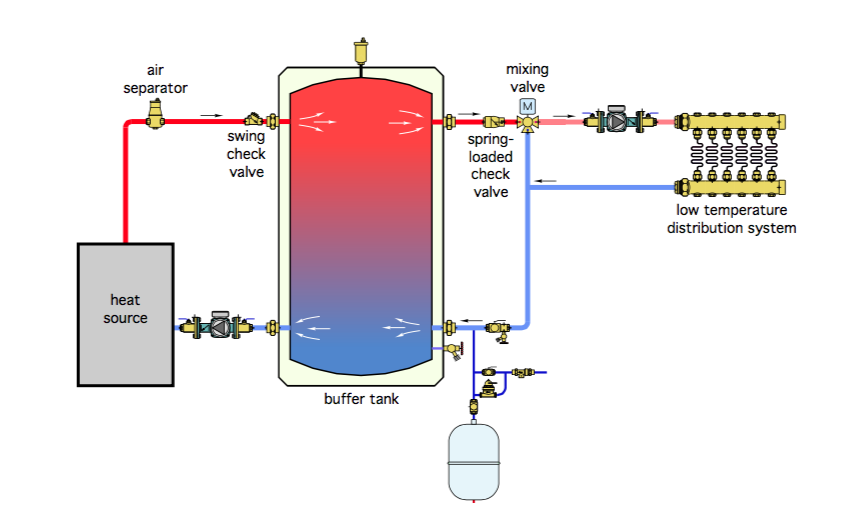
\includegraphics[width=0.7\columnwidth]{Figures/4-way buffer connection}
	\caption[Short title]{4-way connection of stratified buffer vessel.}
	\label{fig:4way}
\end{figure} 

\begin{figure}[H]
	\centering
	\begin{subfigure}[b]{0.45\textwidth}
		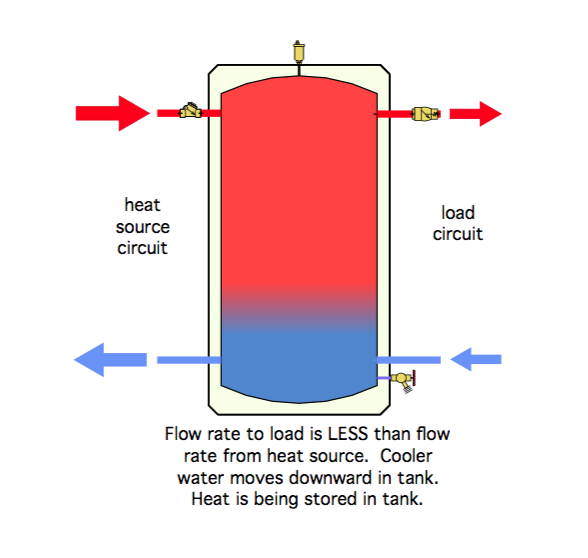
\includegraphics[width=\textwidth]{Figures/4-way buffer loaded}
		\caption{Buffer vessel loading...}
		\label{fig:4way_loaded}
	\end{subfigure}
	\hfill
	\begin{subfigure}[b]{0.45\textwidth}
		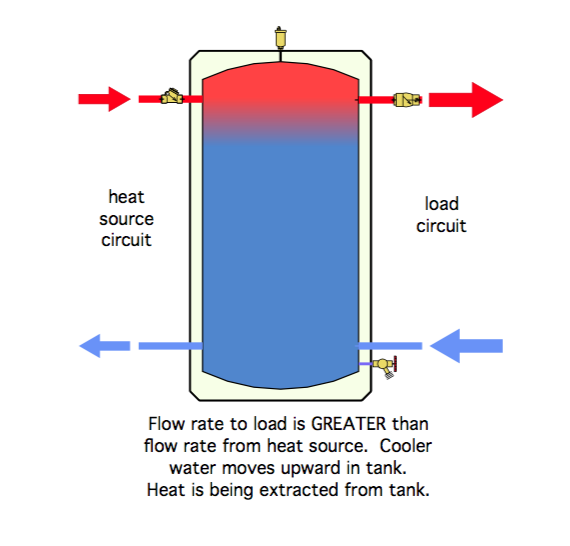
\includegraphics[width=\textwidth]{Figures/4-way buffer unloading}
		\caption{Buffer vessel unloading...}
		\label{fig:4way_unloading}
	\end{subfigure}
	\caption{Stratified buffer vessel dynamics.}
	\label{fig:4way_dynamics}
\end{figure}

\subsubsection{2-way connection}

\begin{figure}[H]
	\centering
	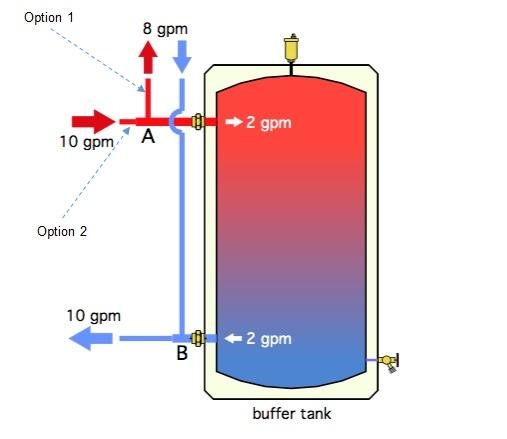
\includegraphics[width=0.5\columnwidth]{Figures/2-way buffer connection}
	\caption[Short title]{2-way connection of stratified buffer vessel.}
	\label{fig:2way}
\end{figure} 

\subsection{Scripts}

\subsubsection{Use Case}

\begin{itemize}
	\item \textbf{import classes}
\end{itemize}

\begin{itemize}
	\item \textbf{instantiate classes}
\end{itemize}

\begin{itemize}
	\item \textbf{set up matrices}
\end{itemize}

\begin{itemize}
	\item \textbf{perform calculations}
\end{itemize}

Simulations can be run as a Python script or as an IPython (Jupyter) notebook. The structure of a script can be summarized as follows:

\begin{itemize}
	\item read configuration file. This file is written in \textsf{*.yaml} format. The parameters in the file are converted to a variable (suggested name: \texttt{param}) of type \texttt{dict}.
	\item create an instance of the \texttt{Building} class. Example: \texttt{h = Building("MyHouse")}.
	
	\lstinputlisting[label=lst:house, linerange={19-39}, 
	caption={The Building class}] 
	{../../housemodel/buildings/building.py}
	
	\item read the nodes of the Building model with the method \texttt{nodes\_from\_dict(param["Building"]["nodes"])}
	\item fill the inverse of the capacity matrix $\mathbf{C^{-1}}$ using the method \texttt{fill\_c\_inv}().
	\item read \emph{all} fixed nodes using the method \texttt{boundaries\_from\_dict(param["boundaries"])}. \\ The method copies the "outdoor" external node to the \texttt{Building.ambient} node.
	\item initialize the $\mathbf{K}$-matrix and add the conductivity between the building nodes and ambient to the diagonal elements using the method \texttt{make\_k\_ext\_and\_add\_ambient()}.
	\item at this point we can read \emph{all} edges in the model using the method \texttt{edges\_from\_dict(param["edges"])} and add the non-diagonal elements to $\mathbf{K}$ with the method \texttt{fill\_k(param["edges"])}. However, this can only be done for the thermal conductivities \emph{within} the Building subsystem. Thermal conductivities \emph{between} subsystems (\textit{e.g.} between the Building contents and a Radiator) have to be added after assembly of the subsystems (matrices) into a complete model (set of differential equations). Therefore, the $\mathbf{K}$-matrix is completed \emph{after} merging the matrices of the subsystems. 
\end{itemize}

	\begin{equation}
		\mathbf{K} \cdot \boldsymbol{\theta} =
		\left[~
		\underbrace{
		\begin{bmatrix}
			\frac{1}{R_{air, wall}} & \frac{-1}{R_{air, wall}} \\
			\frac{-1}{R_{air, wall}} &  \frac{1}{R_{air, wall}}
		\end{bmatrix}
	    }_{\mathbf{K}_{int}}
	    +
	    \underbrace{
	    \begin{bmatrix}
	    	\frac{1}{R_{air, amb}} & 0 \\
	    	0 &  0
	    \end{bmatrix}
        }_{\mathbf{K}_{ext}}
        ~\right]
		\cdot
		\begin{bmatrix}
			T_{air} \\
			T_{wall}
		\end{bmatrix}
	\end{equation}
\\
\begin{itemize}
	\item Similarly, a buffer vessel can be created with \texttt{b = StratifiedBuffer("Buffervessel")}.
	\item run \texttt{b.nodes\_from\_dict(param["Buffer"]["nodes"])} and \texttt{b.fill\_c\_inv()} to create the inverse capacity matrix $\mathbf{C^{-1}}$ for the buffer vessel. The nodes are equivalent to the layers of a stratified buffer tank.
	\item The buffer vessel has a "ambient" temperature which is an "indoor" temperature for an attic or basement room. This temperature can be taken as a constant for the complete simulation period. Apply the functions \texttt{b.boundaries\_from\_dict(param["boundaries"])} (selects "indoor" as ambient) and 
	\texttt{b.add\_ambient\_to\_k()}.
\end{itemize}

\begin{equation}
	\mathbf{K} \cdot \boldsymbol{\theta} =
	\left[~
    \underbrace{
	\begin{bmatrix}
		\frac{1}{R_{top, mid}}  & \frac{-1}{R_{top, mid}} & 0\\
		\frac{-1}{R_{top, mid}} &  \frac{1}{R_{top, mid}} + \frac{1}{R_{mid, bot}} & \frac{-1}{R_{mid, bot}}\\
		0  &  \frac{-1}{R_{mid, bot}} & \frac{1}{R_{mid, bot}}
	\end{bmatrix}
	}_{\mathbf{K}_{int}}
	+
	\underbrace{
	\begin{bmatrix}
		\frac{1}{R_{top, amb}} & 0 & 0 \\
	    0 & \frac{1}{R_{mid, amb}} & 0  \\
	    0 & 0 & \frac{1}{R_{bot, amb}} 
	\end{bmatrix}
    }_{\mathbf{K}_{ext}}
	~\right]
	\cdot
	\begin{bmatrix}
		T_{top} \\
		T_{mid}  \\
		T_{bot} 
	\end{bmatrix}
\end{equation}
\\

\begin{itemize}
	\item  A very simple radiator model consists of a CapacityNode, coupled to the contents ("air") of the Building subsystem. This can be implemented by calling \texttt{r = LinearRadiator("SimpleRadiator")}, \\
	\texttt{r.nodes\_from\_dict(param["Radiator"]["nodes"])} and \texttt{r.fill\_c\_inv()}. $\mathbf{C^{-1}}$ is a matrix of rank 1 in this case (numpy.ndarray(1,1)), and not a scalar.
	\item the LinearRadiator object does not have an "ambient" fixed (external) node contributing to the $\mathbf{K}$-matrix.
\end{itemize}

	\begin{equation}
	\mathbf{K} \cdot \boldsymbol{\theta} =
	\left[~
	\underbrace{
		\begin{bmatrix}
			\frac{1}{R_{air, rad}} 
		\end{bmatrix}
	}_{\mathbf{K}_{int}}
	+
	\underbrace{
		\begin{bmatrix}
			0
		\end{bmatrix}
	}_{\mathbf{K}_{ext}}
	~\right]
	\cdot
	\begin{bmatrix}
		T_{rad}
	\end{bmatrix}
\end{equation}
\\
\begin{itemize}
	\item a complete model can be assembled from the partial models. it is created with \\ \texttt{total = TotalSystem("HouseWithRadiator", [r, h])}. The list \texttt{[r, h]} of partial models is then sorted with     \texttt{total.sort\_parts()} so that the previously assigned tags correspond to the rows of the total system matrices.
	\item compose the $\mathbf{C^{-1}}$-matrix from the parts with \texttt{total.merge\_c\_inv()}.
	\item merge the tag\_lists with \texttt{total.merge\_tag\_lists()}. TotalSystem.tag\_list should be ordered.
	
	\item compose the $\mathbf{K}$-matrix from the parts with \texttt{total.edges\_from\_dict(param["edges"])} and \\ \texttt{total.fill\_k(param["edges"])}.
	\item compose the $\mathbf{K_{ext}}$-matrix from the parts with \texttt{total.merge\_k\_ext()}.
	\item add $\mathbf{K}$ and $\mathbf{K_{ext}}$ with \texttt{total.k\_mat += total.k\_ext\_mat}.
	
	\item create an empty $\mathbf{\dot{q}}$-vector with \texttt{TotalSystem.make\_empty\_q\_vec()}.
\end{itemize}

\begin{footnotesize}
	
\textbf{Note:} generation of the $\mathbf{K_{int}}$-matrix of the total system there are a number of feasible approaches:

\begin{enumerate}
	\item  read \emph{all} edges in the model using the methods \texttt{TotalSystem.edges\_from\_dict(param["edges"])} and \\ \texttt{TotalSystem.fill\_k(param["edges"])}.
	This can only be done in one step, after the parts (\texttt{Building} etc.) in the TotalSystem have been defined. The assumption is that the edge list for the total system \textit{i.e.} all edges \emph{within} parts and \emph{between} parts can be read from the section "edges" in the configuration file. If parts of the TotalSystem e.g. the StratifiedBuffer class generate their own internal thermal conductance edges, these edges have to be backconverted (serialized) into a *.yaml string before merging with the other edges. Alternatively, an intermediary version of the configuration file has to be generated before \texttt{TotalSystem.edges\_from\_dict(param["edges"])} can be called. This results in a somewhat awkward script, looking differently depending on the presence of a buffer vessel in the total system.
	
	\item read the edges \emph{within} a subsystem (part) from its own section in the configuration file. This works well for parts that do not generate their own edges and edge list. Parts derived from e.g. the StratifiedBuffer class generate their own edges and edge list, which is not spelled out in the configuration file. The top-level "edges" section in the configuration file only contains the edges \emph{between} parts of the TotalSystem. This approach enables merging of edges from the configuration file with edges self-generated from physical parameters by some subsystem classes.
	
	with the latter approach, two strategies for generating the total $\mathbf{K_{int}}$-matrix can be followed:

	\begin{enumerate}
		\item merge the edge lists (read and generated) from all parts of the total system with the edge list containing the edges between the parts. This requires merging  the edge lists into a flattened \texttt{TotalSystem.edge\_list}.  A $\mathbf{K_{int}}$-matrix for the total system can be generated with the method \texttt{fill\_k(TotalSystem.edge\_list)}. 
		\item Alternatively, a block diagonal $\mathbf{K_{int}}$-matrix can be constructed from $\mathbf{K_{int}}$-matrices calculated for  each part. Then the edges between the parts have to be added one by one with a dedicated method of the TotalSystem class. Thermal conductivities \emph{between} subsystems (\textit{e.g.} between the Building contents and a Radiator) are thus added after assembly of the subsystems (matrices) into a complete model (set of differential equations). The $\mathbf{K}$-matrix is completed \emph{after} merging the matrices of the subsystems. 
	\end{enumerate} 
\end{enumerate}
    
    After testing out these different approaches, strategy 2(a) is chosen.  

\end{footnotesize}

\newpage

\section{Solar irradiation and PV yield}

In the house model, energy supply from solar irradition plays an important role. Firstly, solar energy enters the building through windows and poorly isolated surfaces. In winter, this reduces the cost of heating the building. in summer, however, this leads to an extra energy expenditure for cooling the building, which may attain uncomfortable indoor temperature levels in case of large window surfaces or poor isolation.

A second issue is that the yield of PV and PVT panels, which are often installed nowadays, depends on the solar irradiation. Weather conditions, especially the cloud cover density have a strong influence on the electric power and energy yield of these installations.

Therefore, it is important to be able to calculate the solar irradiation quantity, spectral distribution and spatial properties. Only then, a reliable estimation of the energy demand, and of the useful fraction of solar irradiation can be made.

\subsection{Solar software}

Software for calculation of solar irradiation on the surface of the earth exists in many shapes and implementations. To achieve the final goal, calculation of the solar (power) falling on a surface with a certain orientation, a number of steps have to be carried out.

\begin{enumerate}
	\item establish the geolocation of the object (building, PV(T) panel) of interest
	\item establish the time instant or time range of interest
	\item convert the time instant to local, timezone-aware time or UTC
	\item find the apparent position of the sun in the sky (azimuth and inclination)
	\item determine the attenuation of the earth's atmosphere for the geolocation and time(s) of interest
	\item determine the DNI 
	\item determine the orientation of the surface of interest (azimuth and inclination)
	\item determine the direct, diffuse and global irradiation on the surface
	\item determine the fraction of the solar irradiation that is effective as an energy source (window transmittance, PV(T) efficiency)
\end{enumerate}

Among the packages available for solar irradiation calculations, we find:

\begin{itemize}
	\item \textsf{PV\_LIB Toolbox}: available for Matlab and Python \cite{PV_LIB_main, PV_LIB_Python, PV_LIB_ReadTheDocs, PV_LIB_GitHub}.
	\item \textsf{solarenergy}: available as Python package \cite{SolarEnergy_ReadTheDocs, SolarEnergy_GitHub}
	\item \textsf{qsun}: available as Matlab function or Python function.
\end{itemize}

\subsection{Geolocation}

The location of a building or installation needs to be given in \emph{latitude} and \emph{longitude}, in units of degrees with a decimal point. Division in arcminutes and arcseconds is less common nowadays, since the introduction of GPS. Latitude is positive for the northern hemisphere, negative to the south of the equator. The equator itself is zero latitude. Longitude is positive to the east of the Royal Observatory in Greenwich, London, UK, negative to the west of London. The Meridian of Greenwich runs from the North pole to the South Pole through London and has zero longitude. At the poles, latitude is $\pm 90$ degrees and longitude is undefined.

For \textbf{Arnhem}, NL, a \textbf{latitude of 52.0 degrees} and a \textbf{longitude of 6.0 degrees} may be used as an approximation to the geolocation. In reality this geolocation is found in a field between Velp and Rheden, NL.

\begin{itemize}
	\item \textsf{PV\_LIB Toolbox} has a  module \textsf{location.py}. In this module, a class \textsf{Location} is defined, with attributes  \emph{latitude} and \emph{longitude}. These attributes are in \emph{decimal degrees} \textit{i.e.} 52.0 and 6.0. 
	\item \textsf{solarenergy} has a module \textsf{radiation.py} with  a function \textsf{sun\_position\_from\_date\_and\_time}. Input parameters to this function are \emph{longitude} and \emph{latitude} in \emph{radians}. The \textsf{solarenergy} has a conversion constant \textsf{d2r} to convert from decimal degrees to radians. 
	\item \textsf{qsun}: longitude and latitude are not input parameters. They are fixed: the chosen location is for De Bilt, NL (52.1 N, 5.1 E).
\end{itemize}

\subsection{Time and timezones}

In many programming languages, a \textsf{datetime} object exists. The basic functionality of such an object includes:
\begin{itemize}
	\item a convention about time "zero".
	\item a representation of time, stored in an integer or floating-point value.
	\item a set of conversion routines from various time strings \textit{e.g.} \textsf{2021-11-25 17:28:31:321+01:00} to the storage format, and back.
	\item timezone awareness and daylight savings options.
\end{itemize}

\subsubsection{Time formats and conventions}

Many conventions are currently in use. The most "universal" is the UNIX Timestamp. Its \emph{epoch}, the "zero" time is 1 January 1970, 00:00:00 (UTC). The time is represented by an \emph{integer} which counts the \emph{seconds} elapsed since the epoch. Originally, the representation was an \textsf{int32}, which would mean that the computer time is up in the year 2038. Backwards, the beginning of computer time would be in 1901.
Fortunately, 64-bit computer registers now also use an \textsf{int64} for UNIX timestamp representation, which alleviates this shortcoming for all practical situations.

The \textsf{int64} representation stretches so far into the future and past, that it makes room for improvement. Microsoft Windows maintains a FILETIME
structure, built from two DWORD (uint32) entries, which taken together to a 64-bit value represent the number of 100-ns intervals since January 1, 1601 00:00:00.0000000 (UTC).

typedef struct \_FILETIME \{ \\
	DWORD dwLowDateTime; \\
	DWORD dwHighDateTime; \\
\} FILETIME, *PFILETIME, *LPFILETIME;

In Python, the original \textsf{datetime} package contains a \textsf{datetime} class which has its epoch at 1 January 1970, just like the UNIX timestamp.
The \textsf{datetime} class has members: \textsf{year} (1-9999), \textsf{month} (1-12), \textsf{day} (1- \# of days in month), \textsf{hour} (0-23), \textsf{minute} (0-59), \textsf{second} (0-59) and \textsf{microsecond} (0-999999). Moreover, it has an attribute \textsf{tzinfo}, which handles timezone info and an attribute \textsf{fold} (0, 1) to handle the occurrence of two identical wall times when daylight savings time is reset in autumn.

However, the Python package \textsf{pandas} has an alternative \textsf{Timestamp} class, which uses a \textsf{int64}, representing the number of 1-ns intervals since 1 January 1970. This makes it compatible with UNIX timestamps (divide by 1e9) and with classical Python datetime objects. The type is given as \textsf{datetime64[ns, Europe/Amsterdam]}. This reveals that, apart from the timestamp in UTC, a timezone may be stored. This is done with the helper package \textsf{pytz}, which is installed as a dependency of \textsf{pandas}. It is strongly recommended to always use timezone-aware timestamps, even if UTC is meant. The pytz package also handles daylight savings times smoothly in timezone-aware timestamps.

\subsubsection{Examples in Python}

The standard Python \textsf{datetime} object is defined in the module \textsf{datetime.py}. On import, it is recommended to also include the \textsf{timedelta} object fom the same module. The use of \textsf{datetime} and \textsf{timedelta} objects without setting timezone information is shown in Listing~\ref*{lst:naive}.

%\lstinputlisting[label=lst:naive, linerange={11-24}, 
%caption=Naive time]
%{C:/Data/PROJECTS_NOVA/MCSE@BTO/FUTUREFACTORY/solarstuff/solar-git/Datetime_excercises/dt.py}

In combination with geolocation, however, it is recommended to use \emph{timezone-aware} \textsf{datetime} objects. This is demonstrated in Listing~\ref*{lst:aware}. Note that the \emph{attribute} of the \textsf{datetime} class is named \textsf{tzinfo}. The input argument for the \emph{method} \textsf{datetime.now} is named \textsf{tz}. The value of this input argument sets \textsf{datetime.tzinfo} from \textsf{None} to a meaningful \textsf{timezone} value.

%\lstinputlisting[label=lst:aware, linerange={28-59}, 
%caption=Timezone-aware time]
%{C:/Data/PROJECTS_NOVA/MCSE@BTO/FUTUREFACTORY/solarstuff/solar-git/Datetime_excercises/dt.py}

%\lstinputlisting[label=lst:aware, linerange={61-78}, 
%caption=Pandas datetime]
%{C:/Data/PROJECTS_NOVA/MCSE@BTO/FUTUREFACTORY/solarstuff/solar-git/Datetime_excercises/dt.py}

\url{https://www.alpharithms.com/generating-artificial-time-series-data-with-pandas-in-python-272321/}

\url{https://stackoverflow.com/questions/993358/creating-a-range-of-dates-in-python}

\url{https://stackoverflow.com/questions/1060279/iterating-through-a-range-of-dates-in-python/1060330#1060330}

\url{https://stackoverflow.com/questions/13445174/date-ranges-in-pandas}

\url{https://pandas.pydata.org/pandas-docs/stable/user_guide/timeseries.html}

\url{https://pandas.pydata.org/pandas-docs/stable/reference/api/pandas.date_range.html}

\url{https://www.w3resource.com/pandas/date_range.php}


Voorbeeld timestamp and date\_range in Pandas.

\begin{itemize}
	\item \textsf{PV\_LIB Toolbox} has a  module \textsf{location.py}. In this module, a class \textsf{Location} is defined, with attributes  \emph{latitude} and \emph{longitude}. These attributes are in \emph{decimal degrees} \textit{i.e.} 52.0 and 6.0. 
	\item \textsf{solarenergy} has a module \textsf{radiation.py} with  a function \textsf{sun\_position\_from\_date\_and\_time}. Input parameters to this function are \emph{longitude} and \emph{latitude} in \emph{radians}. The \textsf{solarenergy} has a conversion constant \textsf{d2r} to convert from decimal degrees to radians. 
	\item \textsf{qsun}: longitude and latitude are not input parameters. They are fixed: the chosen location is for De Bilt, NL (52.1 N, 5.1 E).
\end{itemize}

\subsubsection{Gregorian and Julian time}

Today's calendar is the Gregorian calendar, introduced by pope Gregory XIII in 1582. This calendar refines the use of leap years, compared to its predecessor, the Julian calendar, introduced by Julius Caesar in 45 B.C. \cite{timeanddate}. In the transition process in October 1582, 10 days had to be skipped. It is clear that this time gap was good for society (finally, Turkey introduced the Gregorian calendar in 1926!), but not for astronomy. That is why astronomers kept using the Julian calendar - between 1582 and 1926 - and ever since. That means they have to define a new epoch every 50 years, to compensate for the imperfections of the Julian calendar. The big advantage is that the planets have kept their undisturbed orbits and that the Harmony of the Spheres is still in sync with ancient times.

\subsection{Position of the sun}

\subsection{Attenuation of the solar radiation}

\subsection{Direct Normal Incidence (DNI)}

\subsection{Orientation of the receiving surface}

\subsection{Direct, diffuse and global irradiation}

\subsection{Efficiency}

\newpage
\section{PV and solar collector modeling}\label{s:PV_solar_collector}

This section presents the (proposed) models that describe the behavior of PV-panels, thermal solar collectors and the combination of the two as PVT panels.


\subsection{generic panel properties}
PV panels and thermal collectors have a common set of properties. Both are oriented surfaces, which transforms the incoming energy from the solar radiation into useful energy; electrical energy for PV, and heat for thermal collectors. The yield highly depends on the location, orientation with respect to the sun and the total surface area. 
Below the common properties are listed:
\begin{itemize}
\item surface\_area: the surface of the panels in $\text{m}^2$. 
\item longitude: longitude of the location of the panels, given in degrees. 
\item latitude: latitude of the location of the panels, given in degrees.
\item inclination: angle of the panel with the horizontal plane in degrees. The value lies between 0 degrees for horizontal and 90 degrees for vertical.
\item azimuth: angle with due south direction in degrees (for the northern hemisphere). The value lies between -180 degrees and 180 degrees, with 90 degrees facing due west and -90 degrees facing due east.
\end{itemize}

Using these properties one can compute the irradiance level at a given time. Based on the NEN5060 irradiation numbers for the measured global irradiance on the horizontal plane, and the derived diffuse irradiance on the horizontal plane we can find the contributions of the direct and diffuse irradiance. 

\subsection{splitting global irradiance into direct and diffuse}
Most weather data contain only a measurement for the global irradiance on a horizontal plane. In order to make a good estimate for the yield of PV and thermal panels it is important to have an estimate of the direct and diffuse irradiance on the oriented surface of the panels, separately. In literature different experimental models can be found that give a method for making this split. In \cite{dervishi2012}, Dervishi and Mahdavi compare a set of these models that have been published over the years. They conclude that, of the models in their analysis, the model by Erbs et al. \cite{erbs1982estimation} gives the best results.

The Erbs model determines a clearness index $k_t$ based on the extraterrestrial solar irradiance ($I_o$), the sun altitude ($\alpha$) and the measured global irradiance ($I_t$):
\begin{equation}
	k_t = \frac{I_t}{I_o\cdot \text{sin}\left(\alpha\right)}.
\end{equation}
In the model, $I_o$ is determined with the following equation:
\begin{equation}
	I_o = I_{sc} \cdot \left(1 + 0.33\cdot\text{cos}\frac{360\cdot n}{365}\right)\cdot \text{cos}\left(\theta_z\right) ,
\end{equation}
where $I_{sc}$ is the extraterrestrial solar constant irradiance (set to 1367 W/$\text{m}^2$), $n$ is the day number, and $\theta_z$ is the zenith angle.

Based on the clearness index $k_t$ the fraction of the diffuse horizontal irradiance ($k_d$) can be determined:
\begin{eqnarray}
	\text{interval:} & k_t \leq 0.22 & k_d = 1 - 0.09k_t ,\\
	\text{interval:} & 0.22 < k_t \leq 0.8 & k_d = 0.9511 - 0.1604 k_t + 4.39 k_t^2 -16.64 k_t^3 + 12.34 k_t^4 , \\
	\text{interval:} & k_t > 0.8 & k_d = 0.165 .
\label{eq:diffuse_fraction}
\end{eqnarray} 
Now, using $k_d$ we can determine the diffuse contribution of the irradiance on the horizontal plane $I_{dif,h} = k_d \cdot I_t$. The direct irradiance onthe horizontal plane is the complementary part, $I_{dir,h} = I_t - I_{diff,h}$. 

\subsection{irradiation on an inclined surface}
In order to be able to compute the output power of the PV-panel we need to compute the contributions of both the diffuse and direct irradiance on the oriented surface of the PV-panel. For the direct irradiance ($I_{dir,p}$) this ca be done by using the location and orientation of the panels and the orientation of the sun.
\begin{equation}
		I_{dir,p} = \frac{\text{cos}\theta}{\text{sin}h}
\label{eq:direct_plane}
\end{equation}


In order to transform    



\subsection{PV-panel efficiency}
A PV-panel converts the energy of the incoming solar irradiation to electrical energy. The efficiency of the conversion depends on the temperature of the panels according to the relationship [REF to dictaat Marc]:
\begin{equation}
  \eta_{\text{cell}}(T_{\text{cell}}) = \eta_{\text{cell,N}} \left( 1 + \gamma_{\text{T}}\left(T_{\text{cell}} - T_{\text{cell,N}} \right) \right),
	\label{eq:efficiency_pv}
\end{equation}   

where $\eta_{\text{cell,N}} $ is the nominal efficiency according to the panel specifications, $\gamma_{\text{T}}$ is temperature coefficient according to the panel specifications, $T_{\text{cell,N}}$ is the reference temperature at which the nominal efficiency is measured, and $T_{\text{cell}}$ is the actual temperature of the panel. The nominal efficiency is measured at a solar irradiance of 1000 W/$\text{m}^2$, and is usually provided in the specs of the PV-panel. 

The equation for the efficiency may be extended to accommodate for the effects of the level of irradiation other than the standard conditions. In \ref{SHC2020PVT}, two variants are provided, both without any further reference:
\begin{equation}
  \eta_{\text{cell}}(T_{\text{cell}}) = \eta_{\text{cell,N}} \left( 1 + \gamma_{\text{T}}\left(T_{\text{cell}} - T_{\text{cell,N}} \right) \right)\cdot (1-k\cdot(G - G_{stc})),
\end{equation}
and
\begin{equation}
  \eta_{\text{cell}}(T_{\text{cell}}) = \eta_{\text{cell,N}} \left( 1 + \gamma_{\text{T}}\left(T_{\text{cell}} - T_{\text{cell,N}} \right) \right)\cdot \left(1-k'\cdot \text{ln}\left[\frac{G}{G_{STC}}\right] \right),
\end{equation}
where $G_{STC}$ represents the standard solar irradiance level of 1000 W/$\text{m}^2$. Note that the difference between the two equations is that the first considers the difference between the actual irradiance level with the standard level, while the second approach considers the differences of the log of levels. Which of these approximations is the best is unclear at time of writing, and may need some additional investigation. As long as this is unclear, I propose to stick with equation \ref{eq:efficiency_pv}, which ignores this effect. 


In order to compute the efficiency the temperature of the PV-cells is required. The temperature can be approximated using the formula [REF to dictaat Marc]:
\begin{equation}
	T_{\text{cell}} \approx T_a + \left( 43.3 \cdot \text{exp} \left[-0.61 \left(\frac{v_w}{\text{m/s}} \right)^{0.63} \right] + 2.1 \right)\left(\frac{I_{g,s}}{1000\text{W/m}^2} \right), 
\label{eq:temp_panel}
\end{equation}
where $T_a$ is the ambient temperature, $v_w$ is the wind speed and $I_{g,s}$ is the global irradiance level. 



\subsection{PVT-panel}

A PVT-panel combines a PV-panel with a thermal solar collector. 

Kramer et al. \cite{SHC2020PVT} provide an overview of various models for determining both the thermal and electrical output of PVT-panels. The quality of this overview is varying between sections. Some parts lack the references to the original sources of the models that are discussed. The internal cross-referencing is often 'broken', which makes the relation between the discussed thermal models and electrical models unclear. However, this document can be used as a starting point for setting up a model that captures the both the electrical and thermal output of a PVT-panel.

\subsubsection{electrical output}
For modeling the electrical yield of a PVT-panel we can refer to the model of the PV-panel. The panel efficiency can be approximated by equation (\ref{eq:efficiency_pv}). However, the panel temperature is now largely influenced by the solar collector, and Equation (\ref{eq:temp_panel}) does not hold. The most basic approximation for the PV-cell temperature is $T_{\text{cell}} = T_{\text{fl,out}}$, where $T_{\text{fl,out}} $ is the temperature of the collector fluid at the outlet, cf. \cite{SHC2020PVT} page 22. The temperature at the outlet follows from the thermal analysis of the PVT.

\subsubsection{thermal output}





\section{Manual; how to work with the two zone house model}

\subsection{Voor wie?}
Deze manual is bedoeld om een handreiking te geven aan bedrijven die de impact van hun warmtebron willen doorrekenen.

\newpage

\section{The \textit{housemodel} Python package}

\subsection{Cloning from Github}

The Git repository with the HAN housemodel is located in the cloud, on the GitHub site. The URL is:

\url{https://github.com/hancse/twozone_housemodel}

The repository contains a Python package \emph{housemodel}. The Python package is actively updated and upgraded.

Currently, the repository is \emph{public}. 
This means you do not need a GitHub account for read access permission to download or clone the repository. 
For contributing, write permission needs to be granted by the administrator(s). In order to obtain a GitHub account, follow the instructions in Appendix \ref{appendix::account}.

%If permissions are granted, proceed with one of the options below:

\subsubsection{Option 1}
\begin{itemize}
	\item this option generates a folder with the latest code version for \emph{users}. Contributing is not possible because the \textsf{.git} folder (repository bookkeeping) is not included in the download. 
	\item Follow the link above to the cloud repository.
	\item Click the button with "\textbf{...}" and select "Download repository".
	\item The downloaded zip archive is named "twozone-housemodel-xxxxxxxxxxxx.zip" Unpack the folder in the zip archive. The xxxxxxxxxxxx code indicates the unique commit (version) number of the downloaded code. Do not change the name of the downloaded and unpacked folder.
\end{itemize}

\subsubsection{Option 2}

\begin{itemize}
	\item this option generates a \emph{local} clone with the complete history of the repository in the \textsf{.git} folder. This is for programmers and contributing \emph{users}. Contributors must be aware of the workflow mentioned in Appendix \ref{appendix:workflow}.
    \item Follow the instructions in Appendix \ref{appendix:versioning}. 
    \item Read the notes in Appendix \ref{appendix::gitnotes}
	\item make a new \emph{local} folder on your HDD or SSD disk and name it \textsf{"housemodel-git"}.
	\item go to the (empty) folder and click the right mouse button to open the context menu of Fig.~\ref{fig:Tortoise_context}.
	\item choose the menu option \textsf{"Git clone..."}.The dialog from Fig.~\ref{fig:clone} appears.
	\item fill the entry \textsf{"URL:"} with the internet address (URL) of the repository above.
	\item fill the entry: \textsf{"Directory:"} with the path to your new local folder. A dummy name with placeholders $\langle username \rangle$ and $\langle programs \rangle$ is given in Fig.~\ref{fig:clone}. 
	\item leave all checkboxes unchecked.
	\item Press the OK button.
	\item A dialog with an acrobatic turtle will appear. The dialog will prompt you for your Bitbucket username and password. It will print a "Success" message when cloning has been completed.
\end{itemize}

\begin{figure}[H]
	\centering
	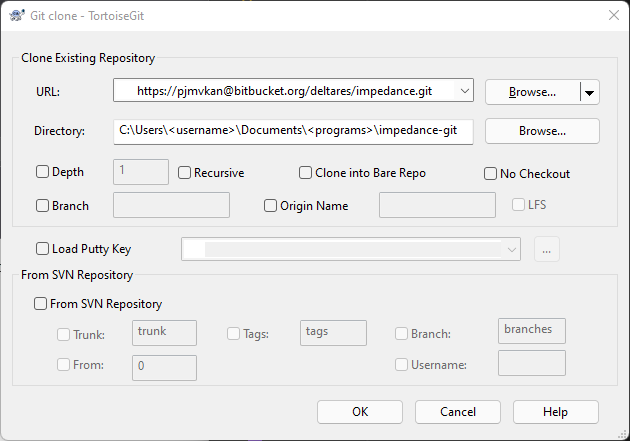
\includegraphics[width=0.6\textwidth]{Figures/Tortoise_clone_impedance}
	\caption{Cloning a repository with TortoiseGit}
	\label{fig:clone}
\end{figure}

\textit{Note}: Running the simulations and tests is best done from the \emph{repository root}. All simulations and tests are designed to find the package, subpackages and configuration files from this directory.

\subsection{Working with the Python code}

Python scripts and programs can only be run by the Python \emph{interpreter}. Installation of this interpreter and other Python \emph{packages} for mathematical operations, basic plotting and file handling, is done by a \emph{package manager} who bundles the packages in an \emph{environment}.

To get things working, follow the instructions in Appendix \ref{appendix:second}.

\begin{itemize}
	\item The commands for creating a dedicated \emph{environment} in Appendix \ref{appendix:config} and \ref{appendix:environments} are listed in Listing \ref{list:impenv}.
\end{itemize}

\lstinputlisting[label=list:impenv,caption=Example textfile with conda commands for new environment, language=Python, linerange={1-100}]{../../environment.txt}

\begin{itemize}
	\item after completion of the dedicated \emph{environment} the Python scripts in the folder "\textsf{twozone\_housemodel-xxxxxxxxxxxx}" or "\textsf{housemodel-git}" can be run in the \textsf{Anaconda Prompt} console.
	\item Alternatively, Python scripts can be run and adapted in an "Integrated development Environment (IDE). The recommended choice is the PyCharm IDE. For installation instructions, follow Appendix \ref{appendix:ide}.
\end{itemize}

\subsection{Package structure}

The repository "\textsf{twozone\_housemodel-git}" contains the modules for the house model. The customary way to organize the modules is to make a \emph{Python package} with \emph{subpackages}. This opens up the possibility of publishing the package on PyPi, so that it can be imported.

See: \url{https://pypi.org/}

From commit \textsf{e74ce58} the files in the \textsf{twozone\_housemodel-git} repository are organized as a package. The proposed structure, implemented in this commit, is:

\dirtree{%
	.1 twozone\_housemodel-git.
	.2 /Documentation.
	.3 /Reference\_Manual.
	.4 \textit{house\_model\_reference\_manual.tex}.
	.4 /Figures.
	.4 /Listings.
	.4 /pdf.
	.5 \textit{this document}.
	.2 \textit{housemodel}.
	.3 \_\_init\_\_.py.
	.3 /basics.
	.4 \_\_init\_\_.py.
	.4 ckf\_tools.py.
	.4 components.py.
	.4 flows.py.
	.4 source\_term.py.
	.4 totalsystem.py.
    .3 /buildings.
	.4 \_\_init\_\_.py.
	.4 building.py.
	.3 controls.
	.4 \_\_init\_\_.py.
	.4 heating\_curves.py.
	.4 Temperature\_SP.py.
	.4 /ivPID.
	.5 PID.py.
	.3 solvers.
	.4 \_\_init\_\_.py.
	.3 sourcesink.
	.4 \_\_init\_\_.py.
	.4 /buffervessels.
	.4 /heatpumps.
	.4 /radiators.
	.3 tools.
	.4 \_\_init\_\_.py.
	.2 tests.
	.3 \_\_init\_\_.py.
	.3 context1.py.
	.3 test\_*.py.
	.2 environment.txt.
	.2 Simulation*.py.
	.2 README.
	.2 setup.py (to be added).
} 

\begin{itemize}
	\item the \emph{repository root} \textsf{twozone\_housemodel-git} contains the simulation scripts and configuration files (for now) 
	\item the \emph{package root} \textsf{housemodel} contains the complete package. This can be seen since it contains an (empty) \textsf{\_\_init\_\_.py} module.
	\item the \emph{subpackage} folders contain the modules with common functions and classes for all simulations. They each contain an (empty) \textsf{\_\_init\_\_.py} module.
	\item a \textsf{tests} folder is placed carefully as a subfolder of the \emph{repository root}. 
	See: \url{https://docs.python-guide.org/writing/structure/} for the underlying philosophy. Here, testing modules (scripts) can be placed. If the names of the test scripts start with \textsf{test\_}, they can be automatically run with the \textsf{pytest} Python package.
\end{itemize}

\textit{Note}: Running the simulations and tests is best done from the \emph{repository root}. All simulations and tests have been updated to find the package, subpackages and configuration files from this directory.

\subsubsection{Subpackage \textsf{basics}}
 The subpackage \textsf{classes} contains the following Python modules:

 \begin{itemize}
	\item \textbf{ckf\_tools.py}. This module contains basic functions to generate the matrices $\mathbf{C^{-1}}$, $\mathbf{K}$ and the source vector $\mathbf{\dot{q}}$.
\end{itemize}

% \lstinputlisting[label=list:constants,caption= Physical Constants in 
% constants.py, language=Python, linerange={2-11}]{Listings/constants.py}
 
 \begin{itemize}
     \item \textbf{components.py}. This module covers the fundamental abstract classes for the network of nodes and edges.
 \end{itemize}
 
% \lstinputlisting[label=list:cells,caption= Class Cell and derived classes in 
% cells.py, language=Python, linerange={2-49}]{Listings/cells.py}

 \begin{itemize}
     \item \textbf{flows.py}. This module contains the \textsf{Flow} class used for generating and updating the convective water flows in the thermal model.
 \end{itemize}
 
% \lstinputlisting[label=list:electrolytes,caption= Class Electrolyte in
% electrolytes.py, language=Python, linerange={2-61}]{Listings/electrolytes.py}

 \begin{itemize}
     \item \textbf{source\_term.py}. This module contains the \textsf{SourceTerm} class used for generating and updating the Fixed Nodes in the thermal model.
 \end{itemize}
 
% \lstinputlisting[label=list:particles,caption= Class Particles in particles.py,
% language=Python, linerange={2-35}]{Listings/particles.py}

 \begin{itemize}
     \item \textbf{totalsystem.py}. This module contains the \textsf{TotalSystem} class which incorporates the complete model expressed in the matrices $\mathbf{C^{-1}}$, $\mathbf{K}$, $\mathbf{F}$, and the source vector $\mathbf{\dot{q}}$. An instance of this class is passed to the model function of the \textsf{scipy.integrate.solve\_ivp} function.
 \end{itemize}
 
% \lstinputlisting[label=list:colloids,caption= Class Colloids in colloids.py,
% language=Python, linerange={2-60}]{Listings/colloids.py}

\subsection{Stratified Buffer Vessel}

The \textsf{StratifiedBuffer} class in the module \textsf{stratified.py} contains the representation of a stratified buffer vessel. The vessel is assumed to have a \emph{cylindrical} shape. Therefore it has the following attributes:

\begin{itemize}
	\item (input) volume $V$ in $m$.
	\item (input) height $h$ in $m$
	\item (input) num\_layers $N$
	\item {layer\_height = $h / N$}
	\item radius $r = \sqrt{[V / (h * \pi)]}$
	\item wall surface of a layer $A_{wall,layer} = 2 * \pi * r * h/N$
	\item $A_{base} = V / h = \pi * r^2$
	\item cap\_layer = $(V / N) * \rho * c_p$
\end{itemize}

\lstinputlisting[label=list:stratified, caption=, language=Python, linerange={178-224}]{../../housemodel/sourcesink/buffervessels/stratified.py}

The \textsf{StratifiedBuffer} class is a central component in the thermal network. Therefore, the class shares the attributes:
\begin{itemize}
	\item \textsf{nodes} of type \textsf{CapacityNode}. \textsf{num\_nodes} equals num\_layers $N$.
	\item \textsf{edges} of type \textsf{CondEdge}. \textsf{num\_edges} equals $N-1$.
	\item a boundary condition \textsf{ambient} representing the indoor surroundings of the buffer vessel.
\end{itemize}

In contrast to the other \textsf{housemodel} classes, the internal capacitive nodes, conductive edges and ambient node, and hence the $\mathbf{C^{-1}}$, $\mathbf{K_{int}}$ and $\mathbf{K_{ext}}$-matrices can be calculated from the input parameters and need not be read from the configuration file. For this purpose the following methods are added to this class:

\begin{itemize}
	\item \textsf{generate\_nodes}
	\item \textsf{generate\_edges}
	\item \textsf{generate\_ambient}
\end{itemize}

The attributes \textsf{begin\_node} and \textsf{end\_node} = \textsf{begin\_node + n\_layers-1} are added to provide the anchor point(s) to the house model.


\newpage

\section{House Model Machine Learning}

\subsection{Introduction}\label{s:introduction}
The developed house model [\url{https://hancse@github.com/hancse/twozone\_housemodel.git}] allows to simulate the heat demand of a given house. Based on weather information such as the outside temperature and solar irradiation, house specifications, and other input factors it is possible to compute the details of the temperature evolution. 

The model needs many details to run. These details will be hard to get a hold of in practice.

It would be interesting to see whether it is possible to use machine learning to abstract from the details that are used to create the model and use only limited amount of input data to create a model that can predict the heat demand of a house. 

 


%\section{Background}\label{s:background}


\subsection{Machine learning approach}\label{s:MLA}


\subsubsection{LSTM network}
We create a Long Short-Term Memory (LSTM) network for predicting the heat demand. An LSTM network is a type of recurrent neural network (RNN). These models are widely used in, for example, the field of speech recognition, language modeling, and machine translation. LSTM networks are also well suited for time series data, as we have here. In a RNN the output of a layer in the network can be fed back to be used as input of an earlier layer in the network. In this way, dependencies on the data history can be taken into account in the model. LSTM networks are a specific type of RNNs, designed such that the network learns which historical data is needed to 
"remember" using the memory cell, and which data can be "forgotten" using a so-termed forget-gate, in order to predict the next output. More background on the working of the LSTM can be found in \cite{LSTM}, a blog by Christopher Olah with a comprehensive explanation of the ideas behind the LSTM network. 

The full network that will be used consists of an LSTM-layer, that is used to learn the dependencies on the historic data, and a fully connected linear layer that applies a linear transformation to the output from the LSTM-layer to obtain the final output, the predicted heat demand. 



\subsubsection{input data selection}

In this first exploration of the potential of using a machine learning model to predict the heat demand of a household we make use of data generated with the house model. The house model can provide a heat demand profile for a full year. The heat demand is based on weather data, temperature and solar irradiation, construction parameters of the house, and some behavioral parameters, such as the number of people present in the house and the thermostat setting.   

The model is described in detail in [ref to document of the house model]. The house is modeled as a network of thermal capacitors, between which energy can be exchanged. The most simple house model uses 2 thermal capacitors, one for the air in the house and one for the walls. Heat can be exchanged between the two capacitors, and the outside air. Essentially this model approximates the house as a single compartment with its walls. 

A more detailed representation of the house can be made by using multiple heat capacitors, for example one for each floor or room.   
Several versions of the specific model have been developed. A first version is created in Matlab-Simulink, and a more elaborate version is under development using Python. 

Initially, we have made use of the data generated by the Matlab-Simulink implementation, which has a time granularity of one hour. Later we have shifted to the more detailed Python implementation of the model, which has more flexibility and a finer time granularity.

The input features we want to use for our model are the same for both the Matlab-Simulink model and the Python model. These should also be easily available in practice. The input features we select to create our model are:
\begin{itemize}
\item Outside temperature ($T_{out}$); we can assume this parameter is easily available through either a local thermometer or an online service providing data of a nearby weather station. Alternatively weather forecast date might be used. 
\item temperature of the house ($T_{house}$); this should be available through the thermostat. In the house model this is the temperature of air. In case of a model that has multiple compartments, we use the air temperature of the main compartment.
\item thermostat set point ($SP$), this should be available though the thermostat. Potentially, these values are even available for future values, since often programs are created to set the thermostat values. 
\item solar irradiation ($Q_{solar}$), although these values may not be straightforward to obtain for a specific location, an estimate value may be obtained from a local weather station. 
\item heat demand ($Q_{demand}$), the historic values of the heat demand will be used to predict the future values. 
\end{itemize}

More features could be available from the house model, such as the heat generated by the appliances and inhabitants or the temperature of the walls. However, not all of these will be practically available. We hope to obtain a machine learned model that can abstract from these details and still give a good prediction for the heat demand for the coming time period. When much data from the house model is needed that is not measured in practice, it is unrealistic the machine learned model could be transferred to a scenario where it works with real life data.  

\textit{NOTE: It might be interesting to also look at the capabilities to predict the house temperature as well. For the other inputs a future value may be obtained from either the weather forecast or the thermostat program. Taking the temperature predictions into account might be helpful for a model predictive control approach?}

\subsubsection{data preprocessing steps}
The input data is loaded from an Excel sheet that contains all the hourly values. When we want to create a model the data needs to be split in a training and a test set. As we are dealing with a time series the order of the data needs to be retained. The first $70\%$ of the data will be used for training the mode and the last $30\%$ will be used for testing. 

Next to splitting the data, the data set needs to be normalized, by subtracting the mean of all feature values ($\mu$) and dividing by the standard deviation ($\sigma$) (using the \texttt{standardscaler}),$x_{norm}= \frac{x-\mu}{\sigma}$. The output is normalized as well.

After the normalization of the data, the data needs to be prepared for the LSTM. From the data a set of sequences is created. For each output value, heat demand at time $t$, a sequence of historical data of input values is needed, time steps $t-N \cdots t-1$.  

\textit{NOTE: the value of N, the number of historical time steps needs to be determined. For the hourly data $N=12$ seems to give good results. A logical choice would be to set $N$ such that 24 hours of historical data is used to predict the next time step, since a high correlation with 24 hours earlier is to be expected. The actual number of time steps depends on the time granularity of the data. 
One may also reason that the heat demand for the next hour is mainly determined by the temperatures and the thermostat setting of the last hour. This implies little history is actually needed.} 

\subsubsection{model training}
In order to train the network, we pass all input data through the network. The mean squared error of the result is computed, and using the Adam-optimizer algorithm the network is improved. The Adam-optimizer is currently one of the most used algorithms, and in many cases gives a faster convergence (check the reference given on https://machinelearningmastery.com/adam-optimization-algorithm-for-deep-learning/). However, it may be useful to investigate the performance of other optimizers.
 
The steps of passing the data through the network and further optimization are repeated for several iterations, or epochs.
 
%
%\begin{itemize}
%\item What are the options for settings for the learning process?
%\item Adam learning algorithm
%\item number of epochs
%\item \ldots
%\end{itemize}
%


\subsubsection{model testing}
After the network has been trained, the obtained model is tested with the test data. The test data consists of the last 30\% of the data sequence obtained from the house model. This data needs to be preprocessed in the same way as the training data. So, we need to scale the data and create the input sequences that are used to predict the next output. 

The output obtained form the network, needs to be scaled back so it can be compared with the real values that have been obtained from the house model. As error metric, we use the RMSE (Root mean squared error). 

\subsubsection{model optimization}
The LSTM network contains several parameters that can be adapted to optimize the learning process, and the quality of the final model.The key parameters are:
\begin{itemize}
\item number of hidden neurons or number of output neurons of the LSTM layer: By increasing this parameter the network complexity is increased. A more complex allows for closer fitting to the training data. However too many hidden neurons may result in an overfitted model. 
\item sequence length: By increasing the sequence length the model takes a larger portion of the history into account for the prediction of the next value. This comes at the cost of a longer computation time. 
\item number of optimization iterations (epochs): By optimizing over more iterations the algorithm has a higher chance to find the optimal model configuration. This comes at the cost of a longer computation time. In general you will see that the gain of model quality is highest in the start of the optimization process. The trade off between increased model accuracy and additional computation time worsens when the number of iterations is large. 
\item learning rate: The learning rate influences the step size that will be taken in the optimization process. This is a parameter that is used by the Adam optimization algorithm. 
\end{itemize}


%\section{Python implementation}
 %various functions
%
%\subsection{LSTM-layer}
%The key parameters that need to be defined for the LSTM-layer are:
%\begin{itemize}
%\item input\_size: the number of input features used for the layer.
%\item hidden\_size: the number of features in the hidden state.
%\end{itemize}
%All other parameters, such as, num\_layers, bias, etc, will be used in the default setting. 
%




\subsection{results}
In this section we look at the first results obtained with the neural network for both the data obtained with the Matlab-Simulink model and the Python model. 



\subsubsection{Matlab-Simulink housemodel}
In this analysis we have trained the model on the data from the Matlab-Simulink model for a light weight construction.  
At the moment of writing this document the specifics on the used input to create the data set are unknown to the author. 

The dataset contains hourly values for the features:
\begin{itemize}
\item temperature\_house: the temperature of the air in the house (in degrees centigrade). 
\item heat\_demand: average power demand to heat the house (in W)
\item setpoint\_temperature: thermostat setpoint (in degrees centigrade)
\item temperature\_outside: the outdoor temperature (in degrees centigrade)
\item heat\_solar: the heat added to the house by the sun (in W), based on the NEN-5060 \cite{NEN5060}. 
\item temperature\_wall: temperature of the walls (in degrees centigrade)
\item heat\_internals: estimate for heat from people and devices present in the house (in W) 
\end{itemize}

From this set we use only the features, temperature\_house, setpoint\_temperature, temperature\_outside, heat\_solar and heat\_demand. 
The LSTM-layer in the network has 20 output nodes, and we use a learning rate of 0.01. Some experimenting shows that after 1000 training epochs little further improvement is made. The obtained model will predict only the next value, i.e., the average heat demand for the next hour, based on the input. 

We vary the input sequence length to see how much history we need to take into account in the training of the model. The results are summarized in Table \ref{tab:results_simulink}. The table shows both the training loss and the test RMSE for various values of the sequence length. The training loss is the MSE of the model on the normalized training data. The RMSE for the test data is based on the real non-normalized heat demand values. \textit{(NOTE: For comparing training and test, it is needed to evaluate them both on the real values.)}

In Table~\ref{tab:results_simulink}, we can see that the best results are obtained for the sequence length of 18. It is likely that the shorter sequence lengths have worse results due to a lack of historical information. For the models with longer sequences the performance might get worse due to the higher model complexity. This implies that training over more iterations is needed to achieve the same level of accuracy. It is also important to note that when the sequence length is increased, the computation time for every iteration in the optimization process is increased as well.
  
\begin{table}[H]
	\centering
		\begin{tabular}{c|c|c}
			\hline
			seq length & train loss & test RMSE  \\
			\hline
			\hline
			2 & 0.256 & 1529\\
			4 & 0.135 & 1562\\
			8 & 0.083	& 681\\
			12 & 0.015 & 316\\	
			16 & 0.014 & 291\\
			18 & 0.011 & 275\\
			24 & 0.010 & 293\\
			32 & 0.013 & 336\\
			\hline
		\end{tabular}
	\caption{training loss and test MSE for varying values of the sequence length}
	\label{tab:results_simulink}
\end{table}


\begin{figure}[H]
	\centering
		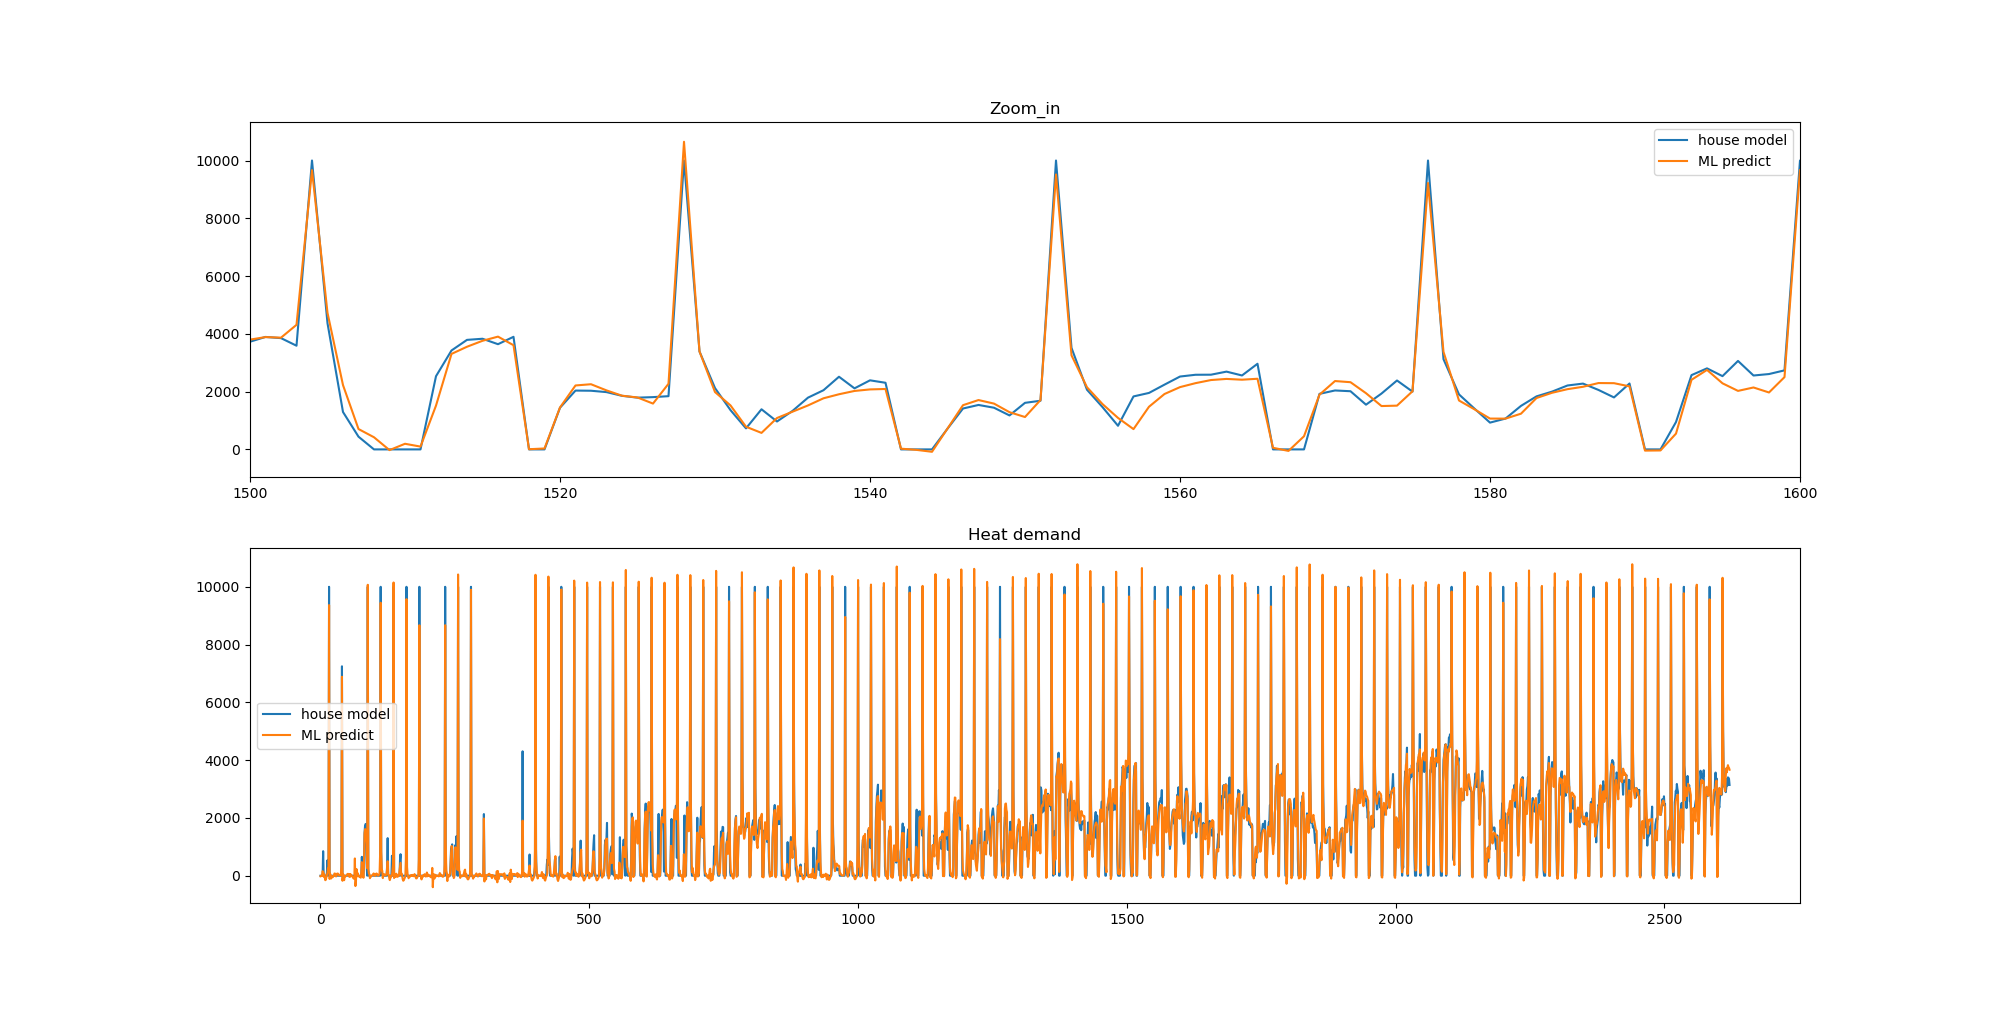
\includegraphics[width = 0.9\textwidth]{figures/seq_18_epoch_1000_Matlab1.png}
		\caption{heat demand for Matlab Simulink model and the ML predictions.}
	\label{fig:matlab_seq18}
\end{figure}

Figure~\ref{fig:matlab_seq18} shows the heat demand according to the Matlab-Simulink model and the ML-predictions when using a sequence length of 18 samples. The figure gives the results for the test set, that is the last 30\% of the year. The x-axis is labeled with the index of the array (corresponding to number of hours after the start), the y-axis is the average heat demand in the hour in W. 

We see that the ML-model matches the general trend of the Matlab-Simulink model. The RMSE of the ML-prediction is 275~W, while the average value is roughly 3000~W. 


\subsubsection{Python house model}
In this analysis we train the data on the Python house model. The data is generated with the version \texttt{Simulation\_for\_companies.py}. This model has a time granularity of 10 minutes, thus 6 values per hour. An excel-file, \texttt{tst\_ML.xlxs}, with output data from the model is generated. The same features as for the Matlab-Simulink model are used: House temperature, thermostat setpoint, outside temperature, solar irradiation and heat demand. Note that, here the solar irradiation is derived from the NEN-5060 global irradiation values \cite{NEN5060}. By interpolation the hourly values from the NEN-5060 are converted to values for every 10 minutes.  

Due to the finer time granularity the ML learning process takes much longer than for the Matlab-Simulink based dataset. First of all, the data set is ten times larger. Furthermore, a larger number of datapoints needs to be used to build the same time span of historical values. Both have a big impact on the computation time. Where the Matlab-Simulink data is trained in a couple of minutes, the Python data takes hours to process on my laptop. 

Furthermore, the model still predicts only for the next time instance. Thus, in for the Python data a prediction for the next 10 minutes interval is made.  

Some explorative experiments have been performed for which the results are summarized in Table \ref{tab:results_python}. Note that the RMSE values are a factor 1000 lower than for the Simulink model. This is due to the fact that the Python model outputs the heat demand in kW instead of W. 

\begin{table}[H]
	\centering
		\begin{tabular}{c|c|c|c}
				\hline
					seq length & nr epochs & train loss & test RMSE  \\
				\hline
				\hline
					24 & 700 & 0.0278 & 0.363 \\
					36 & 1000 & 0.0209	& 0.349 \\
					72 & 700 & 0.0258	& 0.352 \\
					84 & 1000 & 0.0183 & 0.301\\
					144 & 50 & 0.0601 & 0.525\\
					\hline
		\end{tabular}
	\caption{training loss and test RMSE for varying values of the sequence length and number of epochs. }
	\label{tab:results_python}
\end{table}
 

\begin{figure}[H]
	\centering
		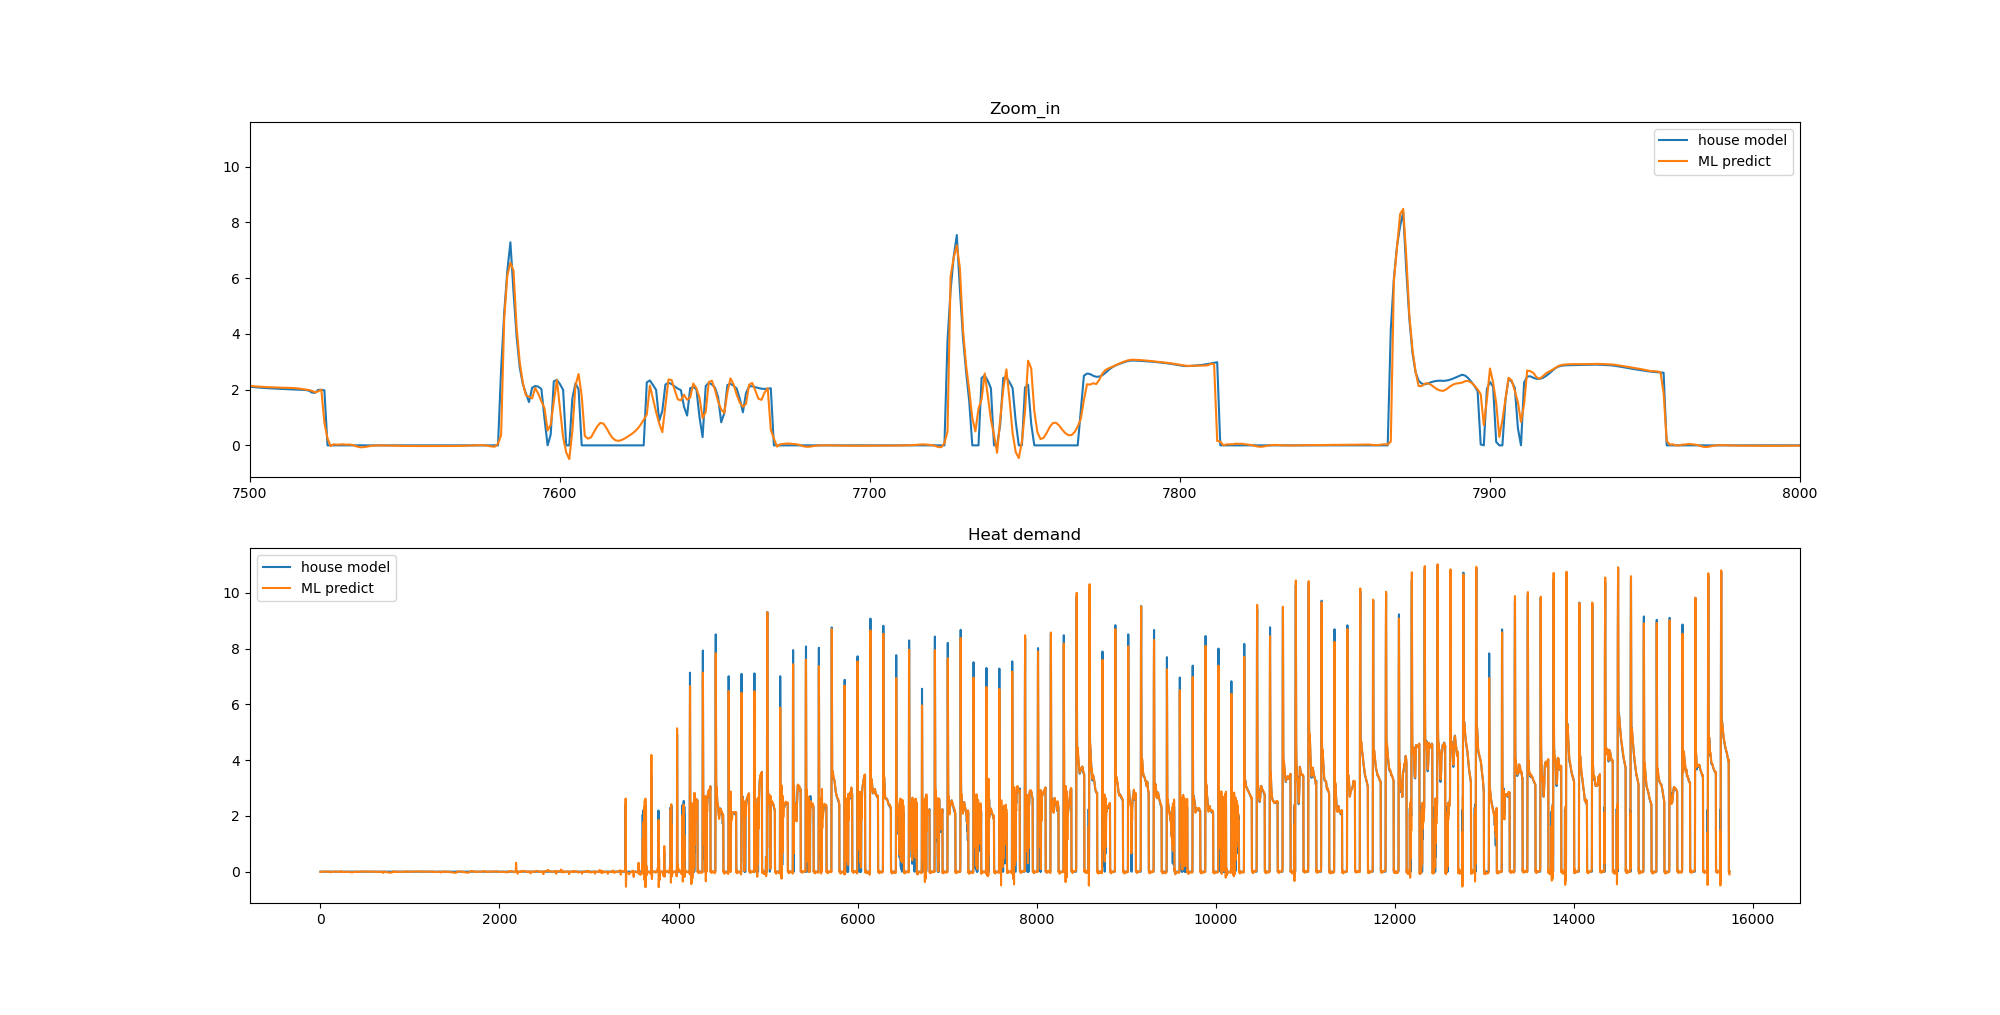
\includegraphics[width = 0.9\textwidth]{figures/seq_84_epoch_1000_Python1.png}
		\caption{heat demand for Matlab Simulink model and the ML predictions.}
	\label{fig:python_seq84}
\end{figure}

In figure \ref{fig:python_seq84} we see the plot of the heat demand according to the Python model and the predictions from the ML-model. Again, the prediction matches the general trend well. However, due to the smaller time granularity, the heat demands contains more variation during the day. This behavior is harder to learn for the ML-model. In some cases the ML-model seems to trail the original data with one time step. Further investigation is needed to see whether the ML-model in these cases mainly reacts on the last value of the heat demand or not. In addition it would be interesting to see whether it is possible to predict the heat demand for a larger time span than only 10 minutes. 

\subsection{conclusion}
The LSTM-network has potential to learn a model that mimics the behavior of the Python house model. However, further research is needed after the initial investigations to get more insight in what the model really can do. Training for over more epochs and with longer historic sequences could give better results.  Also further optimization over the different model parameters is possible. 

Next to optimizing the training process, it would be interesting to further investigate the possibility to predict over a longer time span. Furthermore, it would be interesting to see generic the model is, by looking at predictions for other house configurations. A more general model might be also possible to obtain by training over a wider spectrum of house configurations from the python program. 

Other questions that pop-up:
\begin{itemize}
\item Is it possible to reduce the input, for example can we predict the heat demand without using the history as input?
\item Is it possible to predict the indoor temperature as well? This might be useful for making predictions over a longer time horizon. (weather forecasts and the thermostat program can be used for the other features in the prediction)  
\item Is it possible to use the prediction from the ML model for a model predictive control approach?
\item Would the methodology work on real data from a house? 
\item How much data is needed to train the model sufficiently? Would it be possible to create a "compressed year" with the essential variations on which the model can be trained faster? 
\end{itemize}


\subsection{Python files}
The python files for doing the machine learning are located in the repository, in the directory \texttt{ML\_heat\_demand}. 

\texttt{test\_example.py} will run the machine learning process. Inside this function parameters, like the number of epochs, the number of hidden neurons and the sequence length, can be changed. 

\texttt{load\_and\_preprocess\_training.py} contains the functions that are used for loading and preprocessing the data. 

\texttt{LSTM\_model\_struct.py} builds the LSTM-network, consisting of a LSTM-layer and a fully connect linear layer. 

\texttt{train\_model.py} trains the network on the training data. 

\texttt{Prediction.py} computes the prediction for the test data set. 

The directory \texttt{data} contains the excel input files that were used to create the results in this document, \texttt{test\_excel.xlsx} for the Matlab-Simulink data and \texttt{tst\_ML.xlsx} for the Python model data. Also, the obtained model is saved here as \texttt{test\_model}.



%\bibliography{mybibliography}
\printbibliography[heading=bibintoc, title=References]
\newpage

\begin{appendices}
	\section{Code Management}
\label{app:firstApp}

Coding in a programming language is a process of trial-and-error, leading to a working control program or modelling code in many incremental steps. When working on this individually, but more so when coding in a team of code contributors, tracking progress is mandatory. Also, keeping track of the coding progress in multiple locations reduces the risk of information or code losses.

\subsection{Github or Bitbucket account}
\label{appendix::account}

For optimal collaboration, programmers communicate their last achievement to their colleagues or key users by \textit{committing} them in a \textit{repository} on their local PC, then \textit{pushing} the changes to a central copy of the repository in the cloud. Before starting their work, colleagues can \textit{pull} the last changes, so that their local copy of the repository is up-to-date. The updated local copy is then used for adding new contributions or trying out the updated features. Changes or improvements can be committed locally and pushed to the cloud repository by each member of the team.

For establishing a team and implementing the workflow above, each contributor must have an account on a Git repository cloud service.

\begin{itemize}
	\item Github: Go to \url{https://github.com/} and \emph{sign up} with the button in the upper right corner of the web page.
	\begin{figure}[H]
		\centering
		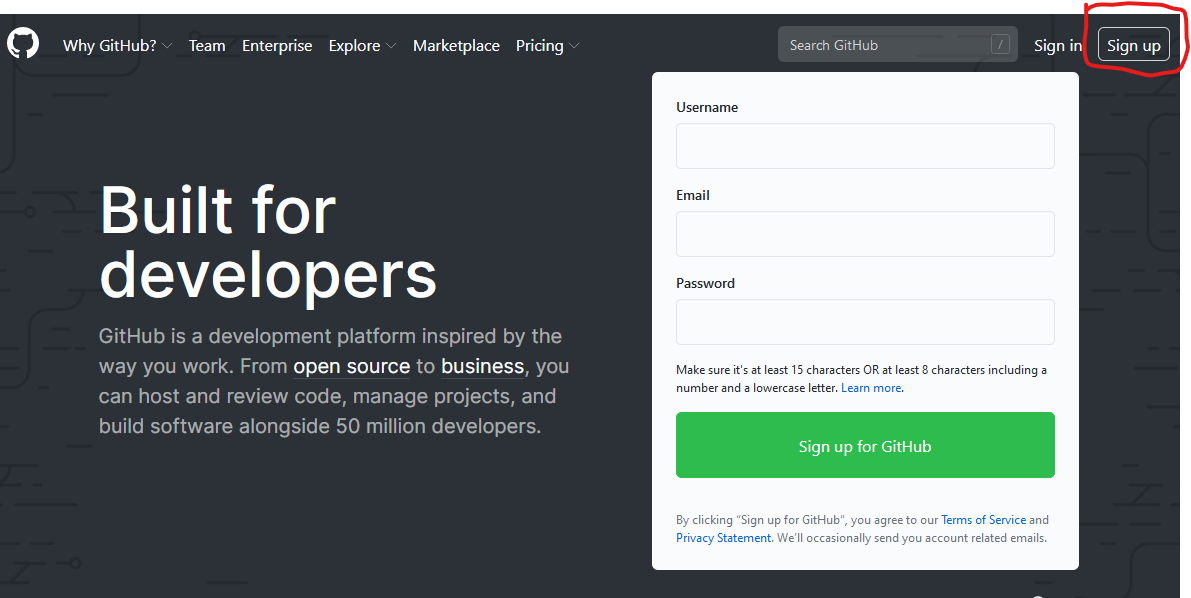
\includegraphics[width=3.0in]{Figures/GitHub_signup.png}
		\caption{GitHub sign-up}
		\label{GitHubSignup}
	\end{figure} 
	\item Bitbucket: Go to \url{https://bitbucket.org/} and sign up with the "Get it free" button in the upper right corner of the web page.
	\begin{figure}[H]
		\centering
		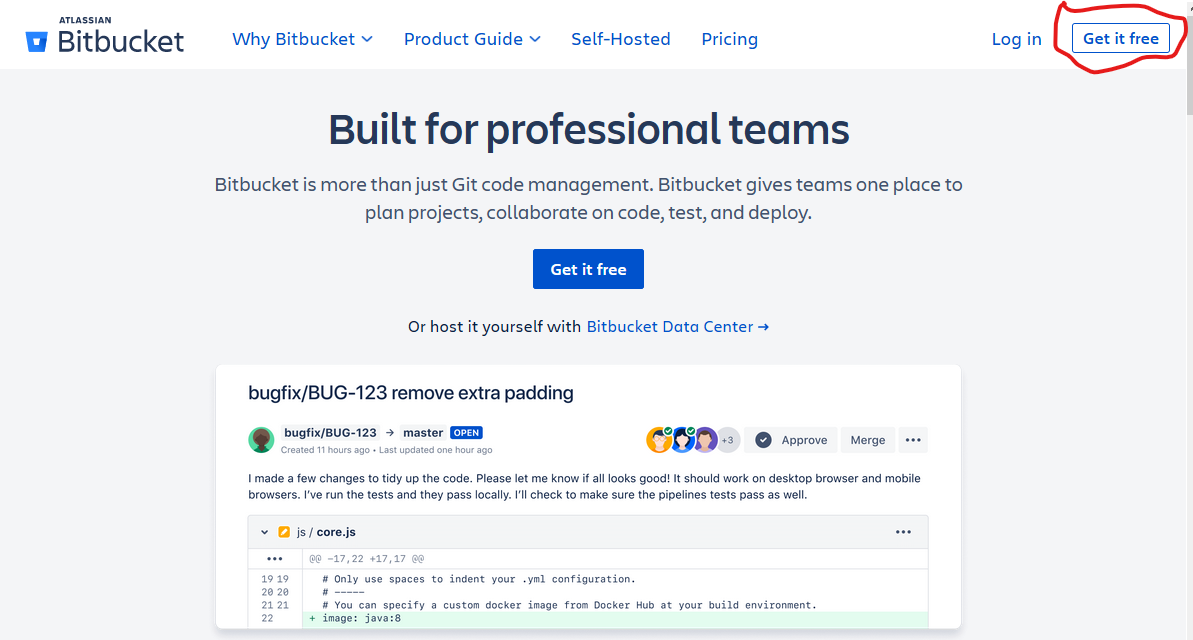
\includegraphics[width=3.0in]{Figures/Bitbucket_signup.png}
		\caption{Bitbucket sign-up}
		\label{BitbucketSignup}
	\end{figure}
\end{itemize}

Do not forget to store your usernames and passwords. The use of a password \textit{vault} is strongly recommended: \url{https://keepass.info/}

\textbf{Note:} Strictly, a GitHub or Bitbucket account is only necessary for all access to \emph{private} repositories or for \emph{contributing} to \emph{public} cloud repositories. Read-only access to \emph{public} repositories is possible without an account.

\subsection{Versioning}
\label{appendix:versioning}

The starting point for version control is the installation of a version control system on your PC. Historically, a number of systems have been invented. Most of them still exist. Among those, CVS, SVN, Bazaar and Mercurial (hg). In the last few years, however, the Git versioning system seems to gain a major "market share". It has been designed by the inventor of Linux, Linus Torvalds, and has a robust performance. The possibilities of Git are a bit overwhelming for the beginning user, which asks for a careful introduction.

\subsubsection{Installation of Git}
On Windows, installation of the \emph{Git for Windows} package is the most convenient option. Download the installer at \url{https://gitforwindows.org/}. 

\begin{figure}[ht]
	\centering
	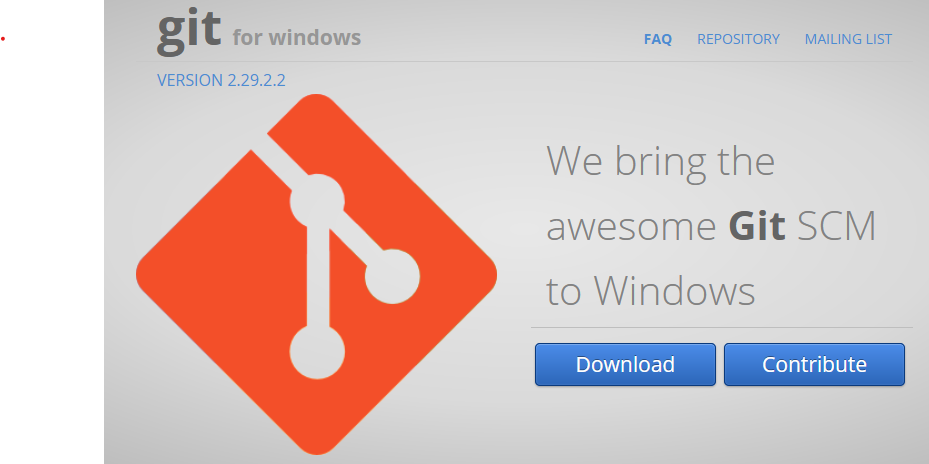
\includegraphics[width=3.0in]{Figures/GitforWindows.png}
	\caption{Git for Windows}
	\label{GitWindows}
\end{figure}

\begin{itemize}
	\item Download the latest version for your OS, which is probably 64-bit \textsf{Git-2.xx.y.z-64-bit.exe}
	\item On execution of the installer, all \emph{default options} can be chosen.
\end{itemize}

On a computer with a Linux OS, there are several options, e.g.:

\begin{itemize}
	\item sudo apt install git (Ubuntu, Debian, RPi)
	\item sudo pacman git (ArchLinux)
\end{itemize}

For Apple Macintosh installation, consult \url{https://git-scm.com/download/mac}.

\subsubsection{Installation of a Git client}

Using Git can be done from the command line (Windows Command Prompt, Git bash or Linux bash). On Linux, this is the preferred option. On Windows, there are useful Git client programs, which make versioning easier after a while. In the beginning, they may just confront you with the overwhelming capacities of Git. Going through this phase merits the effort, however.
A preferred client can be downloaded at \url{https://tortoisegit.org/download/}. 

\begin{itemize}
	\item Download and run the installer: \textsf{TortoiseGit-2.13.0.1-64bit.msi}.
	\item Install with all \emph{default options}.
\end{itemize}

This client integrates with Windows Explorer as an addition to the context menus under the right-mouse-click button.
Installation with the default options is straightforward. Check if the context menus are extended with Git options.

\begin{figure}[ht]
	\centering
	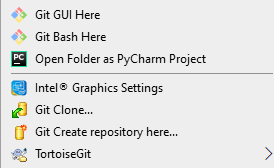
\includegraphics[width=3.0in]{Figures/context_menu.png}
	\caption{Git options in context menu}
	\label{fig:Tortoise_context}
\end{figure}

A second client, with extended functionality can be found at \url{https://www.sourcetreeapp.com/}. Recommended for regular Git users, who work in teams with more than three collaborators, or with collaborators at external reasearch partners. Sourcetree is also available for Mac, but (unfortunately) not for Linux.

\subsubsection{Working with Git}
\label{appendix::gitnotes}

After installation of Git and a Git client, you can start working with Git \emph{repositories}. A repository can be \emph{created} locally, on the harddisk of your PC. Alternatively, a repository from the cloud can be \emph{cloned} to your harddisk. 

After these initial operations, your contributions to the code can be \emph{staged} and \emph{committed} locally and \emph{pushed} to the cloud. Contributions committed and pushed by colleagues can be \emph{pulled} to your local harddisk. 

Regular pulling (before you start coding) and staging-committing-pushing (after you finished coding) cycles will thus assure, that the repositories of all contributors will be synchronized with each other and with the repository in the cloud. The repository in the cloud is often called \emph{origin}.

\textbf{Note:} Each local Git repository should be placed in a separate \emph{local} folder on the physical HDD or SSD. For clarity, it is recommendable to choose a folder name: $\langle repository\_name \rangle$-git. (no spaces in the folder name). 

Each created or cloned repository folder contains a hidden bookkeeping folder named \textsf{.git}. This bookkeeping is not compatible with file sychronization mechanisms. So, please do not create repository folders on Microsoft OneDrive, SharePoint, Teams, Google Drive, OneDrive or SurfDrive shared folders. 

Repository folders are possible on WebDAV, NFS or SMB mounted shared folders, \textbf{if} only one single user has access to the shared folder (from several personal computers, tablets or phones).

\subsection{Git workflow}
\label{appendix:workflow}

\begin{itemize}

\item Creating a repository locally: \url{https://tortoisegit.org/docs/tortoisegit/tgit-dug-create.html}

\item Cloning a repository from GitHub or Bitbucket; \url{https://tortoisegit.org/docs/tortoisegit/tgit-dug-clone.html}

\item Pushing to GitHub or Bitbucket: \url{https://tortoisegit.org/docs/tortoisegit/tgit-dug-push.html}

\item Pulling the changes from the cloud to your local repository: \url{https://tortoisegit.org/docs/tortoisegit/tgit-dug-pull.html}

\item Committing and pushing your local changes to the cloud: \url{https://tortoisegit.org/docs/tortoisegit/tgit-dug-commit.html}
\end{itemize}

\newpage


	\section{Installation of Python and Miniconda}
\label{appendix:second}

Installation of the software for programming in Python on a computer is easiest with a \emph{package manager}. The recommended package manager for Python is named \textsf{conda}. It can be used as a Windows console (\textsf{Anaconda Prompt}), which is very similar to the implementation in a Linux or MacOS X \textsf{bash} console. 
The console program is called \textsf{Miniconda} and can be downloaded at:

\url{https://docs.conda.io/en/latest/miniconda.html}. 
 
Miniconda is available for Windows, Linux and MacOS.
In general, nowadays, one would choose the latest Miniconda Python 3.x version 64-bit installer:\textsf{ Miniconda3-latest-Windows-x86\_64.exe} on Windows, or the analogous installers for Linux and MacOS X.

\begin{itemize}
	\item Download and execute your installer
	\item Install “Just for me”	and create C:\textbackslash Users\textbackslash $\langle username\rangle$\textbackslash miniconda3. Note: $\langle username\rangle$ should NOT contain spaces. Do not install Miniconda system-wide in the "C:\textbackslash Program Files" directory.
	\item Take default options for PATH and REGISTRY update
\end{itemize}

\subsection{Anaconda Prompt}
\label{appendix:anaconda}

After installation of Anaconda (Miniconda) the Windows Start Menu contains a new group "Anaconda3". A detailed view is shown below:

\begin{figure}[H]
	\centering
	\begin{subfigure}[b]{0.38\textwidth}
		\includegraphics[width=\textwidth]{Figures/Anaconda_Prompt.png}
		\caption{Anaconda Start Menu}
		\label{AnacondaMenu}
	\end{subfigure}
	\hfill
	\begin{subfigure}[b]{0.52\textwidth}
		\includegraphics[width=\textwidth]{Figures/AnacondaCommandWindow.png}
		\caption{Anaconda Prompt}
		\label{AnacondaPrompt}
	\end{subfigure}
	\caption{Anaconda (Miniconda) tools installed on Windows}
	\label{AnacondaTools}
\end{figure}

\begin{comment}
	
	\begin{figure}
		\centering
		\begin{minipage}[b]{0.4\textwidth}
			\includegraphics[width=\textwidth]{../images/Anaconda_Prompt.png}
			\caption{Anaconda Start Menu}
			\label{fig:1}
		\end{minipage}
		\hfill
		\begin{minipage}[b]{0.4\textwidth}
			\includegraphics[width=\textwidth]{../images/AnacondaCommandWindow.png}
			\caption{Anaconda Prompt}
			\label{fig:2}
		\end{minipage}
	\end{figure}
	
\end{comment}

The Start Menu entry "\textsf{Anaconda Prompt (miniconda3)}" will open a Windows Command Prompt ("MS-DOS window") with special properties. The current directory name (standard prompt) is preceded by \textsf{(base)}. This is the name of the default \textsf{conda} \emph{environment}.
The \textsf{(base)} environment is \emph{NEVER} used for code development. After installation of the package manager, it contains the latest version of the Python interpreter, which is kept up-to-date with the command:

\textsf{conda update -n base -c defaults conda}

The Python interpreter in the \textsf{(base)} environment may be used by other Windows programs, which will then ask you for the location of the default Python interpreter.

The standard location is: \textsf{C:\textbackslash Users\textbackslash $\langle username\rangle$\textbackslash miniconda3\textbackslash python.exe}.

\subsection{Conda configuration}
\label{appendix:config}

Before creating any dedicated environments, it is recommended to optimize the \textsf{conda} configuration \cite{stack_channels, stack_multiple}. In the previous command, the \textsf{conda} \emph{package} was updated in the \textsf{base} \emph{environment}. The package was read from the \textsf{defaults} \emph{channel}. Other channels exist, that often contain more up-to-date versions of important Python packages. The channel \textsf{conda-forge} is keeping a more recent copy of many packages, including the \textsf{opencv} package, which is a key package used for image analysis. Therefore we add:

\begin{itemize}
	\item \textsf{conda config --show} \qquad this shows the configuration file. Look for "channels:".

    \item \textsf{conda config --add channels conda-forge} \qquad this adds the conda-forge channel before the defaults channel (top of the list).

    \item \textsf{conda config --set channel\_priority strict} \qquad this guarantees that channel priority is maintained according to the list.
\end{itemize}

The config file now shows: \\
... \\
\textsf{channel\_priority: strict \\
	channels: \\
	- conda-forge \\
	- defaults} \\
...

See also: \\
\url{https://stackoverflow.com/questions/39857289/should-conda-or-conda-forge-be-used-for-python-environments} \\
\url{https://conda-forge.org/docs/user/tipsandtricks.html#using-multiple-channels} \\

\subsection{Conda environments}
\label{appendix:environments}

A dedicated environment can be made with the command:

%\sffamily
\textsf{conda create -n $\langle env\_name \rangle$ python=3.x}
%\normalfont

The next commands are:

\textsf{activate $\langle env\_name \rangle$}

\textsf{conda info --envs} or \textsf{conda info -e}: note the active environment with asterisk *

\textsf{conda install $\langle package\_name \rangle$}
or
\textsf{pip install $\langle package\_name \rangle$}

The result can be seen with: \textsf{conda list} : note the packages are all compatible with your Python version

The commands can be stored in a textfile:

\lstinputlisting[label=appendix:envlist,caption=Example textfile with conda commands for new environment, language=Python, linerange={1-100}]{../../environment.txt}

Environments are stored in the private directory of the user. On Windows: 
C:\textbackslash Users\textbackslash $\langle username\rangle$\textbackslash miniconda3\textbackslash envs 

On Linux: /home/$\langle username\rangle$/miniconda3/envs

\textbf{Note:} Code development or storage is NEVER done in C:\textbackslash Users\textbackslash $\langle username\rangle$\textbackslash miniconda3 NOR in any of its subfolders.

\subsection{Python from the console}
\label{appendix:console}

The \textsf{Anaconda Prompt} program on Windows is a specialized version of the general Windows \textsf{Command Prompt}, formerly known as "MS-DOS window" or "console". The advantage of \textsf{Anaconda Prompt} is that all file paths to the Miniconda installation are automatically set and that the prompt indicates the currently active Python environment. On Linux and MacOS, \textsf{Anaconda Prompt} is integrated in the command-line terminal. Thus \textsf{Anaconda Prompt} looks very similar on all operating systems.

Running a Python script in the console is as simple as:

\textsf{activate $\langle env\_name \rangle$}

\textsf{conda info --envs} or \textsf{conda info -e}: note the active environment with asterisk *

\textsf{cd $\langle repository\_root \rangle$}

\textsf{python $\langle script\_name \rangle$}

For an overview of Python command-line features, see:

\url{https://realpython.com/python-command-line-arguments/#the-command-line-interface}

\subsection{Python IDE}
\label{appendix:ide}

\subsubsection{Installation}

\begin{figure}[H]
	\centering
	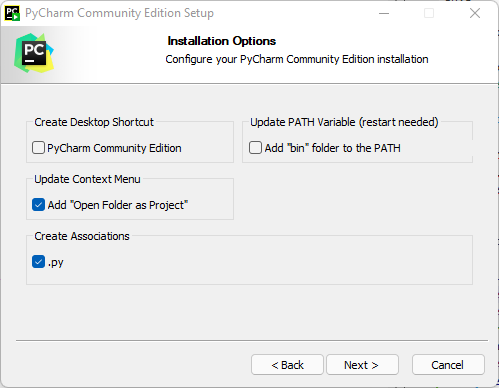
\includegraphics[width=0.5\textwidth]{Figures/PyCharm_checks.png}
	\caption{PyCharm IDE installation on Windows}
	\label{fig:PyCharm}
\end{figure}

After creation of the \textsf{conda} environment with the right selection of Python \emph{packages} for the analysis of the impedance measurements, it is recommended to develop the Python software in a dedicated IDE, where Python scripts can be edited, run, and debugged. The recommended program for this purpose is PyCharm, which can be downloaded here: 

\url{https://www.jetbrains.com/pycharm/download/#section=windows}

\url{https://www.jetbrains.com/community/education/#students}

\begin{itemize}
	\item Download the "Community" installer \textsf{pycharm-community-2021.3.2.exe} and run it.
	\item Install in default directory.
	\item Check options according to Figure~\ref{fig:PyCharm}.
	\item after succesful installation, navigate to the \emph{repository root} folder of your project and right-click on the canvas of the folder window (not on a file or subfolder icon). Choose the "Open Folder as PyCharm Project" item. The PyCharm IDE will start and open the project and subfolders.
	\item Once a project has been opened in PyCharm, it creates a (hidden) subfolder named \textsf{.idea} in the repository root folder. This folder contains the bookkeeping of the IDE. Do not change anything in this \textsf{.idea} subfolder. If anything goes wrong, delete it entirely, and PyCharm will create a fresh one.
	\item 
\end{itemize}

\begin{figure}[H]
	\centering
	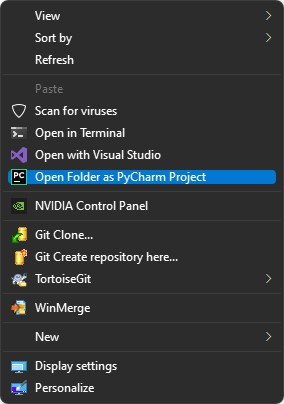
\includegraphics[width=0.3\textwidth]{Figures/context_menu_pycharm.jpg}
	\caption{PyCharm context menu after right-click on root folder canvas}
	\label{fig:contextmenu_pycharm}
\end{figure}

\subsubsection{Configuration}

\begin{itemize}
	\item To work with your Python code in PyCharm, you need to configure a Python interpreter. Assign the Python interpreter from your (existing!) \textsf{conda} environment created following the guidelines in Appendix \ref{appendix:environments} to the open project. See: \url{https://www.jetbrains.com/help/pycharm/configuring-python-interpreter.html}.
	\item After configuring the interpreter, the IDE needs some time to load all the packages from your environment. A progress bar is visible on the bottom of the IDE window.
\end{itemize}

\begin{figure}[H]
	\centering
	\begin{subfigure}[b]{0.45\textwidth}
		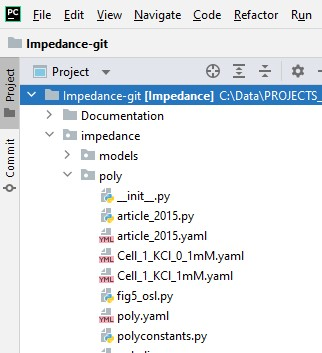
\includegraphics[width=\textwidth]{Figures/project_tab.jpg}
		\caption{Project tab with root folder and subfolders}
		\label{fig:pycharm_projecttab}
	\end{subfigure}
	\hfill
	\begin{subfigure}[b]{0.3\textwidth}
		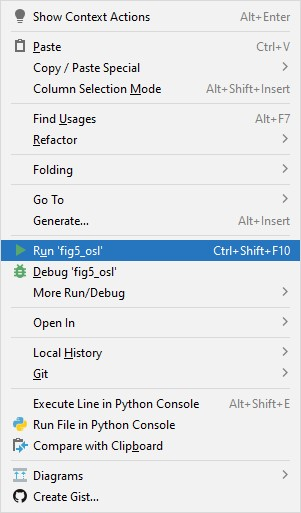
\includegraphics[width=\textwidth]{Figures/run.jpg}
		\caption{Context menu for right-click}
		\label{fig:pycharm_run}
	\end{subfigure}
	\caption{PyCharm project configuration and running}
	\label{fig:pycharm_config}
\end{figure}

\subsubsection{Running and debugging Python scripts}

\begin{itemize}
	\item Selecting a Python script in the Project tab can be done with a left-click. Right-clicking on a Python (*.py) module opens the context menu of Fig.~\ref{fig:pycharm_run}. Clicking the green arrow in the context menu starts executing the selected script.
	\item Double-clicking a *.py module in the Project tab opens the module in the editor window of the IDE. Right-clicking on the canvas of the editor window also opens the context menu of Fig.~\ref{fig:pycharm_run}.
\end{itemize}

\newpage
	\section{Differential equations for stratified buffervessel MvdB}

Python code, for a buffer vessel with 8 layers:
\begin{tiny}
	\begin{equation}
		\begin{aligned}
			dT1 &= ((F_s * (Tsupply - x[0]))          + (F_e * (x[0] - x[1]) * deltaMinus) - (U * As * (x[0] - Tamb)) + ((Aq * lamb) / z) * (x[0] - x[1])) \\
			dT2 &= ((F_e* (x[0] - x[1]) * deltaPlus)  + (F_e * (x[1] - x[2]) * deltaMinus) - (U * As * (x[1] - Tamb)) + ((Aq * lamb) / z) * (x[0] + x[2] - (2 * x[1]))) \\
			dT3 &= ((F_e * (x[1] - x[2]) * deltaPlus) + (F_e * (x[2] - x[3]) * deltaMinus) - (U * As * (x[2] - Tamb)) + ((Aq * lamb) / z) * (x[1] + x[3] - (2 * x[2]))) \\
			dT4 &= ((F_e * (x[2] - x[3]) * deltaPlus) + (F_e * (x[3] - x[4]) * deltaMinus) - (U * As * (x[3] - Tamb)) + ((Aq * lamb) / z) * (x[2] + x[4] - (2 * x[3]))) \\
			dT5 &= ((F_e * (x[3] - x[4]) * deltaPlus) + (F_e * (x[4] - x[5]) * deltaMinus) - (U * As * (x[4] - Tamb)) + ((Aq * lamb) / z) * (x[3] + x[5] - (2 * x[4]))) \\
			dT6 &= ((F_e * (x[4] - x[5]) * deltaPlus) + (F_e * (x[5] - x[6]) * deltaMinus) - (U * As * (x[5] - Tamb)) + ((Aq * lamb) / z) * (x[4] + x[6] - (2 * x[5]))) \\
			dT7 &= ((F_e * (x[5] - x[6]) * deltaPlus) + (F_e * (x[6] - x[7]) * deltaMinus) - (U * As * (x[6] - Tamb)) + ((Aq * lamb) / z) * (x[5] + x[7] - (2 * x[6]))) \\
			dT8 &= ((F_d * (Treturn - x[7]))          + (F_e * (x[6] - x[7]) * deltaPlus)  - (U * As * (x[7] - Tamb)) + ((Aq * lamb) / z) * (x[6] - x[7])) 
		\end{aligned}
	\end{equation}
\end{tiny}

Abbreviations and legend:
\begin{scriptsize}
	\begin{equation}
		\begin{aligned}
			C_x &= m_x \cdot c_{p, w} \qquad \text{for} \quad x =  0 \, \text{...} \, \text{\# of layers}\\
			F_{supply} = F_s &= \dot{m}_{supply} \cdot c_{p, w} \\
			F_{demand} = F_d &= \dot{m}_{demand} \cdot c_{p, w} \\
			\dot{m}_e &= \dot{m}_{supply} - \dot{m}_{demand} \\
			F_e &= \dot{m}_{e} \cdot c_{p, w} \\
			\frac{1}{R_{amb}} &= U \cdot A_s \\
			\frac{1}{R} = \frac{1}{R_{int}} &= \frac{Aq \cdot \lambda}{z}
		\end{aligned}
	\end{equation}
	
	The Python code has a "mismatch" between the range of $dT_1$ (1..8) and the range of $x$ (0 ..7). This is solved by renaming the nodes to $T_{top} \quad T_1 \cdots T_6 \quad T_{bot}$. The set of differential equations the becomes:
	\begin{equation}
		\begin{aligned}
			C_{top} \cdot \frac{dT_{top}}{dt} &= F_s (T_{sup} - T_{top}) &&+ F_e (T_{top} - T_1) \Delta_{\_} &- \frac{1}{R_{amb}} \cdot (T_{top} - T_{amb}) &+ {\color{red}\frac{1}{R} (T_{top} - T_1)} \\
			C_1 \cdot \frac{dT_1}{dt} &= &F_e (T_{top} - T_1) \Delta_{+} &+ F_e (T_1 - T_2) \Delta_{\_} &- \frac{1}{R_{amb}} \cdot (T_1 - T_{amb}) &+ \frac{1}{R} (T_0 + T_2 - 2 T_1) \\
			C_2 \cdot \frac{dT_2}{dt} &= &F_e (T_1 - T_2) \Delta_{+} &+ F_e (T_2 - T_3) \Delta_{\_} &- \frac{1}{R_{amb}} \cdot (T_2 - T_{amb}) &+ \frac{1}{R} (T_1 + T_3 - 2 T_2) \\
			C_3 \cdot \frac{dT_3}{dt} &= &F_e (T_2 - T_3) \Delta_{+} &+ F_e (T_3 - T_4) \Delta_{\_} &- \frac{1}{R_{amb}} \cdot (T_3 - T_{amb}) &+ \frac{1}{R} (T_2 + T_4 - 2 T_3) \\
			C_4 \cdot \frac{dT_4}{dt} &= &F_e (T_3 - T_4) \Delta_{+} &+ F_e (T_4 - T_5) \Delta_{\_} &- \frac{1}{R_{amb}} \cdot (T_4 - T_{amb}) &+ \frac{1}{R} (T_3 + T_5 - 2 T_4) \\
			C_5 \cdot \frac{dT_5}{dt} &= &F_e (T_4 - T_5) \Delta_{+} &+ F_e (T_5 - T_6) \Delta_{\_} &- \frac{1}{R_{amb}} \cdot (T_5 - T_{amb}) &+ \frac{1}{R} (T_4 + T_6 - 2 T_5) \\
			C_6 \cdot \frac{dT_6}{dt} &= &F_e (T_5 - T_6) \Delta_{+} &+ F_e (T_6 - T_7) \Delta_{\_} &- \frac{1}{R_{amb}} \cdot (T_6 - T_{amb}) &+ \frac{1}{R} (T_5 + T_7 - 2 T_6) \\
			C_{bot} \cdot \frac{dT_{bot}}{dt} &= F_d (T_{ret} - T_{bot}) &+ F_e (T_6 - T_{bot}) \Delta_{+} &&- \frac{1}{R_{amb}} (T_{bot} - T_{amb}) &+ \frac{1}{R} (T_6 - T_{bot}) \\
		\end{aligned}
	\end{equation}
	
	Note the term in red in the first equation. There is a sign error...
	
	Converting the set of equations to the form
	
	\begin{subequations}
		\label{eq:matnot}
		\begin{align}
			\mathbf{C} \cdot \boldsymbol{\dot{\theta}} + \mathbf{K} \cdot \boldsymbol{\theta} + \mathbf{F} \cdot \boldsymbol{\theta}= \mathbf{\dot{q}}
		\end{align}
	\end{subequations}
	
	The following set results:
	\begin{equation}
		\begin{aligned}
			C_{top} \cdot \frac{dT_{top}}{dt} &+F_s (T_{top} - T_{sup}) &&+ F_e (T_1 - T_{top}) \Delta_{\_} &+ \frac{1}{R_{amb}} T_{top} &+ {\color{darkgreen}\frac{1}{R} (-T_1 + T_{top})}  &= \frac{1}{R_{amb}} T_{amb} \\
			C_1 \cdot \frac{dT_1}{dt} &= &F_e (T_{top} - T_1) \Delta_{+} &+ F_e (T_1 - T_2) \Delta_{\_} &- \frac{1}{R_{amb}} T_1 &+ \frac{1}{R} (-T_0 -T_2 + 2 T_1) &= \frac{1}{R_{amb}} T_{amb}\\
			C_2 \cdot \frac{dT_2}{dt} &= &F_e (T_1 - T_2) \Delta_{+} &+ F_e (T_2 - T_3) \Delta_{\_} &+ \frac{1}{R_{amb}} T_2 &+ \frac{1}{R} (-T_1 -T_3 + 2 T_2) &= \frac{1}{R_{amb}} T_{amb}\\
			C_3 \cdot \frac{dT_3}{dt} &= &F_e (T_2 - T_3) \Delta_{+} &+ F_e (T_3 - T_4) \Delta_{\_} &+ \frac{1}{R_{amb}} T_3 &+ \frac{1}{R} (-T_2 - T_4 + 2 T_3) &= \frac{1}{R_{amb}} T_{amb}\\
			C_4 \cdot \frac{dT_4}{dt} &= &F_e (T_3 - T_4) \Delta_{+} &+ F_e (T_4 - T_5) \Delta_{\_} &+ \frac{1}{R_{amb}} T_4 &+ \frac{1}{R} (-T_3 - T_5 + 2 T_4) &= \frac{1}{R_{amb}} T_{amb}\\
			C_5 \cdot \frac{dT_5}{dt} &= &F_e (T_4 - T_5) \Delta_{+} &+ F_e (T_5 - T_6) \Delta_{\_} &+ \frac{1}{R_{amb}} T_5 &+ \frac{1}{R} (-T_4 - T_6 + 2 T_5) &= \frac{1}{R_{amb}} T_{amb}\\
			C_6 \cdot \frac{dT_6}{dt} &= &F_e (T_5 - T_6) \Delta_{+} &+ F_e (T_6 - T_7) \Delta_{\_} &+ \frac{1}{R_{amb}} T_6 &+ \frac{1}{R} (-T_5 - T_7 + 2 T_6) &= \frac{1}{R_{amb}} T_{amb}\\
			C_{bot} \cdot \frac{dT_{bot}}{dt} &+ F_d (T_{bot} - T_{ret}) &+ F_e (T_6 - T_{bot}) \Delta_{+} &&+ \frac{1}{R_{amb}} T_{bot} &+ \frac{1}{R} (-T_6 + T_{bot}) &= \frac{1}{R_{amb}} T_{amb}\\
		\end{aligned}
	\end{equation}
	
	Note the correction of the error in the term coloured green. Apparently, the conductive heat loss from the buffervessel to the surroundings is assumed to be equal for \emph{all} layers of the vessel. This translates to a buffer vessel where the top and bottom ends have much better insulation than the side wall.
	
	Writing down the matrix representation of the set we get:
	\begin{equation}
		\mathbf{C} \cdot \boldsymbol{\dot{\theta}} =
		\begin{bmatrix}
			C_{top} & 0 & 0 & 0 & 0 & 0 & 0 & 0 \\
			0 &  C_{1} & 0 & 0 & 0 & 0 & 0 & 0 \\
			0 &  0 & C_{2} & 0 & 0 & 0 & 0 & 0 \\
			0 &  0 & 0 & C_{3} & 0 & 0 & 0 & 0 \\
			0 &  0 & 0 & 0 & C_{4} & 0 & 0 & 0 \\
			0 &  0 & 0 & 0 & 0 & C_{5} & 0 & 0 \\
			0 &  0 & 0 & 0 & 0 & 0 & C_{6} & 0 \\
			0 & 0 & 0 & 0 & 0 & 0 & 0 & C_{bot}
		\end{bmatrix}
		\cdot
		\begin{bmatrix}
			\frac{dT_{top}}{dt} \\
			\frac{dT_{1}}{dt} \\
			\frac{dT_{2}}{dt} \\
			\frac{dT_{3}}{dt} \\
			\frac{dT_{4}}{dt} \\
			\frac{dT_{5}}{dt} \\
			\frac{dT_{6}}{dt} \\
			\frac{dT_{bot}}{dt} \\
		\end{bmatrix}
	\end{equation}
	
	\begin{comment}
		General matrix $\mathbf{K_{int}}$:
		\begin{equation}
			\mathbf{K_{int}} \cdot \boldsymbol{\theta} =
			\begin{bmatrix}
				\frac{1}{R_{1,top}} & \frac{-1}{R_{1,top}} & 0 & 0 & 0 & 0 & 0 & 0 \\
				\frac{-1}{R_{1,top}} &  \frac{1}{R_{1, top}} + \frac{1}{R_{2,1}} & \frac{-1}{R_{2,1}} & 0 & 0 & 0 & 0 & 0 \\
				0 & \frac{-1}{R_{2,1}} &  \frac{1}{R_{2, 1}} + \frac{1}{R_{3,2}} & \frac{-1}{R_{3,2}} & 0 & 0 & 0 & 0 \\
				0 & 0  & \frac{-1}{R_{3,2}} &  \frac{1}{R_{3, 2}} + \frac{1}{R_{4,3}} & \frac{-1}{R_{4,3}} & 0 & 0 & 0 \\
				0 & 0 & 0 & \frac{-1}{R_{4,3}} &  \frac{1}{R_{4, 3}} + \frac{1}{R_{5,4}} & \frac{-1}{R_{5,4}} & 0 & 0 \\
				0 & 0 & 0 & 0 & \frac{-1}{R_{5,4}} &  \frac{1}{R_{5, 4}} + \frac{1}{R_{6,5}} & \frac{-1}{R_{6,5}} & 0 \\
				0 & 0 & 0 & 0 & 0 & \frac{-1}{R_{6,5}} &  \frac{1}{R_{6, 5}} + \frac{1}{R_{bot,6}} & \frac{-1}{R_{bot,6}} \\
				0 & 0 & 0 & 0 & 0 & 0 & \frac{-1}{R_{bot,6}} & \frac{1}{R_{bot,6}}
			\end{bmatrix}
			\cdot
			\begin{bmatrix}
				T_{top} \\
				T_{1} \\
				T_{2} \\
				T_{3} \\
				T_{4} \\
				T_{5} \\
				T_{6} \\
				T_{bot}
			\end{bmatrix}
		\end{equation}
	\end{comment}
	
	Assuming all thermal conductance values between layers are equal as in the Python code:
	\begin{equation}
		\mathbf{K_{int}} \cdot \boldsymbol{\theta} = \frac{1}{R_{int}} \cdot
		\begin{bmatrix}
			1 & -1 & 0 & 0 & 0 & 0 & 0 & 0 \\
			-1 & 2 & -1 & 0 & 0 & 0 & 0 & 0 \\
			0 & -1 & 2 & -1 & 0 & 0 & 0 & 0\\
			0 & 0  & -1 & 2 & -1 & 0 & 0 & 0 \\
			0 & 0 & 0 & -1 &  2 & -1 & 0 & 0 \\
			0 & 0 & 0 & 0 & -1 &  2 & -1 & 0 \\
			0 & 0 & 0 & 0 & 0 & -1 &  2 & -1 \\
			0 & 0 & 0 & 0 & 0 & 0 & -1 & 1
		\end{bmatrix}
		\cdot
		\begin{bmatrix}
			T_{top} \\
			T_{1} \\
			T_{2} \\
			T_{3} \\
			T_{4} \\
			T_{5} \\
			T_{6} \\
			T_{bot}
		\end{bmatrix}
	\end{equation}
	
	\begin{comment}
		General matrix for $\mathbf{K_{ext}}$:
		\begin{equation}
			\mathbf{K_{ext}} \cdot \boldsymbol{\theta} =
			\begin{bmatrix}
				\frac{1}{R_{top, amb}} & 0 & 0 & 0 & 0 & 0 & 0 & 0 \\
				0 &  \frac{1}{R_{1, amb}} & 0 & 0 & 0 & 0 & 0 & 0 \\
				0 & 0 &  \frac{1}{R_{2, amb}} & 0 & 0 & 0 & 0 & 0 \\
				0 & 0  & 0 &  \frac{1}{R_{3, amb}} & 0 & 0 & 0 & 0 \\
				0 & 0 & 0 & 0 &  \frac{1}{R_{4, amb}} & 0 & 0 & 0 \\
				0 & 0 & 0 & 0 & 0 &  \frac{1}{R_{5, amb}} & 0 & 0 \\
				0 & 0 & 0 & 0 & 0 & 0 &  \frac{1}{R_{6, amb}} & 0 \\
				0 & 0 & 0 & 0 & 0 & 0 & 0 & \frac{1}{R_{bot,amb}}
			\end{bmatrix}
			\cdot
			\begin{bmatrix}
				T_{top} \\
				T_{1} \\
				T_{2} \\
				T_{3} \\
				T_{4} \\
				T_{5} \\
				T_{6} \\
				T_{bot}
			\end{bmatrix}
		\end{equation}
	\end{comment}
	
	Assuming conductive heat loss from the buffervessel to the surroundings is equal for \emph{all} layers of the vessel, $\mathbf{K_{ext}}$ becomes:
	\begin{equation}
		\mathbf{K_{ext}} \cdot \boldsymbol{\theta} = \frac{1}{R_{amb}} \cdot
		\begin{bmatrix}
			1 & 0 & 0 & 0 & 0 & 0 & 0 & 0 \\
			0 &  1 & 0 & 0 & 0 & 0 & 0 & 0 \\
			0 & 0 &  1 & 0 & 0 & 0 & 0 & 0 \\
			0 & 0  & 0 &  1 & 0 & 0 & 0 & 0 \\
			0 & 0 & 0 & 0 &  1 & 0 & 0 & 0 \\
			0 & 0 & 0 & 0 & 0 &  1 & 0 & 0 \\
			0 & 0 & 0 & 0 & 0 & 0 &  1 & 0 \\
			0 & 0 & 0 & 0 & 0 & 0 & 0 & 1
		\end{bmatrix}
		\cdot
		\begin{bmatrix}
			T_{top} \\
			T_{1} \\
			T_{2} \\
			T_{3} \\
			T_{4} \\
			T_{5} \\
			T_{6} \\
			T_{bot}
		\end{bmatrix}
	\end{equation}
	
	The $\dot{q}$-vector becomes:
	
	\begin{equation}
		\mathbf{\dot{q}} = 
		\begin{bmatrix}
			\frac{1}{R_{amb}} \cdot T_{amb} \\
			\frac{1}{R_{amb}} \cdot T_{amb} \\
			\frac{1}{R_{amb}} \cdot T_{amb} \\
			\frac{1}{R_{amb}} \cdot T_{amb} \\
			\frac{1}{R_{amb}} \cdot T_{amb} \\
			\frac{1}{R_{amb}} \cdot T_{amb} \\
			\frac{1}{R_{amb}} \cdot T_{amb} \\
			\frac{1}{R_{amb}} \cdot T_{amb}  
		\end{bmatrix}
	\end{equation}
	
	
	\subsubsection{Convective heat transfer in the buffer vessel}
	
	The convective part of the heat transfer equations is:
	\begin{equation}
		\begin{aligned}
			C_{top} \cdot \frac{dT_{top}}{dt} &+F_s T_{top} &&+ F_e (T_1 - T_{top}) \Delta_{\_} &&= F_s T_{sup}\\
			C_1 \cdot \frac{dT_1}{dt} &+ &F_e (T_1 - T_{top}) \Delta_{+} &+ F_e (T_1 - T_2) \Delta_{\_} &= 0 \\
			C_2 \cdot \frac{dT_2}{dt} &+ &F_e (T_2 - T_1) \Delta_{+} &+ F_e (T_2 - T_3) \Delta_{\_} &= 0 \\
			C_3 \cdot \frac{dT_3}{dt} &+ &F_e (T_3 - T_2) \Delta_{+} &+ F_e (T_3 - T_4) \Delta_{\_} &= 0 \\
			C_4 \cdot \frac{dT_4}{dt} &+ &F_e (T_4 - T_3) \Delta_{+} &+ F_e (T_4 - T_5) \Delta_{\_} &= 0 \\
			C_5 \cdot \frac{dT_5}{dt} &+ &F_e (T_5 - T_4) \Delta_{+} &+ F_e (T_5 - T_6) \Delta_{\_} &= 0 \\
			C_6 \cdot \frac{dT_6}{dt} &+ &F_e (T_6 - T_5) \Delta_{+} &+ F_e (T_6 - T_7) \Delta_{\_} &= 0 \\
			C_{bot} \cdot \frac{dT_{bot}}{dt} &+ F_d T_{bot} &+ F_e (T_{bot} - T_6) \Delta_{+} &&= F_d T_{ret}\\
		\end{aligned}
	\end{equation}
	
	If $\dot{m}_e = \dot{m}_{supply} - \dot{m}_{demand} > 0$, $\Delta_{+} = 1$ and $ \Delta_{\_} = 0 $.
	\begin{equation}
		\begin{aligned}
			C_{top} \cdot \frac{dT_{top}}{dt} &+ F_s T_{top} &= F_s T_{sup}\\
			C_1 \cdot \frac{dT_1}{dt} & + &F_e \cdot (T_1 - T_{top}) \cdot \Delta_{+} = 0 \\
			C_2 \cdot \frac{dT_2}{dt} &+ &F_e \cdot (T_2 - T_1) \cdot \Delta_{+} = 0 \\
			C_3 \cdot \frac{dT_3}{dt} &+ &F_e \cdot (T_3 - T_2) \cdot \Delta_{+} = 0 \\
			C_4 \cdot \frac{dT_4}{dt} &+ &F_e \cdot (T_4 - T_3) \cdot \Delta_{+} = 0\\
			C_5 \cdot \frac{dT_5}{dt} &+ &F_e \cdot (T_5 - T_4) \cdot \Delta_{+} = 0\\
			C_6 \cdot \frac{dT_6}{dt} &+ &F_e \cdot (T_6 - T_5) \cdot \Delta_{+} = 0\\
			C_{bot} \cdot \frac{dT_{bot}}{dt} &+ F_d T_{bot} + & F_e (T_{bot} - T_6) \Delta_{+}  = F_d T_{ret}\\
		\end{aligned}
	\end{equation}
	
	\begin{equation}
		\mathbf{F} =  
		\begin{bmatrix}
			F_e & 0 & 0 & 0 & 0 & 0 & 0 & -F_e \\
			-F_e &F_e & 0 & 0 & 0 & 0 & 0 & 0 \\
			0 & -F_e & F_e & 0 & 0 & 0 & 0 & 0 \\
			0 & 0 & -F_e & F_e & 0 & 0 & 0 & 0 \\
			0 & 0 & 0 & -F_e & F_e & 0 & 0 & 0 \\
			0 & 0 & 0 & 0 & -F_e & F_e & 0 & 0 \\
			0 & 0 & 0 & 0 & 0 & -F_e & F_e & 0 \\
			0 & 0 & 0 & 0 & 0 & 0 & -F_e & F_e
		\end{bmatrix}
		\label{eq:flowmatrix}
	\end{equation}
	
	If $\dot{m}_e = \dot{m}_{supply} - \dot{m}_{demand} < 0$, $\Delta_{+} = 0$ and $ \Delta_{\_} = 1 $.
	\begin{equation}
		\begin{aligned}
			C_{top} \cdot \frac{dT_{top}}{dt} &+F_s T_{top} &+ F_e (T_1 - T_{top}) \Delta_{\_} &= F_s T_{sup}\\
			C_1 \cdot \frac{dT_1}{dt} &&+ F_e (T_2 - T_1) \Delta_{\_} &= 0 \\
			C_2 \cdot \frac{dT_2}{dt} &&+ F_e (T_3 - T_2) \Delta_{\_} &= 0 \\
			C_3 \cdot \frac{dT_3}{dt} &&+ F_e (T_4 - T_3) \Delta_{\_} &= 0 \\
			C_4 \cdot \frac{dT_4}{dt} &&+ F_e (T_5 - T_4) \Delta_{\_} &= 0 \\
			C_5 \cdot \frac{dT_5}{dt} &&+ F_e (T_6 - T_5) \Delta_{\_} &= 0 \\
			C_6 \cdot \frac{dT_6}{dt} &&+ F_e (T_7 - T_6) \Delta_{\_} &= 0 \\
			C_{bot} \cdot \frac{dT_{bot}}{dt} &+ F_d T_{bot} &&= F_d T_{ret}\\
		\end{aligned}
	\end{equation}
	
	\begin{equation}
		\mathbf{F} =  
		\begin{bmatrix}
			-F_e & F_e & 0 & 0 & 0 & 0 & 0 & 0 \\
			0 & -F_e & F_e & 0 & 0 & 0 & 0 & 0 \\
			0 & 0 & -F_e & F_e & 0 & 0 & 0 & 0 \\
			0 & 0 & 0 & -F_e & F_e & 0 & 0 & 0 \\
			0 & 0 & 0 & 0 & -F_e & F_e & 0 & 0 \\
			0 & 0 & 0 & 0 & 0 & -F_e & F_e & 0 \\
			0 & 0 & 0 & 0 & 0 & 0 & -F_e & F_e \\
			F_e & 0 & 0 & 0 & 0 & 0 & 0 & -F_e
		\end{bmatrix}
		\label{eq:flowmatrix}
	\end{equation}
	
	Note that since $\dot{m}_e = \dot{m}_{supply} - \dot{m}_{demand} < 0$, the diagonal elements of th $\mathbf{F}$-matrix are positive, like in the case $\dot{m}_e > 0$
	
	Derivation $\mathbf{F}$-matrices:
	
	Directed supply flow: $F_{supply}$ : [top 1 2 3 4 5 6 bottom top]
	
	Directed demand flow: $F_{demand}$ : [bottom 6 5 4 3 2 1 top bottom]
	
	\begin{equation}
		\mathbf{DF_{supply}} \cdot \boldsymbol{\theta} =
		\begin{bmatrix}
			0 & 1 & 0 & 0 & 0 & 0 & 0 & -1 \\
			-1 & 0 & 1 & 0 & 0 & 0 & 0 & 0 \\
			0 & -1 & 0 & 1 & 0 & 0 & 0 & 0 \\
			0 & 0 & -1 & 0 & 1 & 0 & 0 & 0 \\
			0 & 0 & 0 & -1 & 0 & 1 & 0 & 0 \\
			0 & 0 & 0 & 0 & -1 & 0 & 1 & 0 \\
			0 & 0 & 0 & 0 & 0 & -1 & 0 & 1 \\
			1 & 0 & 0 & 0 & 0 & 0 & -1 & 0
		\end{bmatrix}
		\cdot
		\begin{bmatrix}
			T_{top} \\
			T_{1} \\
			T_{2} \\
			T_{3} \\
			T_{4} \\
			T_{5} \\
			T_{6} \\
			T_{bot}
		\end{bmatrix}
	\end{equation}
	
	\begin{equation}
		\mathbf{DF_{demand}} \cdot \boldsymbol{\theta} =
		\begin{bmatrix}
			0 & -1 & 0 & 0 & 0 & 0 & 0 & 1 \\
			1 & 0 & -1 & 0 & 0 & 0 & 0 & 0 \\
			0 & 1 & 0 & -1 & 0 & 0 & 0 & 0 \\
			0 & 0 & 1 & 0 & -1 & 0 & 0 & 0 \\
			0 & 0 & 0 & 1 & 0 & -1 & 0 & 0 \\
			0 & 0 & 0 & 0 & 1 & 0 & -1 & 0 \\
			0 & 0 & 0 & 0 & 0 & 1 & 0 & -1 \\
			-1 & 0 & 0 & 0 & 0 & 0 & 1 & 0
		\end{bmatrix}
		\cdot
		\begin{bmatrix}
			T_{top} \\
			T_{1} \\
			T_{2} \\
			T_{3} \\
			T_{4} \\
			T_{5} \\
			T_{6} \\
			T_{bot}
		\end{bmatrix}
	\end{equation}
	
	\begin{equation}
		\mathbf{SF} = f_s \cdot \mathbf{DF_{supply}} + f_d \cdot \mathbf{DF_{demand}} = 
		\begin{bmatrix}
			0 & \dot{f_s}-\dot{f_d} & 0 & 0 & 0 & 0 & 0 & \dot{f_d}-\dot{f_s} \\
			\dot{f_d}-\dot{f_s} & 0 & \dot{f_s}-\dot{f_d} & 0 & 0 & 0 & 0 & 0 \\
			0 & \dot{f_d}-\dot{f_s} & 0 & \dot{f_s}-\dot{f_d} & 0 & 0 & 0 & 0 \\
			0 & 0 & \dot{f_d}-\dot{f_s} & 0 & \dot{f_s}-\dot{f_d} & 0 & 0 & 0 \\
			0 & 0 & 0 & \dot{f_d}-\dot{f_s} & 0 & \dot{f_s}-\dot{f_d} & 0 & 0 \\
			0 & 0 & 0 & 0 & \dot{f_d}-\dot{f_s} & 0 & \dot{f_s}-\dot{f_d} & 0 \\
			0 & 0 & 0 & 0 & 0 & \dot{f_d}-\dot{f_s} & 0 & \dot{f_s}-\dot{f_d} \\
			\dot{f_s}-\dot{f_d} & 0 & 0 & 0 & 0 & 0 & \dot{f_d}-\dot{f_s} & 0
		\end{bmatrix}
		\label{eq:addbufferflows}
	\end{equation}
	
	Since we want an $\mathbf{F}$-matrix on the left-hand side of the differential equations, the correct elements are obtained by taking the $\text{min}(\mathbf{SF},0)$, here we mean for each element in $\mathbf{SF}$ we take the minimum of the respective element and 0. 
	Thus, in the case $f_s>f_d$ the elements $\dot{f_s}-\dot{f_d} > 0 $ are replaced by 0 and the elements $\dot{f_d}-\dot{f_s} < 0 $ remain. The matrix $\text{min}(\mathbf{SF},0)$ will become:
	\begin{equation}
		\text{min}(\mathbf{SF},0) = 
		\begin{bmatrix}
			0 & 0 & 0 & 0 & 0 & 0 & 0 & \dot{f_d}-\dot{f_s} \\
			\dot{f_d}-\dot{f_s} & 0 & 0 & 0 & 0 & 0 & 0 & 0 \\
			0 & \dot{f_d}-\dot{f_s} & 0 & 0 & 0 & 0 & 0 & 0 \\
			0 & 0 & \dot{f_d}-\dot{f_s} & 0 & 0 & 0 & 0 & 0 \\
			0 & 0 & 0 & \dot{f_d}-\dot{f_s} & 0 & 0 & 0 & 0 \\
			0 & 0 & 0 & 0 & \dot{f_d}-\dot{f_s} & 0 & 0 & 0 \\
			0 & 0 & 0 & 0 & 0 & \dot{f_d}-\dot{f_s} & 0 & 0 \\
			0 & 0 & 0 & 0 & 0 & 0 & \dot{f_d}-\dot{f_s} & 0
		\end{bmatrix}
		\label{eq:minSFzero_8}
	\end{equation}
	
	Now, the diagonal elements can be computed. The diagonal elements are equal to minus the sum of the off-diagonal elements in their respective row. For the matrix given in equation \ref{eq:minSFzero_8} this results in the flow matrix $\mathbf{F}$:
	\begin{equation}
		\mathbf{F} =  
		\begin{bmatrix}
			-(\dot{f_d}-\dot{f_s}) & 0 & 0 & 0 & 0 & 0 & 0 & \dot{f_d}-\dot{f_s} \\
			\dot{f_d}-\dot{f_s} & -(\dot{f_d}-\dot{f_s}) & 0 & 0 & 0 & 0 & 0 & 0 \\
			0 & \dot{f_d}-\dot{f_s} & -(\dot{f_d}-\dot{f_s}) & 0 & 0 & 0 & 0 & 0 \\
			0 & 0 & \dot{f_d}-\dot{f_s} & -(\dot{f_d}-\dot{f_s}) & 0 & 0 & 0 & 0 \\
			0 & 0 & 0 & \dot{f_d}-\dot{f_s} & -(\dot{f_d}-\dot{f_s}) & 0 & 0 & 0 \\
			0 & 0 & 0 & 0 & \dot{f_d}-\dot{f_s} & -(\dot{f_d}-\dot{f_s}) & 0 & 0 \\
			0 & 0 & 0 & 0 & 0 & \dot{f_d}-\dot{f_s} & -(\dot{f_d}-\dot{f_s}) & 0 \\
			0 & 0 & 0 & 0 & 0 & 0 & \dot{f_d}-\dot{f_s} & -(\dot{f_d}-\dot{f_s})
		\end{bmatrix}
		\label{eq:flowmatrix}
	\end{equation}
	
	If the supply and demand flows in the buffervessel are carried by the same liquid medium (water), a differential mass flow $\dot{m}_e = \dot{m}_{supply} - \dot{m}_{demand}$ can be defined, and 
	$ F_e = \dot{m}_{e} \cdot c_{p, w} = \dot{f_s}-\dot{f_d}$. The matrix $\mathbf{F}$ becomes:
	
	\begin{equation}
		\mathbf{F} =  
		\begin{bmatrix}
			F_e & 0 & 0 & 0 & 0 & 0 & 0 & -F_e \\
			-F_e &F_e & 0 & 0 & 0 & 0 & 0 & 0 \\
			0 & -F_e & F_e & 0 & 0 & 0 & 0 & 0 \\
			0 & 0 & -F_e & F_e & 0 & 0 & 0 & 0 \\
			0 & 0 & 0 & -F_e & F_e & 0 & 0 & 0 \\
			0 & 0 & 0 & 0 & -F_e & F_e & 0 & 0 \\
			0 & 0 & 0 & 0 & 0 & -F_e & F_e & 0 \\
			0 & 0 & 0 & 0 & 0 & 0 & -F_e & F_e
		\end{bmatrix}
		\label{eq:flowmatrix}
	\end{equation}
	
	In the case $f_s < f_d$ the elements $\dot{f_d}-\dot{f_s} > 0 $ are replaced by 0 and the elements $\dot{f_s}-\dot{f_d} < 0 $ remain. The matrix $\text{min}(\mathbf{SF},0)$ will become:
	\begin{equation}
		\text{min}(\mathbf{SF},0) = 
		\begin{bmatrix}
			0 & \dot{f_s}-\dot{f_d} & 0 & 0 & 0 & 0 & 0 & 0 \\
			0 & 0 & \dot{f_s}-\dot{f_d} & 0 & 0 & 0 & 0 & 0 \\
			0 & 0 & 0 & \dot{f_s}-\dot{f_d} & 0 & 0 & 0 & 0 \\
			0 & 0 & 0 & 0 & \dot{f_s}-\dot{f_d} & 0 & 0 & 0 \\
			0 & 0 & 0 & 0 & 0 & \dot{f_s}-\dot{f_d} & 0 & 0 \\
			0 & 0 & 0 & 0 & 0 & 0 & \dot{f_s}-\dot{f_d} & 0 \\
			0 & 0 & 0 & 0 & 0 & 0 & 0 & \dot{f_s}-\dot{f_d} \\
			\dot{f_s}-\dot{f_d} & 0 & 0 & 0 & 0 & 0 & 0 & 0
		\end{bmatrix}
		\label{eq:minSFzero_8}
	\end{equation}
	
	Now, the diagonal elements can be computed. The diagonal elements are equal to minus the sum of the off-diagonal elements in their respective row. For the matrix given in equation \ref{eq:minSFzero_8} this results in the flow matrix $\mathbf{F}$:
	\begin{equation}
		\mathbf{F} =  
		\begin{bmatrix}
			-(\dot{f_s}-\dot{f_d}) & \dot{f_s}-\dot{f_d} & 0 & 0 & 0 & 0 & 0 & 0 \\
			0 & -(\dot{f_s}-\dot{f_d}) & \dot{f_s}-\dot{f_d} & 0 & 0 & 0 & 0 & 0 \\
			0 & 0 & -(\dot{f_s}-\dot{f_d}) & \dot{f_s}-\dot{f_d} & 0 & 0 & 0 & 0 \\
			0 & 0 & 0 & -(\dot{f_s}-\dot{f_d}) & \dot{f_s}-\dot{f_d} & 0 & 0 & 0 \\
			0 & 0 & 0 & 0 & -(\dot{f_s}-\dot{f_d}) & \dot{f_s}-\dot{f_d} & 0 & 0 \\
			0 & 0 & 0 & 0 & 0 & -(\dot{f_s}-\dot{f_d}) & \dot{f_s}-\dot{f_d} & 0 \\
			0 & 0 & 0 & 0 & 0 & 0 & -(\dot{f_s}-\dot{f_d}) & \dot{f_s}-\dot{f_d} \\
			\dot{f_s}-\dot{f_d} & 0 & 0 & 0 & 0 & 0 & 0 & -(\dot{f_s}-\dot{f_d})
		\end{bmatrix}
		\label{eq:flowmatrix}
	\end{equation}
	
	If the supply and demand flows in the buffervessel are carried by the same liquid medium (water), a differential mass flow $\dot{m}_e = \dot{m}_{supply} - \dot{m}_{demand}$ can be defined, and 
	$ F_e = \dot{m}_{e} \cdot c_{p, w} = \dot{f_s}-\dot{f_d}$. The matrix $\mathbf{F}$ becomes:
	
	\begin{equation}
		\mathbf{F} =  
		\begin{bmatrix}
			-F_e & F_e & 0 & 0 & 0 & 0 & 0 & 0 \\
			0 & -F_e & F_e & 0 & 0 & 0 & 0 & 0 \\
			0 & 0 & -F_e & F_e & 0 & 0 & 0 & 0 \\
			0 & 0 & 0 & -F_e & F_e & 0 & 0 & 0 \\
			0 & 0 & 0 & 0 & -F_e & F_e & 0 & 0 \\
			0 & 0 & 0 & 0 & 0 & -F_e & F_e & 0 \\
			0 & 0 & 0 & 0 & 0 & 0 & -F_e & F_e \\
			F_e & 0 & 0 & 0 & 0 & 0 & 0 & -F_e
		\end{bmatrix}
		\label{eq:flowmatrix}
	\end{equation}
	
\end{scriptsize}

\newpage
	\section{Documentation buffervessel MvdB}

\subsection{Introduction}

This document describes the buffer vessel model that can be incorporated into the HAN dynamic house model.

\textbf{List of symbols:}

\begin{itemize}
    \item [$m$] {mass [kg]}
    \item [$\dot{m}$] {mass flow [kg/s]}
    \item [$C_w$] {Specific heat of water [J/kg]}
    \item [$T$] {Temperature [C]}
    \item [$U$] {Thermal transmittance [W/K]}
    \item [$A$] {Area [\(m^2\)]}
    \item [$\lambda$] {Heat conductivity [W/mK]}
\end{itemize}

\subsection{Model description}

The model for the buffer vessel is derived from the paper of Rakesh Sinha et al. \cite{sinha2020flexibility}

The model consists of a heating element, located outside of the buffer vessel, which can take water from the vessel and heat the water to a desired temperature.The hot water is then injected to the top of the buffer vessel. 

Hot water is is taken from the top of the buffer vessel on the demand side. Cooled water coming from the load is returned tot the bottom of the vessel.

A schematic description of the buffer vessel is shown below.

\begin{figure}[H]
	\centering
	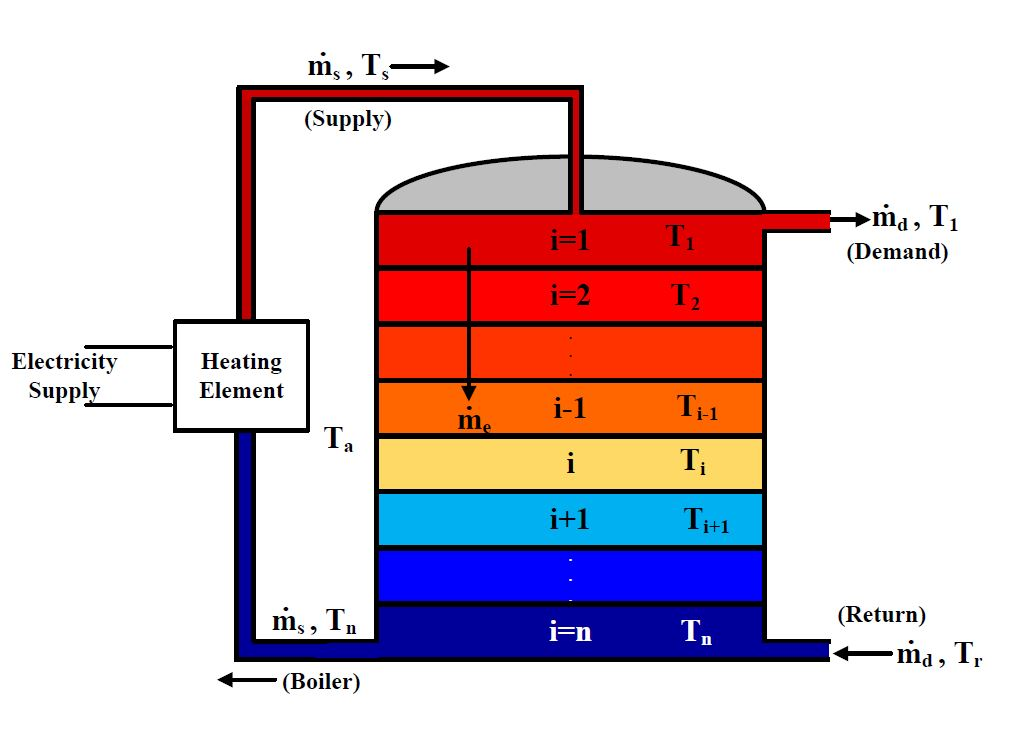
\includegraphics[width=0.8\columnwidth]{Figures/buffervessel_setup.JPG}
	\caption[Short title]{Buffer vessel representation}
\end{figure}

Due to the fact that the density of water decreases with temperature above 4 $\degC$, different temperature layers are created.

In order to model this, the buffer vessel will be divided into $N$ different sections 


\subsection{Mathematical description}

For the top layer:

\begin{equation}
	\label{eq:Buffer vessel top layer}
	mC_w \dfrac{dT_1}{dt} = \dot{m_s}C_w(T_s - T_1) + \dot{m_e}C_w(T_1 - T_2)*sgn(\dot{-m_e}) - UA_s(T_1 - T_a) - \frac{A_q\lambda_w}{z}(T_1-T_2)
\end{equation}

For the middle layers:

\begin{equation}
	\label{eq:Buffer vessel middle layers}
	mC_w \dfrac{dT_i}{dt} = \dot{m_e}C_w(T_{i-1} - T_{i})*sgn(\dot{m_e}) + \dot{m_e}C_w(T_{i} - T_{i+1})*sgn(\dot{-m_e}) - UA_s(T_i - T_a) + \frac{A_q\lambda_w}{z}(T_{i-1} + T_{i+1} - 2T_i)
\end{equation}

For the bottom layer:

\begin{equation}
	\label{eq:Buffer vessel bottom layer}
	mC_w \dfrac{dT_n}{dt} = \dot{m_d}C_w(T_r - T_n) + \dot{m_e}C_w(T_{n-1} - T_n)*sgn(\dot{m_e}) - UA_s(T_n + T_a) + \frac{A_q\lambda_w}{z}(T_{n-1}-T_n)
\end{equation}

\newpage

\subsection{Validation}

To check to model from the paper, the following parameters are used:

\begin{figure}[h]
	\centering
	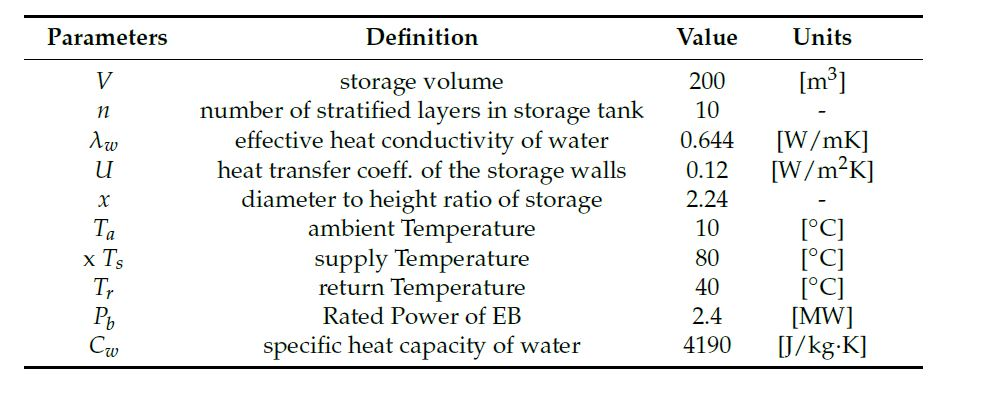
\includegraphics[width=0.7\columnwidth]{Figures/parameters_paper.JPG}
	\caption[Short title]{Buffer vessel parameters}
\end{figure}

This results in the following graph:

\begin{figure}[H]
	\centering
	\subfloat[\centering paper results]{{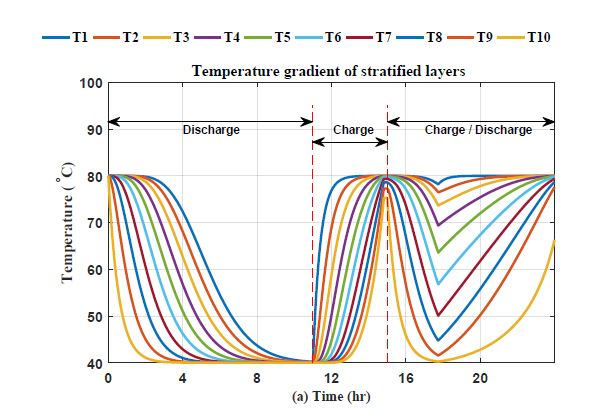
\includegraphics[width=0.7\columnwidth]{Figures/paper_results.jpg} }}
	\qquad
	\subfloat[\centering Python results]{{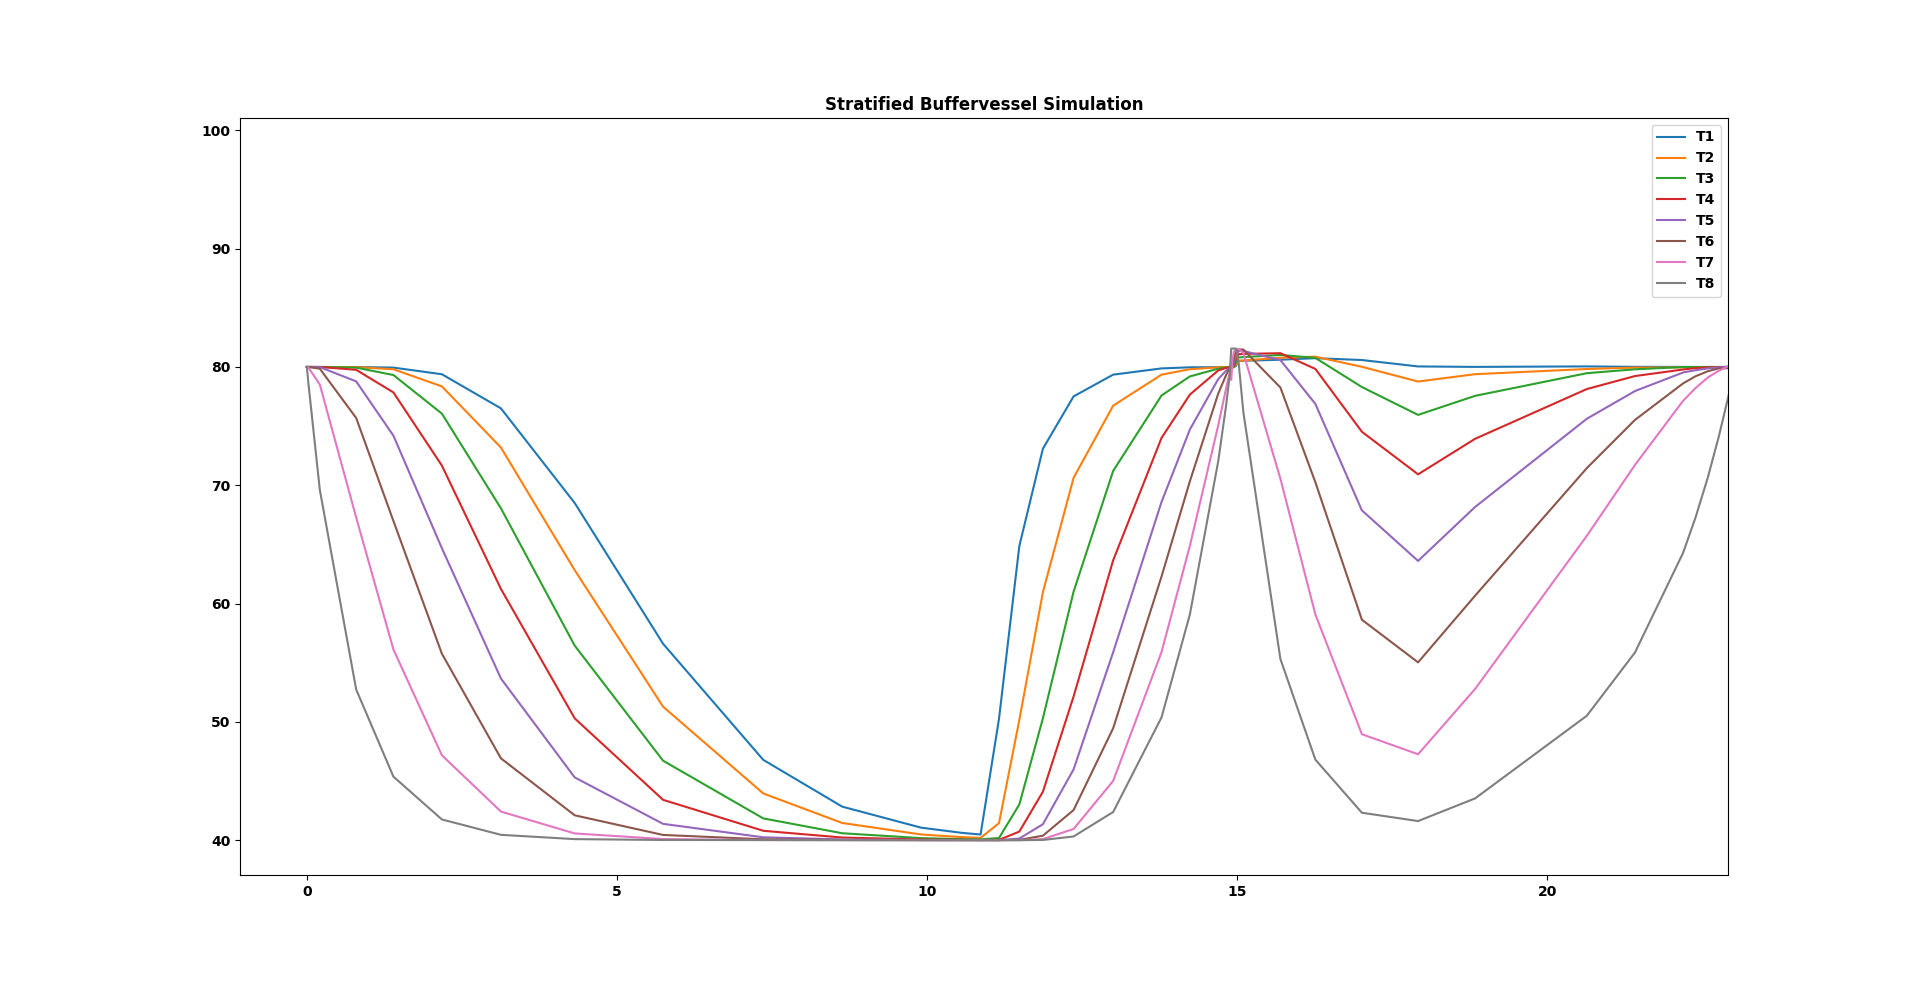
\includegraphics[width=0.8\columnwidth]{Figures/Python_validation_graph_buffervessel.png} }}
	\caption{Comparison between paper and python model}
	\label{fig:Comparison}
\end{figure}

\newpage
	\section{Change in Solver Report}

\subsection{Current situation}

In the orginal house.py file in the simulation folder, there is a function \textsf{scipy.integrate.odeint}  that calculates the ordinary differential equations from the domestic building model. The \textsf{SciPy} website states however that this function should be replaced with \textsf{scipy.integrate.solve\_ivp}. 

The code of the original ODE calculation in \textsf{house.py} is as follows:

\begin{lstlisting}
	
	for i in range(len(t)-1):
	
	err = SP_T[i+1] - Tair[i]
	Qinst = err * kp
	Qinst = np.clip(Qinst, 0, 7000)
	
	if (T_outdoor[i]>= 15):
	Qinst=0
	else:
	Qinst=Qinst
	
	inputs = (T_outdoor[i], Q_internal[i], Q_solar[i], SP_T[i], Qinst, CF,
	Rair_outdoor, Rair_wall, Cair, Cwall)
	# print(i)
	ts = [t[i], t[i+1]]
	y = odeint(model, y0, ts, args=inputs)
	
	Tair[i+1] = y[-1][0]
	Twall[i+1] = y[-1][1]
	# integral[i+1]         = y[-1][2]
	
	# Adjust initial condition for next loop
	
	y0 = y[-1]
\end{lstlisting}

The way the \textsf{odeint} function is used in the original file is not correct. It is used in a \textsf{for} loop, in which only 2 points in time are used as input to calculate the state, in this case $T_{air}$ and $T_{wall}$. The output state that is generated in the iteration of the loop, is then used as input for the next iteration. This causes unwanted oscillations in the output.

Control of the heat source $\dot{Q}_{inst}$ to control the indoor air temperature is also included in the \textit{for} loop, however, it would be more beneficial to have the control part of the model inside the house model itself.

\subsection{Changes needed in the code to switch solver}

The routine can be improved by using the \textsf{solve\_ivp} function from the \textsf{SciPy} library and removing the \textsf{for} loop.

The function has similar arguments, however, in the \textsf{solve.ivp} function, the input variables \textsf{y0} and time data \textsf{t} are switched (see below).


\begin{lstlisting}
	#odeint example
	y = odeint(model, y0, ts, args=inputs)
	#solveivp example
	y = solve_ivp(model_buffervessel, [0, t[-1]], y0, args=inputs)
\end{lstlisting}

The inputs in the \textsf{odeint} function are single values. However, for the \textsf{solve\_ivp} function an array is used for the inputs, since the inputs can change over time. An example is the setpoint of the indoor temperature. In the original file, the inputs changed with the help of the for loop, but the for loop will be removed with the \textsf{solve\_ivp} function.

By incorporating the changes, the code snippet from the original file (see top of this document) can be replaced with the snippet below.

\begin{lstlisting}
	inputs = (T_outdoor, Q_internal, Q_solar, SP_T, CF,
	Rair_outdoor, Rair_wall, Cair, Cwall, UAradiator, Crad, Cbuffervessel, cpwater)
	y = solve_ivp(model_buffervessel, [0, t[-1]], y0, args=inputs)
\end{lstlisting}

\subsection{Result of comparison between the solvers}

Incorporating these changes will result in the following difference:

\begin{figure}[ht]
	\centering
	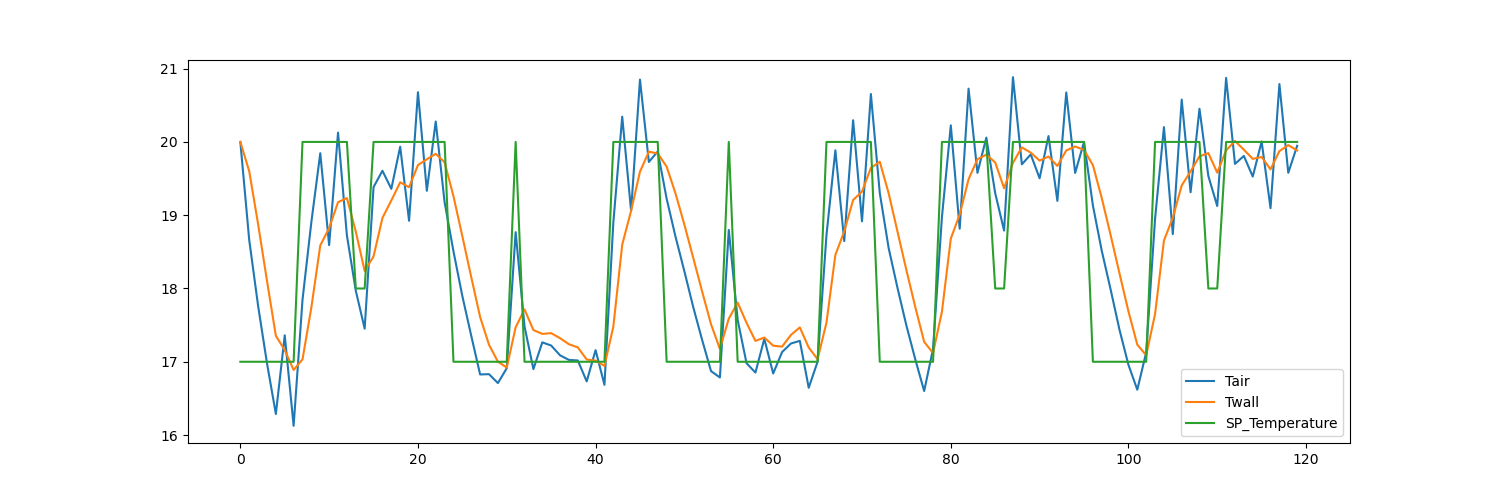
\includegraphics[width=1\columnwidth]{Figures/odeint_with_for_loop.png}
	\caption[Short title]{Indoor (wall)temperature output with \textsf{odeint}}
	\label{fig:profilelabels}
\end{figure}

\begin{figure}[ht]
	\centering
	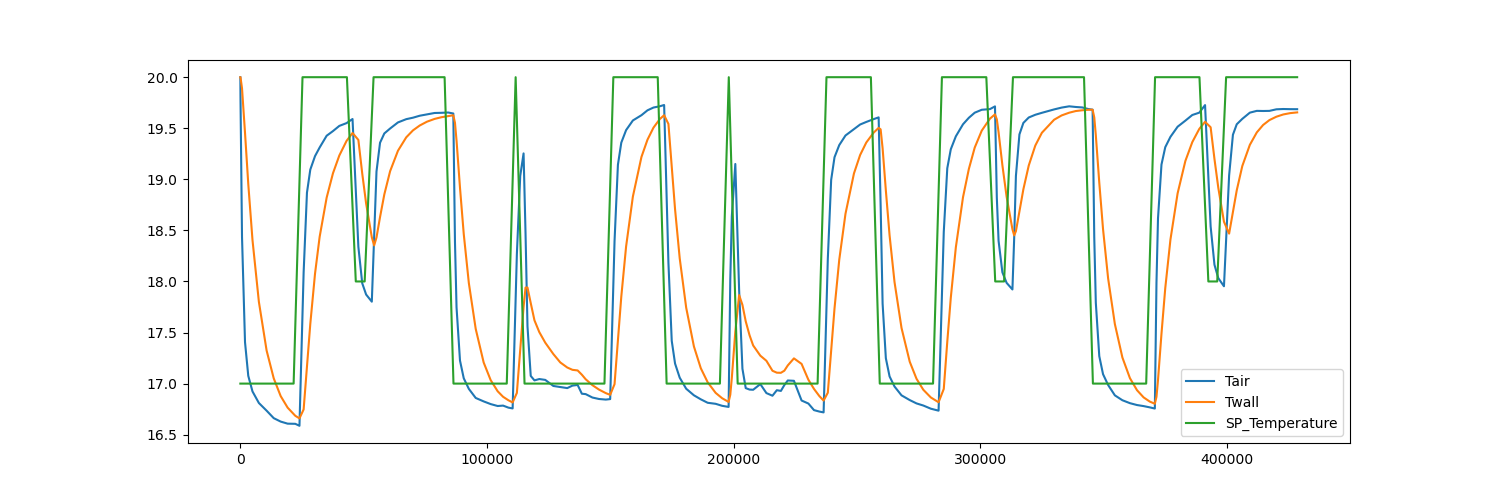
\includegraphics[width=1\columnwidth]{Figures/solve_ivp_without_for_loop.png}
	\caption[Short title]{Indoor (wall)temperature output with \textsf{solve\_ivp}}
	\label{fig:profilelabels}
\end{figure}

As can be seen, a much smoother output is created by using the \textsf{solve\_ivp} function.








\newpage
	\chapter{2 Zones house model 7R4C network}

The 4R-7C house model structure is implemented as described below:
	
\begin{figure}[H]
	\centering
	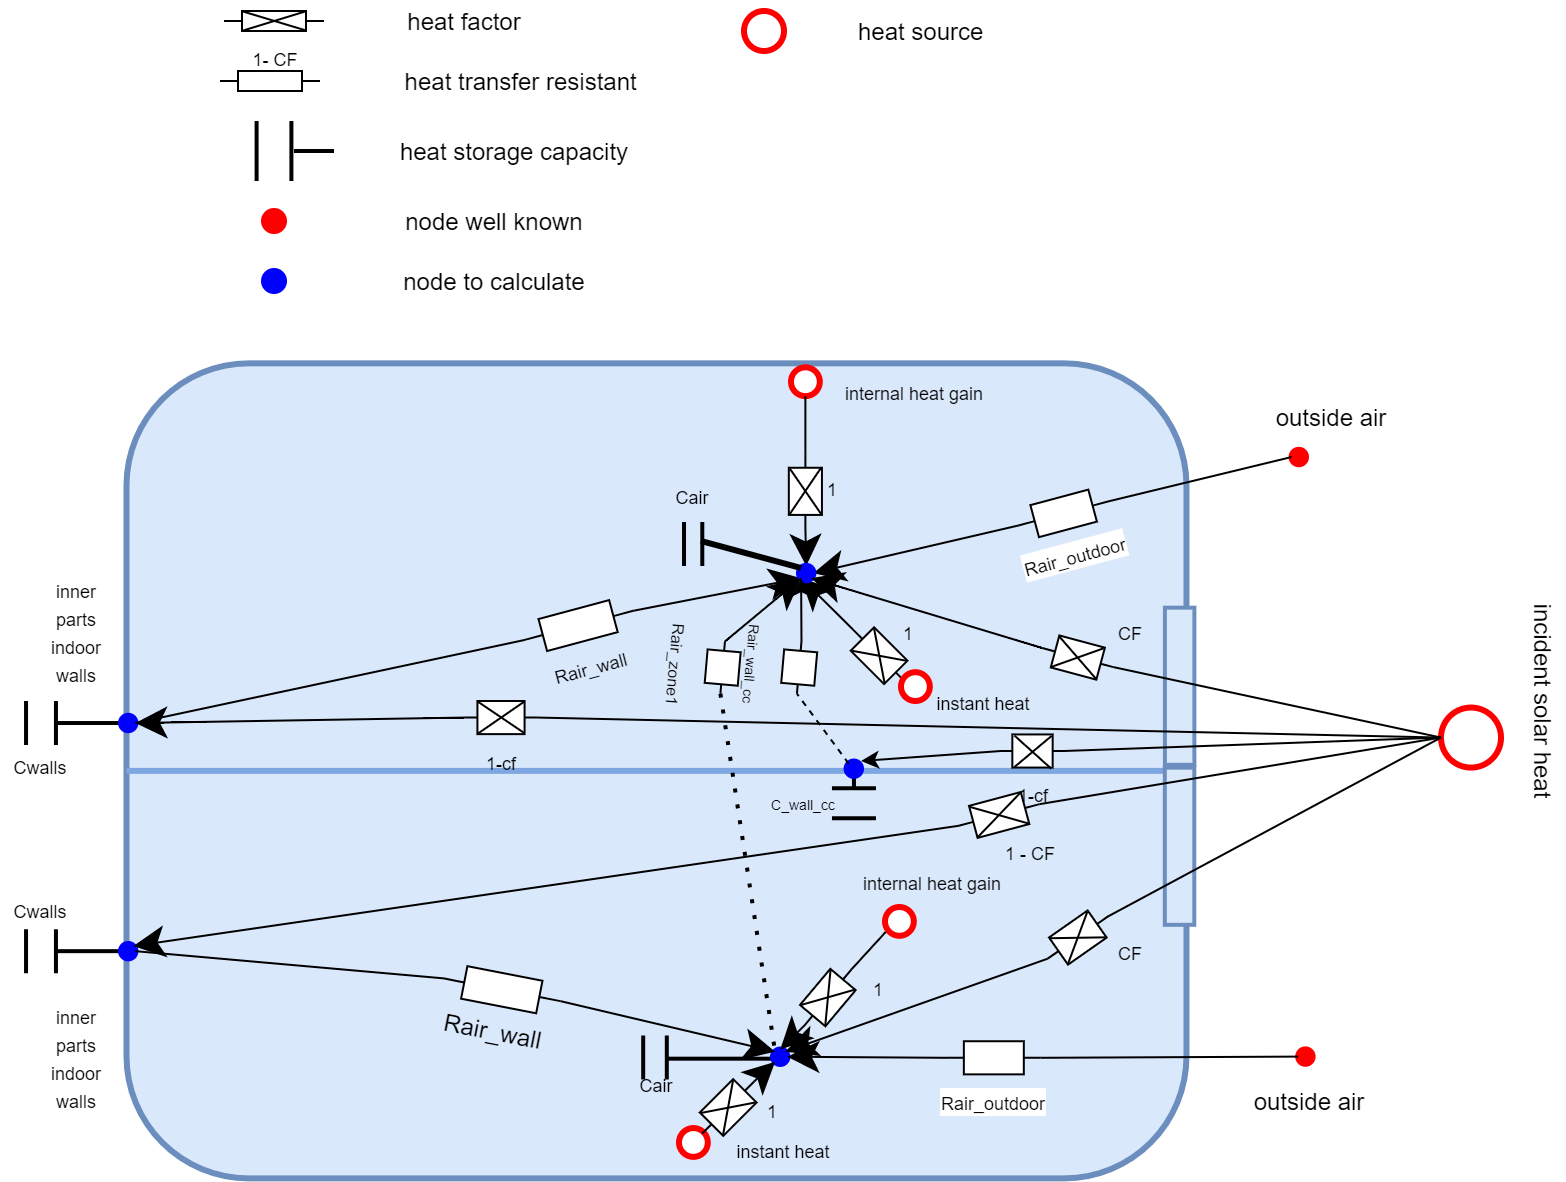
\includegraphics[width=1.0\columnwidth]{Pictures/House_electrical_circuits overview.png}
	\caption[Short title]{Schematic of a 2 zones house model}
	\label{fig:schema7R4C}
	\end{figure} 
	
The equivalent electrical 7R-4C network with components and topology is given in Fig. \ref{fig:elec7R4C}.

\begin{figure}[H]
	\centering
	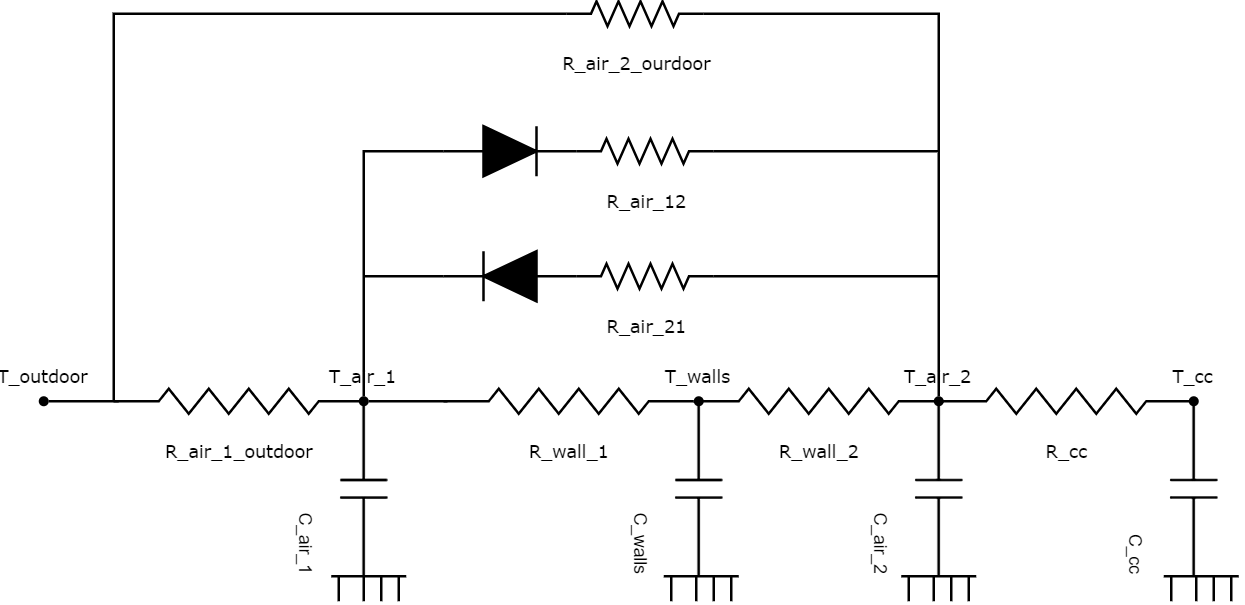
\includegraphics[width=1.0\columnwidth]{Pictures/2_Zones_house_circuits.png}
	\caption[Short title]{R-C circuits of 2 zones house model}
	\label{fig:elec7R4C}
	\end{figure}

with:\\
\begin{itemize}
    \item \texttt{T\_outdoor} : outdoor temperature [$\degr C$] 
    \item \texttt{T\_air\_1}  : zone 1 air temperature [$\degr C$]
    \item \texttt{T\_walls}   : wall temperature [$\degr C$]
    \item \texttt{T\_air\_2}  : zone 2 air temperature [$\degr C$]
    \item \texttt{T\_cc}      : temperature of the concrete layer between zone 1 and zone 2 [$\degr C$]
    \item \texttt{R\_air\_1\_outdoor} : outdoor resistance valus.
    \item \texttt{R\_wall\_1} : walls resistance value.
    \item \texttt{R\_wall\_2} : walls resistance value.
    \item \texttt{R\_cc}      : concrete resistance value.
    \item \texttt{R\_air\_12} : resistance value of air flow from zone 1 to zone 2.
    \item \texttt{R\_air\_21} : resistance value of air flow from zone 2 to zone 1.

\end{itemize}
\newpage
	\section{PID Controller}

\subsection{Introduction}

The report give an overview and compare between the available PID and advance python control packages. The different PID forms will be discussed in section 2. In section 3 and 4 are the most used PID Python packages in practice with their advantages and disadvantages. Finally section 5 give an overview on some advance control and optimization python library.

\subsection{The PID Forms}

The PID controller are available on 3 main different form: Interactive, Non interactive (“standard”, “mixed” or sometimes “ideal) and Parallel.  

\textbf{The series form} sometime also call classical, real or interactive in equation (1) is the oldest controller used for direct field control which is either both of its input (PV) and output (MV) are directly connected to field or process equipment \cite{Wolfgang}. The original pneumatic and electronic controllers had this algorithm, and it is still found in many digital PID controllers today. The controller has been programmed to implement the interacting PID equation even though it is no longer an artifact of the hardware. The rationale for this programming is to have the digital controller behave identically to the legacy analog electronic or pneumatic controller it is replacing. This way, the proven tuning parameters of the old controller may be plugged into the new digital controller, yielding the same results.  
The famous Ziegler-Nichols PID tuning method was developed for this controller algorithm. 

\begin{figure}[H]
	\centering
	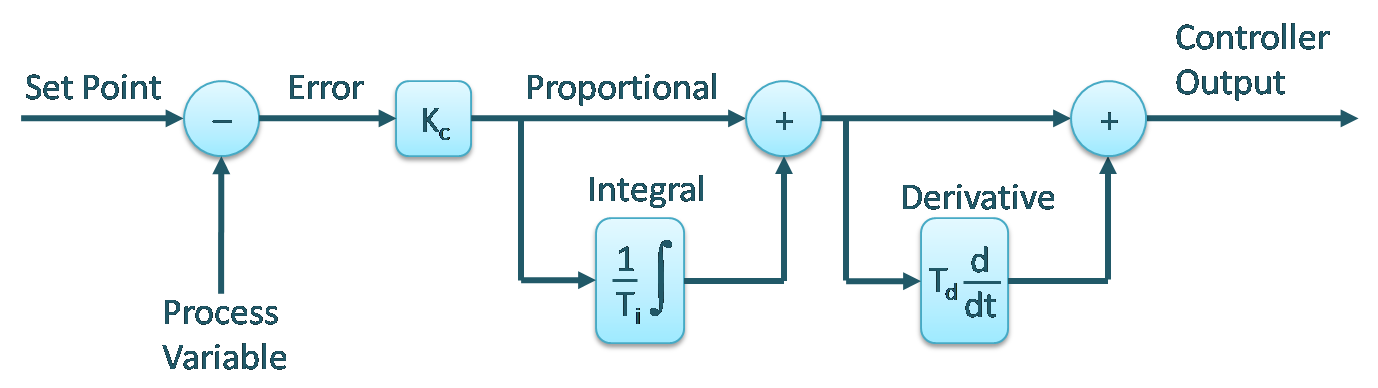
\includegraphics[width=0.8\columnwidth]{Figures/series.png}
	\caption[Short title]{Serial form PID Controller \cite{PID}}
	\label{figure: Serial PID}
\end{figure}

\begin{equation}
	\label{eqn:1}
	CO = K_c\cdot\left(e + \frac{1}{T_i}\int e\cdot dt \right)\cdot \left(1 + T_d\frac{de}{dt} \right)
\end{equation}


% A third version, with origins in the peculiarities of pneumatic controller mechanisms and analog electronic circuits, is called the Series or Interacting equation: 

% This “interacting” equation is an artifact of certain pneumatic and electronic controller designs. p Back when these were the dominant technologies, and PID controllers were modular designed such that integral and derivative actions were separate hardware modules included in a controller at additional cost beyond proportional-only action, the easiest way to implement the integral and derivative actions was in a way that just happened to have an interactive effect on controller gain. In other words, this odd equation form was a sort of compromise made for the purpose of simplifying the physical design of the controller. 

\textbf{The Ideal form} or non interactive algorithm is also called the standard or ISA algorithm. This form of controller is the classical teaching model of PID algorithms. It gives a clear understanding of P, I and D control, since: P-control, I-control and D-control can be seen independently of each other. Then, PID is effectively a combination of independent P, I and D-control actions. This can be seen in figure \ref{figure: Ideal PID} and euqation (2).
Since P, I and D algorithms are calculated independently in an ideal PID-controller. The Cohen-Coon and Lambda PID tuning rules were designed for this algorithm

\begin{figure}[H]
	\centering
	\includegraphics[width=0.8\columnwidth]{Figures/ideal.png}
	\caption[Short title]{Ideal form PID Controller \cite{PID}}
	\label{figure: Ideal PID}
\end{figure}

\begin{equation}
	\label{eqn:2}
	CO = K_c\cdot\left(e + \frac{1}{T_i}\int e\cdot dt +T_d\frac{de}{dt} \right)
\end{equation}

% An ideal process variable is a noise-free, refined and optimized variable. They are a result
% of computer optimization, process modeling, statistical filtering and value prediction
% algorithms

Note: If no derivative is used (i.e. Td = 0), the interactive and non interactive controller algorithms are identical. 

\textbf{The parallel form} has not often discussed in academic textbooks, but it is widely used nowadays in the  industry sector (distributes control system (DCSs) and PLCs application). This algorithm is simple to understand, but more difficult to tune. It has no controller gain affecting all three control modes (3 controller-action need to be tune separately), as a result it take more time to get the correct controller parameters. 

% Adjusting the proportional gain should be supplemented by adjusting the integral and derivative settings at the same time.

\begin{figure}[H]
	\centering
	\includegraphics[width=0.8\columnwidth]{Figures/parallel.png}
	\caption[Short title]{Parallel form PID Controller \cite{PID}}
	\label{figure: Parallel PID}
\end{figure}

\begin{equation}
	\label{eqn:3}
	CO = K_p\cdot e + K_i\int e\cdot dt +K_d\cdot\frac{de}{dt}
\end{equation}

\textbf{Significance of Different Algorithms }

The biggest difference between the controller algorithms is that the parallel controller has a true proportional gain ($K_p$), while the other two algorithms have a controller Gain ($K_c$). The  $K_c$ Gain affects all three modes (Proportional, Integral and Derivative) of the Series and Ideal controllers, while $K_p$  affects only the proportional mode of a Parallel controller. 

This difference has a major impact on the tuning of the controllers. All the popular tuning rules (Ziegler-Nichols, Cohen-Coon, Lambda, and others) assume the controller does not have a parallel structure. 

% To tune a Parallel controller using any of these rules, the Integral time has to be divided and derivative time multiplied by the calculated Controller Gain. 

The second difference between the controller algorithms is the interaction between the \textbf{Integral} and \textbf{Derivative} modes of the Series (Interactive) controller. This is only of significance if the Derivative mode is used. In most PID controller applications, Derivative mode is not used  In practice D-action is not often used because of its sensitivity to the sensor noise. 

% Beyond the differences mentioned above, controllers also differ in the way the changes on controller output is calculated (positional and velocity algorithms), in the way Proportional and Derivative modes act on set point changes, in the way the Derivative mode is limited/filtered, as well as a interesting array of other minor differences. These differences are normally subtle, and should not affect your tuning. 

% To cut a long story short, it is hard to prescribe a particular form to implement a PID controller, each has its drawbacks and advantages. The standard structure is the most widespread in the field of industry. 
In the end, when tuning the controller, it is important to know what structure of the controller is (There are formulas to switch from one to another).

\subsection{PID in practice.}

% Implement PID in practice
The Ideal and parallel PID in equation (1) and (2) can be easily converted from one to another with  $K_i = \frac{Kc}{T_i}$ and $K_d = \frac{Kc}{T_d}$.

Let Consider the independent PID equation (parallel):
\begin{equation}
	\label{eqn:4}
	CO = K_p\cdot e + K_i\int e\cdot dt +K_d\cdot\frac{de}{dt}
\end{equation}

Where CO is the controller output, e=SP-PV, SP is the setpoint, PV the process variable (system output). Differentiating both sides of [4] gives:

\begin{equation}
	\label{eqn:5}
	dCO = K_p\cdot de + K_i\cdot e \cdot dt + K_d\frac{d(de)}{dt}
\end{equation}

Using difference to approximate the differential we get discrete PID equation.

\begin{equation}
	\label{eqn:6}
	CO(t) = CO(t-1) + K_p[e(t) - e(t-1)] + K_i\cdot T \cdot e(t) + \frac{K_d}{T}[e(t) - 2e(t)-1) + e(t-2)]
\end{equation}

Where T is the sampling period. The D-term of this equation contains set point and changes in set point may cause an unwanted change in CO (a Dirac function \cite{Delta_Function}, some time call derivative Kick ). Remove set point from D-term we get equation [6] (e = SP - PV, de = dSP -dPV, when SP is constant de = dPV).

\begin{equation}
	\label{eqn:7}
	CO(t) = CO(t-1) + K_p[e(t) - e(t-1)] + K_i\cdot T \cdot e(t) + \frac{K_d}{T}[PV(t) - 2PV(t)-1) + PV(t-2)]
\end{equation}

Many industrial PID controllers use equation [6] (e.g. Allen Bradley PLCs). However, if we remove set point from both P-term and D-term, we get a still better PID equation [7].

\begin{equation}
	\label{eqn:8}
	CO(t) = CO(t-1) + K_p[PV(t) - PV(t-1)] + K_i\cdot T \cdot e(t) + \frac{K_d}{T}[PV(t) - 2PV(t)-1) + PV(t-2)]
\end{equation}

To implement PID controller in practice a few more things need to be addressed.

\begin{itemize}
	\item Windup protection.
	\item On the fly tuning: a good PID controller allow changing the parameters when the process is running.
	\item Online Controller Switching or bumpless transfer:  allow smooth transition from one type of controller to another (ex: switch from PID to manual control, or MPC).
	\item 2 DOF (degree of freedom) PID (Optional) 
\end{itemize}

A good explanation on the practical problems and solution can be found in the the blog series improving the Beginner’s PID by Brettbeauregard \cite{Improving_PID}.

\subsection{The PID Python Libraries}

Most of PID python libraries had been developed base on the Arduino PID and series blog by Beauregard \cite{Arduino_PID}  \cite{Improving_PID}. The Arduino version has been updated by 
Gelraen \cite{Arduino_PID_V2} on January 2021.

\subsubsection{Python packages.}
% \textbf{}
This subsection will give a quick overview on the most use python packages.

\textbf{Simple PID} \cite{Simple_Pid} follow the guideline implementation by Brett Beauregard  \cite{Improving_PID}. The package has included the windup protection, the derivative kick avoidance, online parameters tuning, smooth controller transition from Auto (PID on) to manual. The last update was on 17 November 2020

\textbf{ivPID} \cite{ivPID} PID controller implementation base on equation [\ref{eqn:4}] with windup protection. This package does not has derivative kick avoidance or smooth controller switching.

\textbf{DvG${\_}$PID${\_}$Controller} \cite{DvG_PID_Controller}: another Arduino library \cite{Arduino_PID} ported to Python by Dennis van Gils (a senior research of Twente University) in july 2020. This package has include all functionality from Arduino library ( windup protection, derivative kick, controller switch, bumpless transfer).

\subsubsection{PID design example with Jupiter notebook}

There are many other PID controller example had been written in python. A few more example are mentioned below:

An explanation on PID controller and python implementation can be found in \href{https://apmonitor.com/pdc/index.php/Main/ProportionalIntegralDerivative}{apmonitor dynamic and control website}.

\begin{figure}[H]
	\centering
	\includegraphics[width=0.8\columnwidth]{Figures/PID_interactive.png}
	\caption[Short title]{Pid interactive notebook on apmonitor}
	\label{figure:interactive notebook}
\end{figure}

\newpage

A Jupyter/Python notebooks series on PID controller on (chapter 4) chemical process course of Notre Dame University\cite{CBE}.

\begin{figure}[H]
	\centering
	\includegraphics[width=0.8\columnwidth]{Figures/PID_NotreDame.png}
	\caption[Short title]{Pid controller notebook series of Notre Dame University chemical process course.}
	\label{figure:NotreDame notebook}
\end{figure}

\subsection{Python control system packages.}

In this chapter some advance python control and optimization packages will be discussed.

The first one is \textbf{python Control Systems} Library v0.84 \cite{Control_Lib} \cite{GitControl_Lib} with the last update on 16/03/2021 (the day when this report is written).

The main features are: 

\begin{itemize}
	\item Linear input/output systems in state-space and frequency domain
	
	\item Nonlinear input/output system modeling, simulation, and analysis
	
	\item Block diagram algebra: serial, parallel, and feedback interconnections
	
	\item Time response: initial, step, impulse
	
	\item Frequency response: Bode and Nyquist plots
	
	\item Control analysis: stability, reachability, observability, stability margins
	
	\item Control design: eigenvalue placement, LQR, H2, Hinf, MPC
	
	\item Model reduction: balanced realizations, Hankel singular values
	
	\item Estimator design: linear quadratic estimator (Kalman filter)
	
	\item The optimal control module with optimization based controllers for nonlinear systems with state and input constraints.
	
\end{itemize}

Another python package for machine learning and optimization is \textbf{GEKKO Optimization Suite}\cite{gekko2018}. It is coupled with large-scale solvers for linear, quadratic, nonlinear, and mixed integer programming (LP, QP, NLP, MILP, MINLP). Modes of operation include parameter regression, data reconciliation, real-time optimization, dynamic simulation, and nonlinear predictive control. The paper release with the package has been selected as a 2020 Best Paper by the journal Processes (figure: \ref{figure:Gekko}). 

\begin{figure}[H]
	\centering
	\includegraphics[width=0.8\columnwidth]{Figures/gekko_best_paper2020.png}
	\caption[Short title]{Gekko best paper award 2020}
	\label{figure:Gekko}
\end{figure}

Beside the 2 python packages which have been mentioned above there is a collection of Jupiter python/notebook series on optimization and control CBE 30338 (figure \ref{figure:CBE}) and CBE 32338 (\ref{figure:CBE_Lab}) Chemical Process Control \cite{CBE} \cite{CBE_Lab}. The notebooks series contain a lot of python example on optimization technique. For example, the linear programming has been mentioned in section 6.3 \cite{CBE} CBE 30338 (\ref{figure:CBE}) and the model predictive control in section 5.1, 5.2 \cite{CBE_Lab} CBE 32338 (\ref{figure:CBE_Lab}) 

\begin{figure}[H]
	\centering
	\includegraphics[width=0.8\columnwidth]{Figures/Optimization_CBE.png}
	\caption[Short title]{CBE 30338 Chemical Process Control}
	\label{figure:CBE}
\end{figure}

\begin{figure}[H]
	\centering
	\includegraphics[width=0.8\columnwidth]{Figures/Optimization_CBE_Lab.png}
	\caption[Short title]{CBE 32338 Process Control Laboratory}
	\label{figure:CBE_Lab}
\end{figure}

\newpage


	\section{Finite-element discretization}

\subsection{Heat pump discretization}

Het algemene model van de warmtepomp en airco wordt afgeleid met behulp van het volgende geschematiseerde black box model:

\subsection{Buffer vessel discretization}

Als voorbeeld van een model met warmtestromen en warmtediffusie wordt het volgende model van
een buffervat beschouwd:

\begin{figure}[H]
	\centering
	\includegraphics[width=0.7\columnwidth]{Pictures/FEwatervat.png}
	\caption[Short title]{Finite-element buffer vessel}
	\label{fig:FEbuffervessel}
\end{figure}

Dit is een buffervat in een verwarmingsinstallatie.

Voor het modelleren hiervan wordt gebruik gemaakt van een tweetal universele elementen:

\begin{enumerate}
	\item Exchange element. Dit element beschrijft warmtetransportt via een vloeistofstroom $F$ door het element en warmtetransport door geleiding. Het element kan een warmtecapaciteit
	hebben.
	\item Een puntbron. Deze bron beschrijft warmteontwikkeling of warmte-onttrekking in een punt.
\end{enumerate}

Het vat is verdeeld in 3 niveaus over de hoogte:
\begin{enumerate}
	\item Bovenzijde vat (element 3)
	\item Midden vat( element 4 )
	\item Onderzijde vat (element 5 )
\end{enumerate}

In het vat is sprake van:
\begin{itemize}
	\item Warmteverlies naar andere temperatuurniveau ’s en naar de omgeving. De
	omgevingstemperatuur in dit model is gegeven door de temperatuur in punt 7.
	De elementen die het volume van het vat beschrijven (E3,E4 en E5) wisselen warmte uit naar
	elkaar en naar punt 6.
	\item Warmtetransport door waterstromen. In waterstromen buiten het vat wordt warmte
	onttrokken of toegevoegd. In het vat is een waterstroom die zorgt voor het kortsluiten van
	de kringlopen.
\end{itemize}

Deze beide mechanismen worden meegenomen in het model.

Er wordt verondersteld dat gebruik wordt gemaakt van gelaagdheid. Boven in het vat heerst een
hogere temperatuur dan onderin het vat. Daarnaast is er sprake van een tweetal leidingen waarin
warmte wordt uitgewisseld met de omgeving:

\begin{itemize}
	\item Een leiding waarin warmte wordt toegevoegd aan het vat $\dot{Q}_{add}$. Deze leiding neemt
	vloeistof (water) onder uit het vat (punt 5), verhoogt de temperatuur door warmte-inbreng
	(punt 1) en brengt het water boven in het vat weer in. Deze leiding bestaat uit de
	elementen E1 (boven) en E2 (onder). In deze leiding is een vloeistofstroom $F_1 (kJ/(K·s))$
	aanwezig die de warmte transporteert.
	\item Een leiding waarin warmte wordt onttrokken aan het vat $\dot{Q}_{use}$. Deze leiding neemt vloeistof (water) boven uit het vat (punt 2), verlaagt de temperatuur door warmteonttrekking (punt 7) en brengt het water boven in het vat weer in. Deze leiding bestaat uit	de elementen E10 (boven) en E11 (onder). In deze leiding is een vloeistofstroom $F_2 (kJ/(K·s))$ aanwezig die de warmte transporteert.
\end{itemize}

\subsection{Matrixvergelijking}

Voor het oplossen van de temperatuurverdeling wordt per knooppunt een energiebalans opgesteld.
Deze energiebalans resulteert in een matrixvergelijking.

\begin{equation}
	\begin{aligned}
	    \mathbf{K \theta + C \dot{\theta}} = \mathbf{\dot{q}}	    	
	\end{aligned}
\end{equation}

$K$: de warmtegeleidingsmatrix (W/K)
$C$: de warmtecapaciteitsmatrix (J/K)
$\theta$: de temperatuursvector (K)
$\dot{\theta}$: de tijdsafgeleide van de temperatuursvector (K/s)
$\dot{q}$: de vector met thermische brontermen (W)

\subsection{Elementen in de stroming}

Om te komen tot het matrixmodel wordt begonnen met één exchange element zoals hierboven
geïntroduceerd (E1,E2,E3,E4,E5,E10,E11). Dit element bevat 2 knooppunten. De volgende veronderstellingen worden gedaan:

\begin{itemize}
	\item Het element bevat 2 knooppunten waarmee deze verbonden is met de omgeving. De
	nummering bedraagt: $n_1$ en $n_2$.
	\item Binnen het element heerst een lineair verlopende temperatuur, van knooppunt naar
	knooppunt.
	\item Binnen het element is een vloeistofstroom $F$ die zorgt voor additioneel warmtetransport. De stroomrichting is van knooppunt 1 naar knooppunt 2.
	\item De warmtecapaciteit van het element wordt evenredig verdeeld over de knooppunten.
\end{itemize}

De warmtestroom vanuit het element naar knoopunten 1 en 2 moet in balans zijn met de andere
warmtestromen en de warmtegeneratie in de betreffende knooppunten.

\begin{figure}[H]
	\centering
	\includegraphics[width=0.7\columnwidth]{Pictures/exchange_element.png}
	\caption[Short title]{Exchange element buffer vessel}
	\label{fig:exchange_element}
\end{figure}

Voor de warmtestromen vanaf knooppunt 1 geldt:

\begin{equation}
	\begin{aligned}
		(T_1 - T_2) \cdot \frac{1}{R_e} + C_{e1,1} \cdot \frac{dT_1}{dT} = \dot{Q}_{ext,1}	    	
	\end{aligned}
\end{equation}

$T_1$: temperatuur in knooppunt 1 \\
$T_2$: temperatuur in knooppunt 2 \\
$R_e$: warmteweerstand voor geleiding tussen knooppunt 1 en 2 \\
$C_{e1,1}$: warmtecapaciteit in knooppunt 1 van element 1 \\
$\frac{dT_1}{dT}$: temperatuursverandering in de tijd in knooppunt 1 \\
$\dot{Q}_{ext,1}$: externe warmtetoevoer in knooppunt 1 \\

De vloeistofstroom $F$ vanuit knooppunt $T_1$ heeft dezelfde temperatuur als $T_1$ en heeft dus geen invloed op de temperatuur in $T_1$.

Voor de warmtestromen vanaf punt 2 geldt:

\begin{equation}
	\begin{aligned}
		(T_2 - T_1) \cdot \frac{1}{R_e} + F \cdot (T_2 - T_1) + C_{e1,2} \cdot \frac{dT_2}{dT} = \dot{Q}_{ext,2}	    	
	\end{aligned}
\end{equation}

$C_{e1,2}$: warmtecapaciteit in knooppunt 2 van element 1 \\
$\frac{dT_2}{dT}$: temperatuursverandering in de tijd in knooppunt 2 \\
$\dot{Q}_{ext,2}$: externe warmtetoevoer in knooppunt 2 \\

In matrixnotatie:

\begin{equation}
	\begin{aligned}
	\begin{bmatrix}
	    1/R_e & -1/R_e \\
	    -1/R_e -F &  1/R_e + F
    \end{bmatrix}
    \cdot
    \begin{bmatrix}
    	T_1 \\
    	T_2
    \end{bmatrix}
    +
    	\begin{bmatrix}
    	C_{e1,1} & 0 \\
    	0 &  C_{e1,2}
    \end{bmatrix}
    \cdot
    \begin{bmatrix}
    	\frac{dT_1}{dt} \\
	    \frac{dT_2}{dt}
    \end{bmatrix}	
    =
        \begin{bmatrix}
    	\dot{Q}_{ext,1} \\
    	\dot{Q}_{ext,2}
    \end{bmatrix}  	
	\end{aligned}
\end{equation}

Merk op dat door de aanwezigheid van een vloeistofstroom $F$, de geleidingsmatrix niet langer symmetrisch is.

Daarnaast wordt gebruik gemaakt van elementen die alleen een warmteweerstand weergeven. Deze
elementen (E6,E7,E8 en E9) kunnen worden gerepresenteerd met de volgende matrixvergelijking

\begin{equation}
	\begin{aligned}
		\begin{bmatrix}
			1/R_e & -1/R_e \\
			-1/R_e &  1/R_e
		\end{bmatrix}
		\cdot
		\begin{bmatrix}
			T_1 \\
			T_2
		\end{bmatrix}	
		=
		\begin{bmatrix}
			\dot{Q}_{ext,1} \\
			\dot{Q}_{ext,2}
		\end{bmatrix}  	
	\end{aligned}
\end{equation}

\subsection{Systemmmatrices van het buffervat}

Er wordt nu een systeemmatrix opgesteld voor het schematisch weergegeven model. Deze
systeemmatrix wordt opgebouwd uit de verschillende elementmatrices. De noodzakelijke rang van
deze systeemmatrix is het aantal knooppunten in het warmtestroomschema minus het aantal
voorgeschreven knooppunten in dit schema. Er zijn 7 knooppunten in het model. In dit geval wordt
in punt 6 de temperatuur voorgeschreven.
Er resteren dan 6 onafhankelijke vrijheidsgraden.

\subsubsection{Capaciteitsmatrix $\mathbf{C}$}

There are 7 nodes in the system. The heat capacities are:

\begin{equation}
	\begin{aligned}
\text{node 1} & \quad C_{e1,1} + C_{e2,2} = 0.5 \cdot (C_{e1} + C_{e2})\\
\text{node 2} & \quad C_{e1,2} + C_{e3,1} + C_{e10,2} + C_{e6,2} = 0.5 \cdot (C_{e1} + C_{e3} + C_{e10} + C_{e6}) \\
\text{node 3} & \quad C_{e3,2} + C_{e4,1} + C_{e7,2} = 0.5 \cdot (C_{e3} + C_{e4} + C_{e7}) \\
\text{node 4} & \quad C_{e4,2} + C_{e5, 1} + C_{e8,2} = 0.5 \cdot (C_{e4} + C_{e5} + C_{e8}) \\
\text{node 5} & \quad C_{e5,2} + C_{e2, 1} + C_{e9, 2} + C_{11,2} = 0.5 \cdot (C_{e5} + C_{e2} + C_{e9} + C_{11}) \\
\text{node 6} & \quad C_{e6,1} + C_{e7, 1} +  C_{e8, 1} +  C_{e9, 1} = 0.5 \cdot (C_{e6} + C_{e7} +  C_{e8} +  C_{e9}) \\
\text{node 7} & \quad C_{e10,2} + C_{e11,1} = 0.5 \cdot (C_{e10} + C_{e11})
	\end{aligned}
\end{equation}

\begin{tiny}
\[
0.5 \cdot 
\begin{bmatrix}
	C_{e1} + C_{e2} & 0 & 0 & 0 & 0 & 0 & 0 \\
	0 & C_{e1} + C_{e3} + C_{e10} + C_{e6} & 0 & 0 & 0 & 0 & 0 \\
	0 & 0 & C_{e3} + C_{e4} + C_{e7} & 0 & 0 & 0 & 0 \\
	0 & 0 & 0 & C_{e4} + C_{e5} + C_{e8} & 0 & 0 & 0 \\
	0 & 0 & 0 & 0 & C_{e5} + C_{e2} + C_{e9} + C_{e11} & 0 & 0 \\
	0 & 0 & 0 & 0 & 0 & C_{e6} + C_{e7} +  C_{e8} + C_{e9} & 0 \\
	0 & 0 & 0 & 0 & 0 & 0 & C_{e10} + C_{e11}
\end{bmatrix}
\]
\end{tiny}

The heat capacities of element E1, E2, E10 and E11 (pipelines) are very small and can be approximated to be zero. Also, the elements E6, E7, E8 and E9 are thermal leaks, connected to node 6, which may be a boundary condition.

The capacity matrix thus reduces to:

\[
0.5 \cdot 
\begin{bmatrix}
	\approx 0 & 0 & 0 & 0 & 0 & 0 & 0 \\
	0 & C_{e3} & 0 & 0 & 0 & 0 & 0 \\
	0 & 0 & C_{e3} + C_{e4} & 0 & 0 & 0 & 0 \\
	0 & 0 & 0 & C_{e4} + C_{e5} & 0 & 0 & 0 \\
	0 & 0 & 0 & 0 & C_{e5} & 0 & 0 \\
	0 & 0 & 0 & 0 & 0 & 0 & 0 \\
	0 & 0 & 0 & 0 & 0 & 0 & \approx 0
\end{bmatrix}
\]

In the approximation above, the buffer vessel system is not solvable, without adding some heat capacity to nodes N1 and N7. \emph{e.g.} these nodes must be coupled with a house model element with finite heat capacity.

In any case, the node N6 (boundary condition) does not contribute a DOF to the system of equations. Row 6 and column 6 will be removed from the set of equations.

\subsubsection{$\mathbf{\dot{q}}$-vector}

De vector $\mathbf{\dot{q}}$ wordt gegeven door:

\[
\left(\hspace{-5pt}\begin{array}{cc|c}
	1 & 1 & \dot{q}_1 = \dot{Q}_{add}\\
	2 & 2 & \dot{q}_2\\
	3 & 3 & \dot{q}_3\\
	4 & 4 & \dot{q}_4\\
	5 & 5 & \dot{q}_5\\
	6 & 6 & \dot{q}_6\\
	7 & 7 & \dot{q}_7 = -\dot{Q}_{use}
\end{array}\hspace{-5pt}\right)
\]

\[
\left(\hspace{-5pt}\begin{array}{cc|c}
	1 & 2 & 3 \\
	4 & 5 & 9
\end{array}\hspace{-5pt}\right)
\]

In nodes N1 and N7 an external een heat source / heat sink is contributing to the power balance.

Het voorgeschreven knooppunt (randvoorwaarde, boundary condition) 6 is verbonden aan knooppunten 2, 3, 4 en 5. Dit zijn de ook de vrijheidsgraden 2, 3, 4 en 5. Vrijheidsgraden worden aangegeven met DOF (degree of freedom). In de overeenkomstige knooppunten wordt de capaciteits? stiffness matrix $\mathbf{K}$ en de bronvector (load vector) $\mathbf{\dot{q}}$ aangepast.De aanpassing van de K-matrix wordt verderop toegelicht. De bronvector wordt als volgt aangepast:

\[
\begin{bmatrix}
	1 & 1 & \dot{Q}_{add} \\
	2 & 2 & 0 - \frac{1}{R_{2,6}} \\
	3 & 3 & 0 - \frac{1}{R_{3,6}} \\
	4 & 4 & 0 - \frac{1}{R_{4,6}} \\
	5 & 5 & 0 - \frac{1}{R_{5,6}} \\
	6 & 7 & -\dot{Q}_{use}
\end{bmatrix}
\]


\subsubsection{Geleidingsmatrix $\mathbf{K}$}

elements with heat capacity must have two nodes:
E3, E4, E5

elements without heat capacity have two nodes as well:
E1, E2, E6, E7, E8, E9, E10, E11

elements without heat conduction:
E1, E2, E10, E11

elements with heat conduction:
E3, E4, E5, E6, E7, E8, E9

elements with heat convection (flow):
E1, E2, E3, E4, E5, E10, E11

The "conduction" matrix is equivalent to the stiffness matrix in a mechanical FE analysis.
In terms of the thermal system topology this matrix contains the "edges" between the nodes. The matrix is setup as a 7 x 7 square zero matrix with the nodes as DOF.

\begin{equation}
	\begin{aligned}
		\begin{bmatrix}
			0 & 0 & 0 & 0 & 0 & 0 & 0\\
			0 & 0 & 0 & 0 & 0 & 0 & 0\\
			0 & 0 & 0 & 0 & 0 & 0 & 0\\
			0 & 0 & 0 & 0 & 0 & 0 & 0\\
			0 & 0 & 0 & 0 & 0 & 0 & 0\\
			0 & 0 & 0 & 0 & 0 & 0 & 0\\
			0 & 0 & 0 & 0 & 0 & 0 & 0\\
		\end{bmatrix}
	\end{aligned}
\end{equation}

The conductive elements in the system are:

\begin{equation}
	\begin{aligned}
        \frac{1}{R_{2,3}} & = & \frac{1}{R_{e3}} \\
        \frac{1}{R_{3,4}} & = & \frac{1}{R_{e4}} \\
        \frac{1}{R_{4,5}} & = & \frac{1}{R_{e5}} \\
        \frac{1}{R_{2,6}} & & \frac{1}{R_{3,6}} & & \frac{1}{R_{4,6}} & & \frac{1}{R_{5,6}} 
	\end{aligned}
\end{equation}

The conductive element $\frac{1}{R_{12}} = \frac{1}{R_{e1}} = 0$. This means $R_{12} \rightarrow \infty$. We assume, the pipeline is perfectly insulated and creates no heat leak. Thermal energy flowing \emph{through} it is completely delivered to the target node. Likewise, this holds for the elements E2, E10 and E11.

\begin{equation}
	\begin{aligned}
		\begin{bmatrix}
			0 & 0 & 0 & 0 & 0 & 0 & 0\\
            0 & 0 & \frac{-1}{R_{2,3}} & 0 & 0 & \frac{-1}{R_{2,6}} & 0 \\
            0 & \frac{-1}{R_{2,3}} & 0 & \frac{-1}{R_{3,4}} & 0 & \frac{-1}{R_{3,6}} & 0\\
            0 & 0 & \frac{-1}{R_{3,4}} & 0 & \frac{-1}{R_{4,5}} & \frac{-1}{R_{4,6}} & 0\\
            0 & 0 & 0 & \frac{-1}{R_{4,5}} & 0 & \frac{-1}{R_{5,6}} & 0 \\
            0 & \frac{-1}{R_{2,6}} & \frac{-1}{R_{3,6}} & \frac{-1}{R_{4,6}} & \frac{-1}{R_{5,6}} & 0 & 0\\
            0 & 0 & 0 & 0 & 0 & 0 & 0\\
		\end{bmatrix}
	\end{aligned}
\end{equation}

\begin{equation}
	\begin{aligned}
		\begin{bmatrix}
			0 & 0 & 0 & 0 & 0 & 0 & 0 \\
			0 & \frac{1}{R_{2,3}} + \frac{1}{R_{2,6}} & \frac{-1}{R_{2,3}} & 0 & 0 & \frac{-1}{R_{2,6}} & 0 \\
			0 & \frac{-1}{R_{2,3}} & \frac{1}{R_{2,3}} + \frac{1}{R_{3,4}} + \frac{1}{R_{3,6}} & \frac{-1}{R_{3,4}} & 0 & \frac{-1}{R_{3,6}} & 0 \\
			0 & 0 & \frac{-1}{R_{3,4}} & \frac{1}{R_{3,4}} +  \frac{1}{R_{4,5}} + \frac{1}{R_{4,6}} & \frac{-1}{R_{4,5}} & \frac{-1}{R_{4,6}} & 0\\
			0 & 0 & 0 & \frac{-1}{R_{4,5}} & \frac{1}{R_{4,5}} + \frac{1}{R_{5,6}} & \frac{-1}{R_{5,6}} & 0 \\
			0 & \frac{-1}{R_{2,6}} & \frac{-1}{R_{3,6}} & \frac{-1}{R_{4,6}} & \frac{-1}{R_{5,6}} & \frac{1}{R_{2,6}} + \frac{1}{R_{3,6}} +  \frac{1}{R_{4,6}} + \frac{1}{R_{5,6}} & 0\\
			0 & 0 & 0 & 0 & 0 & 0 & 0\\
		\end{bmatrix}
	\end{aligned}
\end{equation}

If node N6 is a boundary condition \emph{i.e.} $T_6$ is given as a constant. The corresponding row in the $\mathbf{K}$ and $\mathbf{C}$ matrices can be removed. For the nodes that are connected to node N6 (row 2, 3, 4 and 5) the thermal connection can be moved to the $\mathbf{\dot{q}}$ vector. This can be seen by writing down the differential equation for node N2:

\begin{equation}
	\begin{aligned}
        0.5 \, C_{e3} \cdot \frac{dT_2}{dt} = \frac{1}{R_{2,3}} (T_3 - T_2) + \frac{1}{R_{2,6}} (T_6 - T_2) & = (-\frac{1}{R_{2,3}} - \frac{1}{R_{2,6}}) \cdot T_2 + \frac{1}{R_{2,3}} \cdot T_3 + \frac{1}{R_{2,6}} \cdot T_6 
	\end{aligned}
\end{equation}

\begin{equation}
	\begin{aligned}
        \mathbf{K \theta} \qquad & + & \mathbf{C \dot{\theta}} & = & \mathbf{\dot{q}} \\
		(\frac{1}{R_{2,3}} + \frac{1}{R_{2,6}}) \cdot T_2 - \frac{1}{R_{2,3}} \cdot T_3 \; & + & 0.5 \, C_{e3} \cdot \frac{dT_2}{dt} & = & \frac{1}{R_{2,6}} \cdot T_6
	\end{aligned}
\end{equation}

\textbf{Note:} the sum of each row in $\mathbf{K}$ is not \emph{zero} anymore, but equals the corresponding vector element in $\mathbf{\dot{q}}$.

This reduces the matrices to:

\begin{equation}
	\begin{aligned}
		\mathbf{C} & =
		0.5 \cdot 
		\begin{bmatrix}
			\approx 0 & 0 & 0 & 0 & 0 & 0 \\
			0 & C_{e3} & 0 & 0 & 0 & 0 \\
			0 & 0 & C_{e3} + C_{e4} & 0 & 0 & 0 \\
			0 & 0 & 0 & C_{e4} + C_{e5} & 0 & 0 \\
			0 & 0 & 0 & 0 & C_{e5} & 0 \\
			0 & 0 & 0 & 0 & 0 & \approx 0 \\
		\end{bmatrix} \\
        \mathbf{K} & =
			\begin{bmatrix}
				0 & 0 & 0 & 0 & 0 & 0 \\
				0 & \frac{1}{R_{2,3}} + \frac{1}{R_{2,6}} & \frac{-1}{R_{2,3}} & 0 & 0 & 0 \\
				0 & \frac{-1}{R_{2,3}} & \frac{1}{R_{2,3}} + \frac{1}{R_{3,4}} + \frac{1}{R_{3,6}} & \frac{-1}{R_{3,4}} & 0 & 0 \\
				0 & 0 & \frac{-1}{R_{3,4}} & \frac{1}{R_{3,4}} +  \frac{1}{R_{4,5}} + \frac{1}{R_{4,6}} & \frac{-1}{R_{4,5}} & 0\\
				0 & 0 & 0 & \frac{-1}{R_{4,5}} & \frac{1}{R_{4,5}} + \frac{1}{R_{5,6}} & 0 \\
				0 & 0 & 0 & 0 & 0 & 0\\
		\end{bmatrix} \\
        \mathbf{\dot{q}} & =
	        \begin{bmatrix}
		        \dot{Q}_{add} \\
		        \frac{1}{R_{2,6}} \cdot T_6 \\
		        \frac{1}{R_{3,6}} \cdot T_6 \\
		        \frac{1}{R_{4,6}} \cdot T_6 \\
		        \frac{1}{R_{5,6}} \cdot T_6 \\
		        -\dot{Q}_{use}
	        \end{bmatrix}
	\end{aligned}
\end{equation}

	
nodes:
E1 has 1 and 2\\
E2 has 1 and 5\\
E3 has 2 and 3\\
E4 has 3 and 4\\
E5 has 4 and 5\\
E6 has 2 and 6\\
E7 has 3 and 6\\
E8 has 4 and 6\\
E9 has 5 and 6\\
E10 has 2 and 7\\
E11 has 5 and 7\\

edges conductivity R and convection F:

1 and 2\\
1 and 5\\
2 and 3\\
3 and 4\\
4 and 5\\
2 and 6\\
3 and 6\\
4 and 6\\
5 and 6\\
2 and 7\\
5 and 7\\


\subsection{water flow heat transfer}
In the buffer vessel model, cf. Figure \ref{fig:FEbuffervessel}, two water flows run through the system. The first, labeled with $F1$, draws cold water from the bottom layer of the tank. This water is heated up in node 1. In the figure this is done using the external heat flow $Q_{add}$, but in a full system model another model component, for example a heat pump, can be connected here. (\emph{Note}: In order to be able to add heat in a sensible way to the system node 1 has to have some heat capacity. The approximation done above making the capacity of the pipes zero is then not valid.) 
The heated water flows back into the vessel in the top level. The water flow $F1$ outside the vessel, induces an equal sized flow of water in side the vessel from the top layer towards the bottom, through the elements $E3$, $E4$ and $E5$. 

The second water flow $F2$ draws water from the hot top layer. In node 7 a heat flow $Q_{use}$ is extracted. Here, similar to node 1, another model component (for example a radiator) may be connected. (\emph{Note}: the note made for node 1 is valid here is well). 
The cooled water will flow back into the vessel in the bottom layer. F2 induces a flow in the buffer vessel opposite to $F1$, running though $E5$, $E4$ and $E3$,  consecutively. 

The water flows will be controlled by pumps, either by a on/off manner (switching between a fixed water volume per second and 0) or a more advanced varying flow rate. 
Since $F1$ and $F2$ can be controlled separately, the flow in the vessel, labeled with $F3$ can run either direction, from bottom to top, or from top to bottom. The size of the flow $F3$ is given by: $F3 = F1 - F2$. When $F3$ is positive it flows from top to bottom in the vessel. A negative value, implies a water flow from bottom to top. 


\subsubsection{setting up the flow matrix}
As indicated earlier, the flow rates can be controlled, and thus may change over time. This means that the terms for the heat exchange due to the water flows need to be generated at each time step, or at least after each change in the flow rates. A matrix that represents the flows may be generated in the following process.

\begin{itemize}
	\item First of all, the flows in the system need to be defined in the input file. For each flow we need to know the order it traverses the elements in the system, and more specifically the nodes it passes. This can be done by considering each flow separately, and listing the nodes you pass in the direction of the flow.
	For $F1$ this gives $Nodes_{F1}\left[0, 1, 2, 3, 4, 0 \right]$, and for $F2$ this gives $Nodes_{F2}\left[6,4,3,2,1,6\right]$. (note the labeling of the nodes used here is the number in Figure \ref{fig:FEbuffervessel} minus one.) In the list the first element is equal to the last element, which shows that the flow is a closed loop. The depicted flow $F3$ is only the difference between $F1$ and $F2$, and does not need to be defined by itself. 
	\item From the ordered list of nodes, we can create a "`directed-flow-matrix"' ($\mathbf{DF}$) for each flow. This matrix should be of the same size as the conductance-matrix ($\mathbf{K}$) and the capacity-matrix ($mathbf{C}$).  The directed-flow-matrix contains a 1 for each matrix-element that corresponds to a connection between nodes in the direction of the flow, and -1 for a connection between nodes in the opposite direction. Thus for flows $F1$ and $F2$ the matrix will be:
	\begin{equation}
		\mathbf{DF_{F1}} = \begin{bmatrix}
							0 & 1 & 0 & 0 & -1& 0 & 0 \\
							-1& 0 & 1 & 0 & 0 & 0 & 0 \\
							0 & -1& 0 & 1 & 0 & 0 & 0 \\
							0 & 0 & -1& 0 & 1 & 0 & 0 \\
							1 & 0 & 0 & -1& 0 & 0 & 0 \\
							0 & 0 & 0 & 0 & 0 & 0 & 0 \\
							0 & 0 & 0 & 0 & 0 & 0 & 0 
							\end{bmatrix}
	\label{eq:DFflow1}
	\end{equation}
	
	\begin{equation}
		\mathbf{DF_{F2}} = \begin{bmatrix}
							0 & 0 & 0 & 0 & 0 & 0 & 0 \\
							0 & 0 & -1& 0 & 0 & 0 & 1 \\
							0 & 1 & 0 & -1& 0 & 0 & 0 \\
							0 & 0 & 1 & 0 & -1& 0 & 0 \\
							0 & 0 & 0 & 1 & 0 & 0 & -1 \\
							0 & 0 & 0 & 0 & 0 & 0 & 0 \\
							0 & -1& 0 & 0 & 1 & 0 & 0 
							\end{bmatrix}
	\label{eq:DFflow1}
	\end{equation}
	
These matrices can be build up from the list as defined in the previous step, by looping through the list and taking the elements $Nodes(i,i+1)$, and filling in a one at the matrix element $(Node(i), Node(i+1))$. After looping through all these pairs we have filled in all connections in the direction of the flow, $\mathbf{DF^{+1}}$. The connections against the flow, $\mathbf{DF^{-1}}$, are given by: $\mathbf{DF^{-1}} = -1 \cdot (\mathbf{DF^{+1}})^T$. Finally, $\mathbf{DF} = \mathbf{DF^{+1}} + \mathbf{DF^{-1}}$. 
\item In each time step, when the flow sizes have been determined by the control algorithms, each directed-flow-matrix is multiplied by its respected flow size in [$\frac{\text{m}^3}{\text{s}}$]. All resulting matrices can then be added together. Assuming a flow of size $f_1$ and $f_2$ for the flows $F1$ and $F2$, respectively we now get the matrix $\mathbf{SF}$:
\begin{equation}
		\mathbf{SF} = f_1 \cdot \mathbf{DF_{F1}} + f_2 \cdot \mathbf{DF_{F2}} = \begin{bmatrix}
							0   & f_1    & 0       & 0       & -f_1    & 0 & 0 \\
							-f_1& 0      & f_1-f_2 & 0       & 0       & 0 & f_2 \\
							0   & f_2-f_1& 0       & f_1-f_2 & 0       & 0 & 0 \\
							0   & 0      & f_2-f_1 & 0       & f_1-f_2 & 0 & 0 \\
							f_1 & 0      & 0       & f_2-f_1 & 0       & 0 & -f2 \\
							0   & 0      & 0       & 0       & 0       & 0 & 0 \\
							0   & -f_2   & 0       & 0       & f_2     & 0 & 0 
							\end{bmatrix}
	\label{eq:addflows}
	\end{equation}
\item The heat transfer induced by the flows is only in the direction of the water flow. The correct elements are obtained by taking the $\text{min}(\mathbf{SF},0)$, here we mean for each element in $\mathbf{SF}$ we take the minimum of the respective element and 0. 
\item Now, the diagonal elements can be computed. The diagonal elements are equal to minus the sum of the of diagonal elements in its respective row. 
\item Finally, we need to multiply the resulting flow matrix with the density ($\rho_{water}$) and the specific heat ($c_{p, water}$), in order to obtain the heat transferred by the water due to the water flows. 
\end{itemize} 

\emph{Note 1}, when the system contains flows of different fluids, the described steps need to be followed for each fluid type separately. Each fluid will have its own matrix which will contribute to the overall system. This also implies the need to define the density and specific heat for each flow.

\emph{Note 2}, at this moment the process does not deal with splitting and merging of the water flows. Therefore, a system that may control valves to distribute the water over different radiators using one supply pipe, and one pump, is not feasible in this concept, yet.   









\[
\begin{bmatrix}
	1 & 1 & \dot{Q}_{add}\\
	2 & 2 & 0 - \frac{1}{R_{2,6}}\\
	3 & 3 & 0 - \frac{1}{R_{3,6}}\\
	4 & 4 & 0 - \frac{1}{R_{4,6}}\\
	5 & 5 & 0 - \frac{1}{R_{5,6}}\\
	6 & 7 & -\dot{Q}_{use}
\end{bmatrix}
\]

$$
\begin{bmatrix}
	1 & 0 & 0 & 0 &\bigm| & 0 \\
	0 & 1 & 0 & 0 &\bigm| & 5 \\
	0 & 0 & 1 & 0 &\bigm| & -4 \\ 
	0 & 0 & 0 & 1 &\bigm| & -2
\end{bmatrix}
$$

\newenvironment{amatrix}[1]{%
	\left(\begin{array}{@{}*{#1}{c}|c@{}}
	}{%
	\end{array}\right)
}

\[
\begin{amatrix}{2}
	1 & 2 & 3 \\  a & b & c
\end{amatrix}
\]

\[
\left[
\begin{array}{cc|c}
	a & b & c \\
	d & e & f
\end{array}
\right]
\]

\[
\left[\begin{array}{rrrrr|r}
	-3 & 6 & -1 & 1 & -7 & 0\\
	1 & -2 & 2 & 3 & -1 & 0\\
	2 & -4 & 5 & 8 & -4 & 0
\end{array}\right]
\]

\[
\left(\hspace{-5pt}\begin{array}{cc|c}
	1 & 2 & 3 \\
	4 & 5 & 9
\end{array}\hspace{-5pt}\right)
\]

\[
    \left[\begin{array}{c|c c} 
	a & b & c\\ 
	\hline 
	d & e & f 
\end{array}\right] 
\]
\newpage
	\section{NEN and ISO}

The list of NEN and ISO standard used in the calculation:

\begin{itemize}
    \item NTA 8800
    \item NEN 1068
    \item ISO 6946
    \item ISO 10077-2
    \item NEN 7120
\end{itemize}

\newpage
\end{appendices}

\end{document}
